\pdfminorversion=4
\documentclass[compress,10pt]{beamer}
%For no animations, add handout to [] options
%For no figures or top banner, add draft to [] options
%apsectratio=169 (16:9) or 54 (5:4) or 43 (4:3) or 32 (3:2)

%Load the myriad packages
\usepackage{color}
\usepackage{amssymb,amsmath}
\usepackage{textcomp}
\usepackage{graphicx}
\usepackage{tikz}
%\usepackage[numbers, super]{natbib}
\usepackage{grffile} %spaces in file names
\usepackage{parskip}
%\usepackage[T1]{fontenc} %for sc and bf
%\usepackage{times}
\usepackage{wasysym}
\usepackage{bigstrut}
\usepackage{epstopdf}
%\usepackage[dvipsnames]{xcolor}
%\usepackage{enumitem}
%\setlist{nolistsep} % or \setlist{noitemsep} to leave space around whole list
% Load some optional sub-parts of PGF
%\usetikzlibrary{decorations.pathmorphing}
%\usetikzlibrary{positioning}
%\usetikzlibrary{calc}
%\usetikzlibrary{shapes.geometric}
%\usepackage{pgfplots}
%\usepackage{rotating}
%\usepackage[no-math]{fontspec}
%\usepackage{xltxtra}
%\usepackage{xunicode}
%\defaultfontfeatures{Mapping=tex-text}
%%\setsansfont[Mapping=tex-text]{Optima}
%\setsansfont[Mapping=tex-text]{Helvetica Neue}
% Optional for code samples
%
%singular
\newcommand{\fref}[1]{Fig.~\ref{fig:#1}}
\newcommand{\Fref}[1]{Figure~\ref{fig:#1}}
\newcommand{\eref}[1]{Eq.~(\ref{eq:#1})}
\newcommand{\Eref}[1]{Equation~(\ref{eq:#1})}
\newcommand{\tref}[1]{Table~\ref{tab:#1}}
%plural
\newcommand{\frefs}[2]{Figs.~\ref{fig:#1} and \ref{fig:#2}}
\newcommand{\Frefs}[2]{Figures~\ref{fig:#1} and \ref{fig:#2}}
\newcommand{\erefs}[2]{Eqs.~(\ref{eq:#1}) and (\ref{eq:#2})}
\newcommand{\Erefs}[2]{Equations~(\ref{eq:#1}) and (\ref{eq:#2})}
\newcommand{\trefs}[2]{Tables~\ref{tab:#1} and \ref{tab:#2}}
%range
\newcommand{\frefss}[2]{Figs.~\ref{fig:#1} - \ref{fig:#2}}
\newcommand{\Frefss}[2]{Figures~\ref{fig:#1} - \ref{fig:#2}}
\newcommand{\erefss}[2]{Eqs.~(\ref{eq:#1}) - (\ref{eq:#2})}
\newcommand{\Erefss}[2]{Equations~(\ref{eq:#1}) - (\ref{eq:#2})}
\newcommand{\trefss}[2]{Tables~\ref{tab:#1} - \ref{tab:#2}}
%misc.
\newcommand{\nn}[1]{\ensuremath{^{#1}}} %[1] is # of commands
\newcommand{\keff}{\ensuremath{{k_\mathrm{eff}}}}
\newcommand{\kinf}{\ensuremath{{k_\infty}}}
\newcommand{\alphaT}{\ensuremath{{\alpha_{_T}}}}
\newcommand{\SN}{\ensuremath{{\text{S}_\text{N}}}}
\newcommand{\order}[1]{\ensuremath{\mathcal{O}\left(#1\right)}}
%Note: tarticle has ``several'' changes from article
%in this vein.
% some simplifying commands
\newcommand{\eg}{{\it e.g.}}
\newcommand{\ie}{{\it i.e.}}
\newcommand{\etal}{{\it et al.}}
\newcommand{\acite}[1]{{\bf(Add Citation: #1)}}
\newcommand{\E}{\mathcal{E}}
% derivative - d
\newcommand{\ud}{\,\mathrm{d}}
% bold unit vector n-hat
\newcommand{\nhat}{\hat{\bf n}}
\newcommand{\tensor}[1]{\mathcal{#1}}
\renewcommand{\vec}[1]{\mathbf{#1}}
\newcommand{\om}{\boldsymbol{\Omega}}
%

%Don't number backup slides
\newcommand{\backupbegin}{
    \newcounter{finalframe}
    \setcounter{finalframe}{\value{framenumber}}
}
\newcommand{\backupend}{
    \setcounter{framenumber}{\value{finalframe}}
}

%Colors!
\definecolor{maroon}{rgb}{0.5,0,0}
\definecolor{darkgreen}{rgb}{0,0.5,0}
\definecolor{amber}{rgb}{1.0, 0.49, 0.0}

%Get rid of navigation icons
\setbeamertemplate{navigation symbols}{}
\useoutertheme{infolines}

\setbeamercovered{transparent}
\usepackage{lipsum}

%Aggie-themed
\pgfdeclareimage[height=0.1in]{TAMUlogo}{images/tamu_engineering.png}
\pgfdeclareimage[height=0.15in]{DOElogo}{images/DOE_logo.png}
\logo{\raisebox{-8pt}{\pgfuseimage{TAMUlogo} \hspace{1pt} \pgfuseimage{DOElogo}}}
\titlegraphic{
\includegraphics[height=0.15\textheight]{images/seal.png}}

%%%%%%%%%%%%%%%%%%%%%%%%%%%%%%%%%%%%%%%%%%%%%%%%%%%%%%%%%%%%%%%
% Optional packages, used to show off certain tricks

\newlength \figwidth
\setlength \figwidth {0.5\textwidth}

\setlength{\leftmargin}{-2cm}
\setlength{\rightmargin}{-2cm}

%%%%%%%%%%%%%%%%%%%%%%%%%%%%%%%%%%%%%%%%%%%%%%%%%%%%%%%%%%%%%%%

\mode<presentation>
{
    \usepackage[english]{babel}
    \usetheme{Frankfurt}

    %Make it Aggie Maroon
    \usecolortheme[RGB={80,0,0}]{structure}

    % This will typeset only the frames (or slides) that have the given label ("current" in this case).
    %  \includeonlyframes{current}
}

\title[Polytope DGFEM Transport]{Higher-Order DGFEM Transport Calculations on Polytope Meshes for Massively-Parallel Architectures}

\author[Hackemack]{{\Large Michael W. Hackemack} \vspace{0.35cm} \\ Chair: {\small Jean C. Ragusa} \\ Committee Members: {\small Marvin L. Adams, Jim E. Morel, Nancy M. Amato } \\ External Advisor: {\small Troy Becker}}

%TAMU
\institute[Texas A\&M University]{\scriptsize Department of Nuclear Engineering\\
Texas A\&M University \\
College Station, TX, USA 77843\\[1ex]
\href{mailto:mike\_hack@tamu.edu}{mike\_hack@tamu.edu}}

\date[November 24, 2015]

% You can override the default acknowledgment, and address if you want
%\acknowledgement{*Submitted in partial fulfillment of the requirements of NUEN 610 \\
%(Nuclear Reactor Design)}
%\address{Nuclear Engineering Department \\
%            Texas A\&M University \\
%            College Station, TX 77843-3133}}

% If you don't want the menu section outline above the title, do this:
%\setbeamertemplate{headline}{}

\renewcommand{\ss}{ss}
\vfuzz=2pt

%%%%%%%%%%%%%%%%%%%%%%%%%%%%%%%%%%%%%%%%%%%%%%%%%%%%%%%%%%%%%%%%%%%%%%%%%%%%%%%%%%%%%%%%%%%%%
\begin{document}

%%%%%%%%%%%%%%%%%%%%%%%%%%%%%%%%%%%%%%%%%%%%%%%%%%%%%%%%%%%%%%%%%%%%%%%%%%%%%%%%%%%%%%%%%%%%%
%  All this typeout stuff simply gets printed to the screen as the document
% is compiled.  It helps get stuff working
\typeout{***********************************************************************************}
\typeout{titlepage}

\begin{frame}[label=title,plain]
    \titlepage
\end{frame}

%%%%%%%%%%%%%%%%%%%%%%%%%%%%%%%%%%%%%%%%%%%%%%%%%%%%%%%%%%%%%%%%%%%%%%%%%%%%%%%%%%%%%%%%%%%%%%
\typeout{***********************************************************************************}
\typeout{TOC}

\begin{frame}[shrink,label=toc,plain]%[plain]
    \frametitle{Outline}
    \vspace{1.1mm}
    \tableofcontents
\end{frame}

%%%%%%%%%%%%%%%%%%%%%%%%%%%%%%%%%%%%%%%%%%%%%%%%%%%%%%%%%%%%%%%%%%%%%%%%%%%%%%%%%%%%%%%%%%%%%%
%
\section{Overview}
\subsection{The DGFEM $S_N$ Transport Equation}

%%%%%%%%%%%%%%%%%%%%%%%%%%%%%%%%%%%%%%%%%%%%%%%%%%%%%%%%%%%%%%%%%%%%%%%%%%%%%%%%%%%%%%%%%%%%%
\typeout{***********************************************************************************}
\typeout{The DGFEM $S_N$ Transport Equation}
\begin{frame}[t]\frametitle{The Continuous-Energy Transport Equation} \vspace{-2.5mm}
\begin{block}{Transport Equation}{\footnotesize
\begin{equation*}
\left[ { \bf \Omega} \cdot {\bf \nabla}  + \sigma_t ({\bf r}, E) \right] \psi ({\bf r}, E, {\bf \Omega}) = \int\displaylimits_{4 \pi} \int\displaylimits_{0}^{\infty}  \, \sigma_s ({\bf r}, E' , E, {\bf \Omega}' , {\bf \Omega}) \psi ({\bf r}, E', {\bf \Omega}') d E'  d \Omega'+ Q ({\bf r}, E, {\bf \Omega})
\end{equation*}
}\end{block} \vspace{-1.0mm}
\begin{block}{Boundary Conditions}{\footnotesize
\begin{equation*}
\psi ({\bf r}, E, {\bf \Omega}) = \psi^{inc} ({\bf r}, E, {\bf \Omega}) +  \int\displaylimits_{\vec{\Omega}' \cdot \vec{n} < 0} \int\displaylimits_{0}^{\infty} \beta ({\bf r}, E' , E, {\bf \Omega}' , {\bf \Omega}) \psi ({\bf r}, E', {\bf \Omega}') d E'  d \Omega'
\end{equation*}
}\end{block} \vspace{-1.0mm}
\begin{block}{Term Definitions} {\footnotesize
${\bf r}$ -  neutron position \\
$E$ -  neutron energy \\
${\bf \Omega}$ - neutron solid angle \\
$\psi  ({\bf r}, E, {\bf \Omega})$ - angular flux  \\
$Q  ({\bf r}, E, {\bf \Omega})$ - distributed neutron source \\
$\sigma_t ({\bf r}, E)$ - total macroscopic cross section \\
$\sigma_s ({\bf r}, E' , E, {\bf \Omega}' , {\bf \Omega})$ - total macroscopic scattering cross section\\
$\beta ({\bf r}, E' , E, {\bf \Omega}' , {\bf \Omega})$ - boundary albedo 
}\end{block}
\end{frame}
%%%%%%%%%%%%%%%%%%%%%%%%%%%%%%%%%%%%%%%%%%%%%%%%%%%%%%%%%%%%%%%%%%%%%%%%%%%%%%%%%%%%%%%%%%%%%
\typeout{***********************************************************************************}
\typeout{The DGFEM $S_N$ Transport Equation}
\begin{frame}[t]\frametitle{Energy and Angular Discretization}
\begin{block}{The multigroup $S_N$ equations}{\small
\begin{equation*}
\left( \vec{\Omega}_m \cdot \vec{\nabla}  + \sigma_{t,g}  \right)  \psi_{m,g}= \sum_{g'=1}^{G} \sum_{k=0}^{N_k} \frac{2p + 1}{4 \pi} \sigma_{s,k}^{g' \rightarrow g}   \sum_{n=-k}^{k}  \phi_{k,n,g'}  Y_{k,n} (  \vec{\Omega}_m ) +  Q_{m,g}
\end{equation*}}
\end{block}
\centering
\begin{columns}
\column{0.55\textwidth}
\begin{block}{Multigroup Method}{\small
\begin{equation*}
\psi_g =\int_{\Delta E_g} \, \psi ( E) \, dE , \qquad \Delta E_g \in \left[  E_g , E_{g-1} \right]
\end{equation*} 
\begin{equation*}
\sigma_{t,g} = \frac{\int_{\Delta E_g} \sigma_t (E) \, \psi (E) \, dE }{\int_{\Delta E_g} \psi (E) \, dE }
\end{equation*} 
}\end{block}
\column{0.4\textwidth}
\begin{block}{Spherical Harmonics}{\small
\vspace{-0.15cm}
\begin{equation*}
\begin{aligned}
\phi_{k,n} &\equiv \int_{4 \pi} d\Omega \, \psi(\vec{\Omega}) \, Y_{k,n} (\vec{\Omega}), \\
\sigma_{s,k} &\equiv  \int_{-1}^{1} \, d \mu \, \sigma_s ( \mu_0) P_k (\mu_0) 
\end{aligned}
\end{equation*}
\vspace{0.2cm}
\begin{equation*}
\begin{aligned}
\mu_0 &\equiv \vec{\Omega}' \cdot \vec{\Omega} \\
\sigma_s ( \vec{\Omega}' \cdot \vec{\Omega}) &\equiv  \frac{1}{2 \pi} \sigma_s ( \mu_0 ) \\
P_k ( \vec{\Omega}' \cdot \vec{\Omega}) &\equiv  \frac{1}{2 \pi} P_k (\mu_0)
\end{aligned}
\end{equation*}
}\end{block}
\end{columns}
\end{frame}
%%%%%%%%%%%%%%%%%%%%%%%%%%%%%%%%%%%%%%%%%%%%%%%%%%%%%%%%%%%%%%%%%%%%%%%%%%%%%%%%%%%%%%%%%%%%%
\typeout{***********************************************************************************}
\typeout{The DGFEM $S_N$ Transport Equation}
\setbeamerfont{frametitle}{size=\small}
\begin{frame}[t]\frametitle{Spatial Discretization - 1 group/direction and general source}
\vspace{-2mm}
\begin{block}{Multiply element $K$ by basis functions and apply Gauss theorem}{\small
\begin{equation*}
- \left( \vec{\Omega}_m \cdot  \vec{\nabla} b_m, \psi_{m} \right)_{K} + \sum_{f=1}^{N_f^K} \Big< ( \vec{\Omega}_m \cdot \vec{n}_f ) \, b_m, \tilde{\psi}_m  \Big>_{f}  + \Big(  \sigma_{t} b_m ,   \psi_{m} \Big)_{K} = \left(  b_m ,   Q_m \right)_{K}
\end{equation*}
}\end{block}
\vspace{-2mm}
\onslide<2->{
\begin{block}{The upwind scheme}{\small
\vspace{-2mm}
\begin{columns}
\column{0.48\textwidth}
\centering
\begin{equation*}
\tilde{\psi}_m (\vec{r})  = 
\begin{cases}
\psi_m^{-} , & \partial K^+ \\
\psi_m^{+}, & \partial K^- \backslash \partial \mathcal{D} \\
\psi_m^{inc}, & \partial K^- \cap \partial \mathcal{D}^d \\
\psi_{m'}^{-}, & \partial K^- \cap \partial \mathcal{D}^r
\end{cases}
\end{equation*}
\column{0.48\textwidth}
\centering
\begin{equation*}
\psi_m^{\pm} (\vec{r}) \equiv \lim_{s \rightarrow 0^{\pm}} \psi_m \Big( \vec{r} + s (\vec{\Omega}_m \cdot \vec{n}) \vec{n} \Big)
\end{equation*}
\end{columns}
}\end{block}
}
\onslide<3->{
\begin{block}{Full set of equations for element $K$}{\small
\begin{equation*}
\begin{aligned}
-  \Big( \vec{\Omega}_m \cdot  & \vec{\nabla} b_m, \psi_{m} \Big)_{K}   + \Big(  \sigma_{t} b_m ,   \psi_{m} \Big)_{K} +  \Big< ( \vec{\Omega}_m \cdot \vec{n} ) \, b_m, {\psi}_m^{-}  \Big>_{\partial K^+}  \\
  + & \Big< ( \vec{\Omega}_m \cdot \vec{n} ) \, b_m, {\psi}_m^{+}  \Big>_{\partial K^- \backslash \partial \mathcal{D}}  + \Big< ( \vec{\Omega}_m \cdot \vec{n} ) \, b_m, {\psi}^{-}_{m'}  \Big>_{\partial K^- \cap \partial \mathcal{D}^r}  \\
= & \left(  b_m ,   Q_m \right)_{K} + \Big< ( \vec{\Omega}_m \cdot \vec{n} ) \, b_m, {\psi}_m^{inc}  \Big>_{\partial K^- \cap \partial \mathcal{D}^d}
\end{aligned} 
\end{equation*}
}\end{block}
}
\end{frame}
%%%%%%%%%%%%%%%%%%%%%%%%%%%%%%%%%%%%%%%%%%%%%%%%%%%%%%%%%%%%%%%%%%%%%%%%%%%%%%%%%%%%%%%%%%%%%
\typeout{***********************************************************************************}
\typeout{The DGFEM $S_N$ Transport Equation}
\begin{frame}[t]\frametitle{Iterative Procedure}
\begin{block}{Classic Source Iteration} {\small
\begin{equation*}
\begin{aligned}
 \psi^{(\ell+1)} &= {\bf L}^{-1} \left( {\bf M} {\bf \Sigma} \phi^{(\ell)}  +  {\bf Q} \right) \\
\phi^{(\ell+1)} &= {\bf D}  \psi^{(\ell+1)}
\end{aligned}
\end{equation*}
}\end{block}
\begin{block}{Operator Terms} {\small
${\bf L}$ - streaming + collision operator \\
${\bf M}$ - moment-to-discrete operator \\
${\bf D}$ - discrete-to-moment operator \\
${\bf \Sigma}$ - scattering operator \\
${\bf Q}$ - source operator
}\end{block}
\begin{block}{Transport Sweep} {\small
The operation ${\bf L}^{-1}$ can be performed in different ways. For this work, we will use the matrix-free, full-domain transport sweep.
} \end{block}
\end{frame}
%%%%%%%%%%%%%%%%%%%%%%%%%%%%%%%%%%%%%%%%%%%%%%%%%%%%%%%%%%%%%%%%%%%%%%%%%%%%%%%%%%%%%%%%%%%%%
\typeout{***********************************************************************************}
\typeout{The DGFEM $S_N$ Transport Equation}
\setbeamerfont{frametitle}{size=\small}
\begin{frame}[t]\frametitle{Optically thick problems can cause slow convergence rates}
\only<1-2>{
\begin{block}{Source Iteration Approximate Spectral Radius}
\begin{equation*}
\rho^{(k+1)} \approx \frac{||  \phi^{(k+1)} -  \phi^{(k)} ||}{||  \phi^{(k)} -  \phi^{(k-1)}  ||} 
\end{equation*}
\end{block}
\begin{block}{Optically Thick Cases - leakage/absorption does not dominate}{\small
\begin{itemize}
	\item $\sigma_s^{g \rightarrow g} / {\sigma_{t,g}} \approx  1$ and $\left( \sigma_{t,g} \cdot \text{diam} (\mathcal{D}) \right) \gg 1$
	\item Thermal upscattering into higher energy groups is significant
\end{itemize}}
\end{block}
}
\onslide<2->{
\begin{block}{Answer - Precondition the transport sweep}{\small
\begin{itemize}
	\item Diffusion Synthetic Acceleration (DSA)
	\item Transport Synthetic Acceleration (TSA)
	\item Boundary Projection Acceleration (BPA)
	\item etc.
\end{itemize}
}\end{block}
}
\end{frame}
%%%%%%%%%%%%%%%%%%%%%%%%%%%%%%%%%%%%%%%%%%%%%%%%%%%%%%%%%%%%%%%%%%%%%%%%%%%%%%%%%%%%%%%%%%%%%%
%
\subsection{Motivation for this Work}
%%%%%%%%%%%%%%%%%%%%%%%%%%%%%%%%%%%%%%%%%%%%%%%%%%%%%%%%%%%%%%%%%%%%%%%%%%%%%%%%%%%%%%%%%%%%%
\typeout{***********************************************************************************}
\typeout{Motivation}
%---------------------------
\begin{frame}[t]\frametitle{Higher-Order FEM Motivation}
\vspace{-0.15cm}
\begin{block}{FEM convergence rate - no solution irregularity}{\footnotesize
\begin{equation*}
|| u - u_h ||_{L_2} = C \, h^{p+1}, \qquad || u - u_h ||_{L_2} = C \, N_{dof}^{-\frac{p+1}{d}}
\end{equation*} \\
\vspace{0.1cm}
$C$ - error constant dependent on mesh, basis function, and polynomial order \\
$h$ - maximum diameter for an element \\
$p$ - polynomial order of the finite element basis \\
$N_{dof}$ - total degrees of freedom: $N_{dof} \propto h^{-d}$ \\
$d$ - dimensionality of the problem ({\em i.e.,} 1,2,3)
}
\end{block}
\vspace{-0.05cm}
{}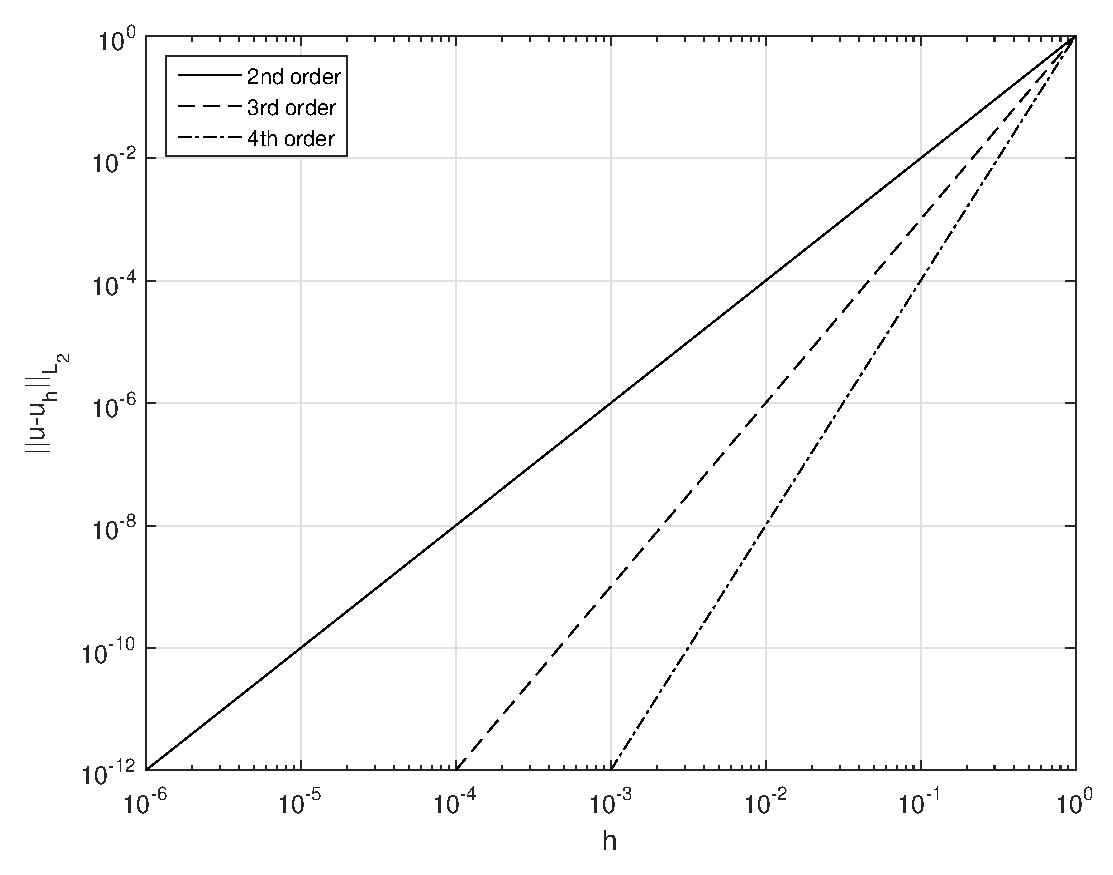
\includegraphics[width=0.485\columnwidth]{images/hconv_larger.eps} \hfill 
{}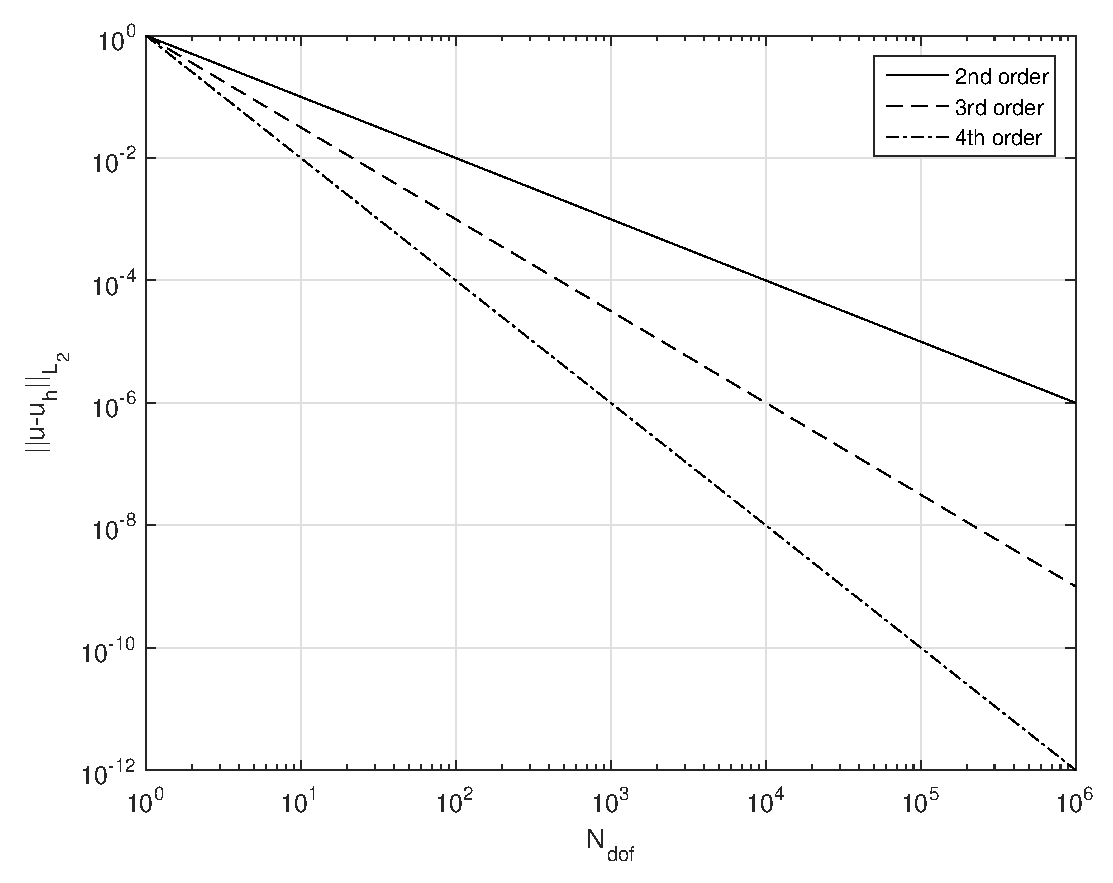
\includegraphics[width=0.485\columnwidth]{images/Nconv_larger.eps}
\end{frame}
%---------------------------
\begin{frame}[t]\frametitle{Polytope Grid Motivation}
         \begin{block}{}{\footnotesize
			\begin{itemize}
				\item <1-> Other physics communities are now employing polytope grids due to decreased cell/face counts (CFD in particular)
				\item <2-> They allow for transition elements between different domain regions
				\item <3-> Hanging nodes from non-conforming meshes are not necessary
				\item <4-> Independently-generated simplicial grids ({\em i.e.} created in parallel) can be stitched together with polytopes without communicating the whole mesh across processors
			\end{itemize}}
         \end{block}
\centering
\only<1>{
\vspace{0.5cm}
{}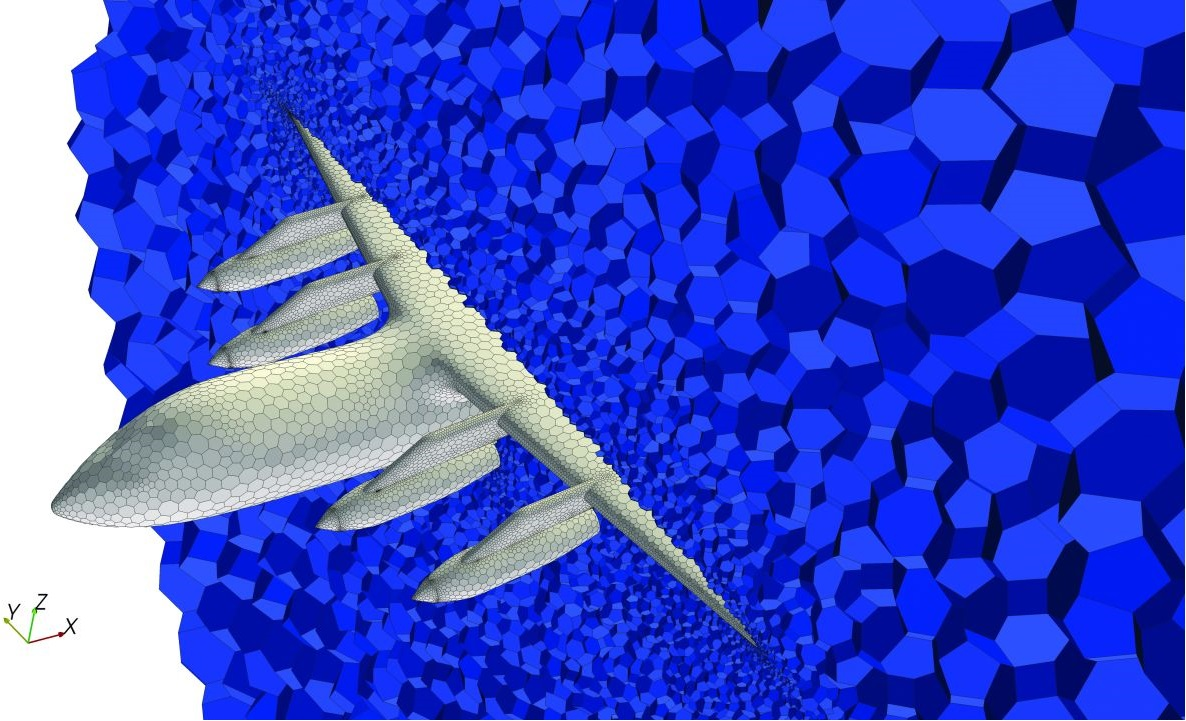
\includegraphics[width=0.45\columnwidth]{images/Polymesh_sized.jpg}
}
\only<2>{
\vspace{0.4cm}
{}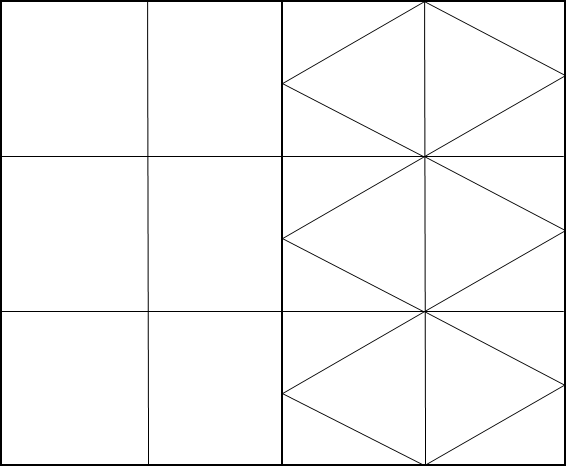
\includegraphics[width=0.4\columnwidth]{images/transition_elements_rev1.png}
}
\only<3>{
\vspace{0.5cm}
{}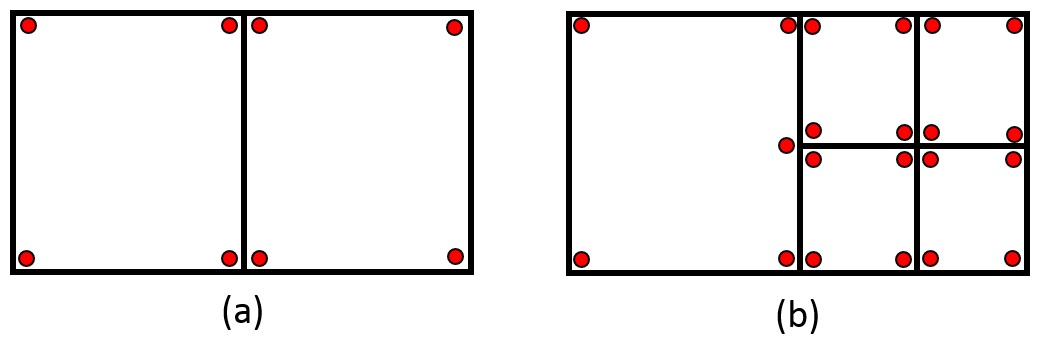
\includegraphics[width=0.55\columnwidth]{images/locally_refined_nodes.png}
}
\only<4>{
\centering
{}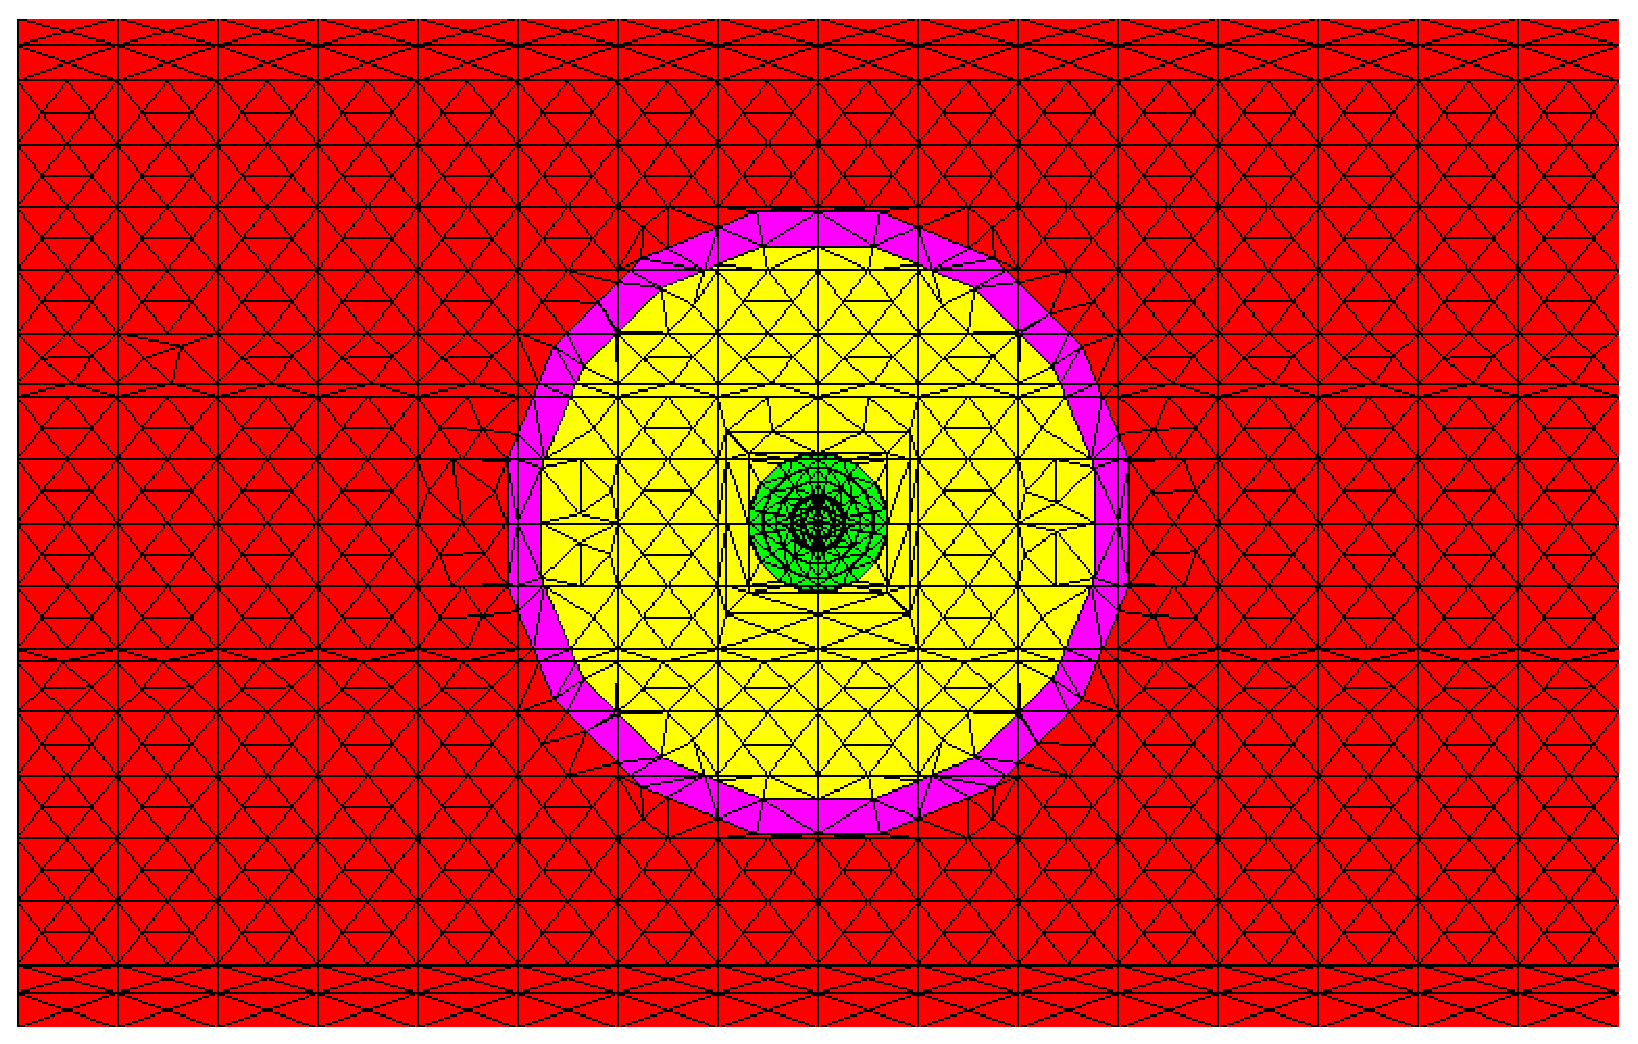
\includegraphics[width=0.52\columnwidth]{images/IM1_30_rot.eps} \hspace{1.0cm}
{}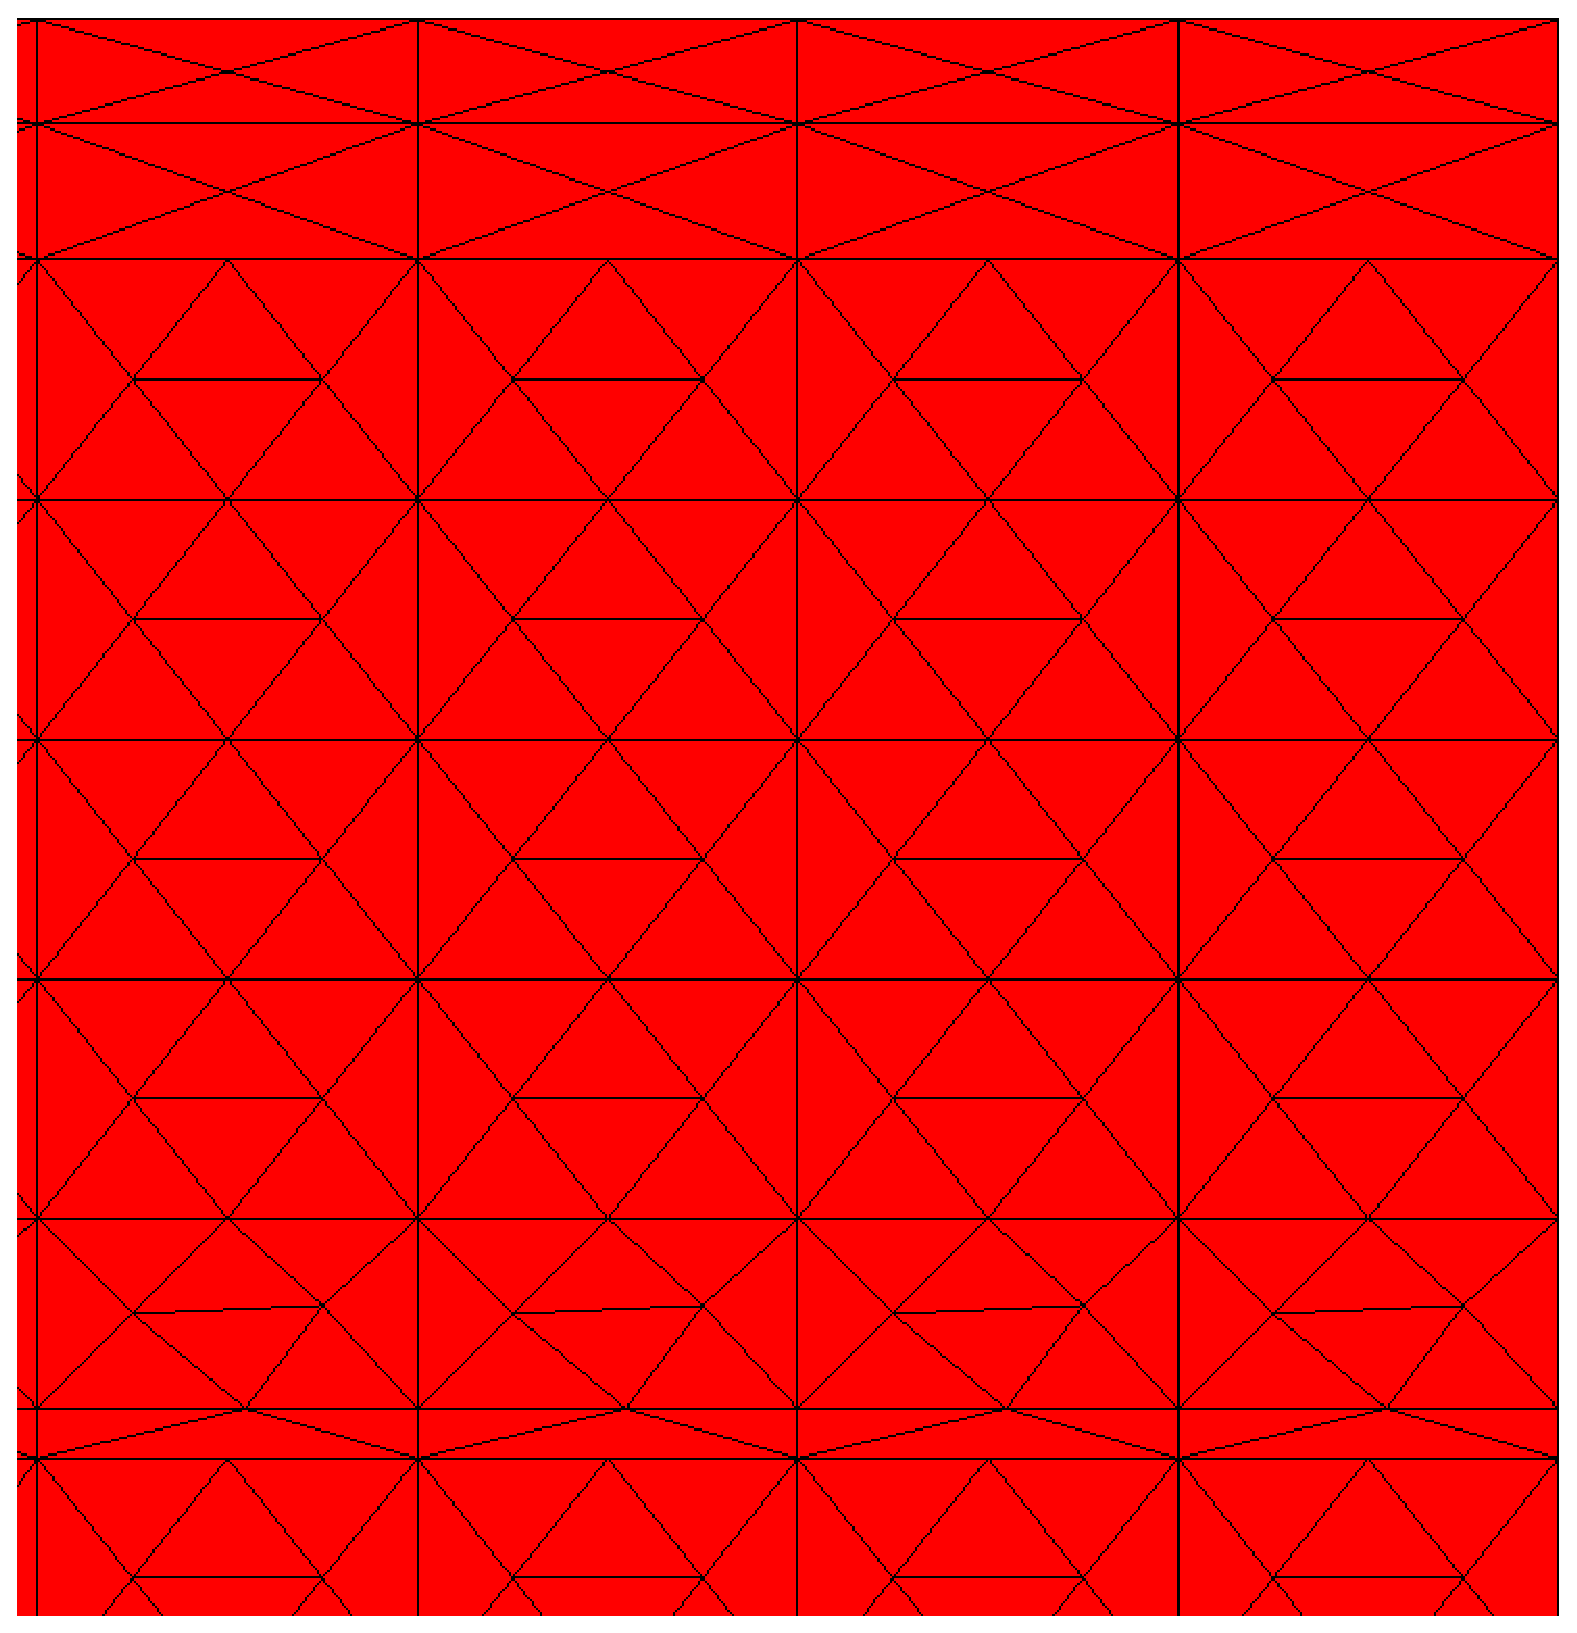
\includegraphics[width=0.345\columnwidth]{images/IM1_zoom.eps}
}
\end{frame}
%---------------------------
%%%%%%%%%%%%%%%%%%%%%%%%%%%%%%%%%%%%%%%%%%%%%%%%%%%%%%%%%%%%%%%%%%%%%%%%%%%%%%%%%%%%%%%%%%%%%%
%
%
\section[POLYFEM]{Polytope Finite Element Basis Functions}
%%%%%%%%%%%%%%%%%%%%%%%%%%%%%%%%%%%%%%%%%%%%%%%%%%
\subsection{}
%---------------------------
\setbeamerfont{frametitle}{size=\normalsize}
\begin{frame}[t]\frametitle{Polytope Finite Elements}
\centering
\begin{block}{2D arbitrary convex/concave polygons}
\centering
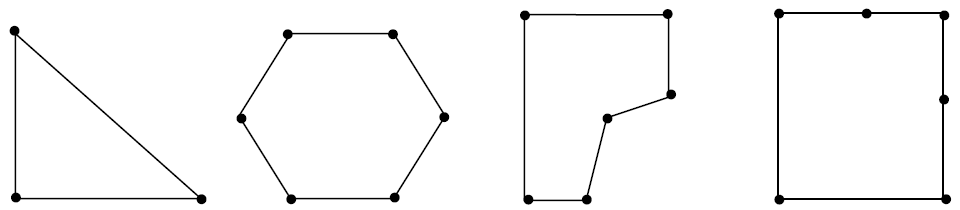
\includegraphics[width=0.70\textwidth]{images/arbitrary_polygons.png}
\end{block}
\vspace{0.5cm}
\begin{block}{3D convex polyhedra}
\centering
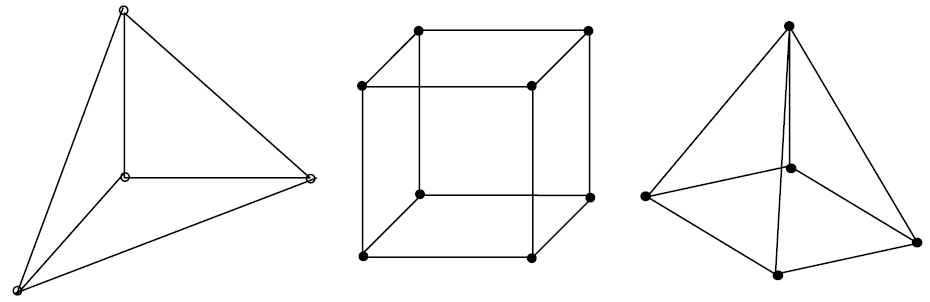
\includegraphics[width=0.70\textwidth]{images/arbitrary_polyhedra.png}
\end{block}
\end{frame}
%---------------------------
\setbeamerfont{frametitle}{size=\normalsize}
\begin{frame}[t]\frametitle{A common class of linear finite elements - the $\mathbb{P}_1$ space}
\begin{columns}
\column{0.48\textwidth} \vspace{-6mm}
\begin{block}{2D $\mathbb{P}_1$ space - reference element} 
\centering
{}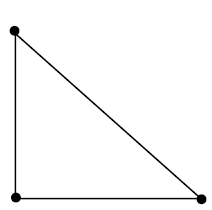
\includegraphics[width=0.55\columnwidth]{images/ref_triangle.png} \vspace{3mm}
\begin{equation*}
\begin{aligned}
\lambda_1 (r,s) &= 1-r-s  \\ 
\lambda_2 (r,s) &= r \\ 
\lambda_3 (r,s) &= s 
\end{aligned}
\end{equation*}
\end{block}
\column{0.48\textwidth}
\begin{block}{3D $\mathbb{P}_1$ space - reference element}
\centering
{}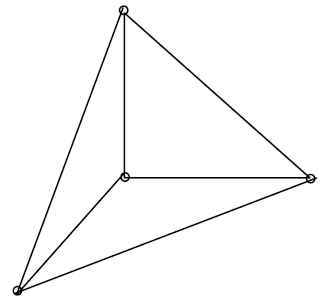
\includegraphics[width=0.60\columnwidth]{images/ref_tet.png} \vspace{3mm}
\begin{equation*}
\begin{aligned}
\lambda_1 (r,s,t) &= 1-r-s - t \\ 
\lambda_2 (r,s,t) &= r \\ 
\lambda_3 (r,s,t) &= s \\
\lambda_4 (r,s,t) &= t \\
\end{aligned}
\end{equation*}
\end{block}
\end{columns}
\end{frame}
%---------------------------
%%%%%%%%%%%%%%%%%%%%%%%%%%%%%%%%%%%%%%%%%%%%%%%%%%%%%%%%%%%%%%%%%%%%%%%%%%%%%%%%%%%%%%%%%%%%%
\subsection{Linear Basis Functions on 2D Polygons}
%%%%%%%%%%%%%%%%%%%%%%%%%%%%%%%%%%%%%%%%%%%%%%%%%%%%%%%%%%%%%%%%%%%%%%%%%%%%%%%%%%%%%%%%%%%%%
\typeout{***********************************************************************************}
\typeout{Linear Basis Functions on 2D Polygons}
%---------------------------
\setbeamerfont{frametitle}{size=\normalsize}
\begin{frame}[t,label=2D_poly]\frametitle{Linear Basis Functions on 2D Polygons}
\centering
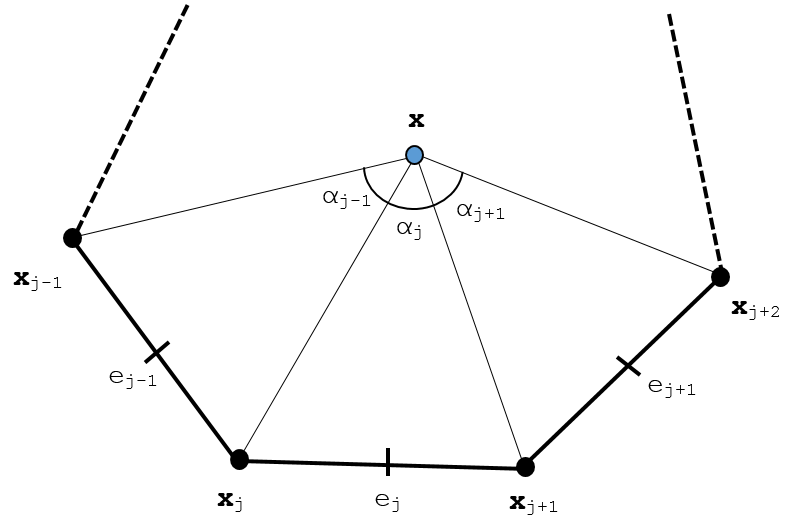
\includegraphics[width=0.40\textwidth]{images/ref_polygon.png}
\vspace{0.75cm}
\only<1>{
\begin{block}{Basis Function Properties - Barycentric Coordinates}
$\lambda_i$ - linear basis function located at vertex $i$ \vspace{0.25cm}
	\begin{enumerate}
	\item $\lambda_i \geq 0$ \vspace{1mm}
	\item $\sum_i \lambda_i = 1$ \vspace{1mm}
	\item $\sum_i \vec{x}_i \lambda_i (\vec{x}) = \vec{x}$ \vspace{1mm}
	\item $\lambda_i (\vec{x}_j) = \delta_{ij}$ 
	\end{enumerate}
\end{block}
}
\only<2>{
\begin{block}{Linear basis functions that we consider}
	\begin{enumerate}
	\item Wachspress rational coordinates*
	\item Piecewise linear (PWL) coordinates*
	\item Mean value coordinates
	\item Maximum entropy coordinates
	\end{enumerate}
\vspace{2mm}
*have been previously analyzed for transport problems
\end{block}
}
\end{frame}
%---------------------------
\setbeamerfont{frametitle}{size=\normalsize}
\begin{frame}[t,label=main_wach]\frametitle{Wachspress Rational Functions (\hyperlink{poly_limits<1>}{\beamergotobutton{Go to extra}})}
\centering
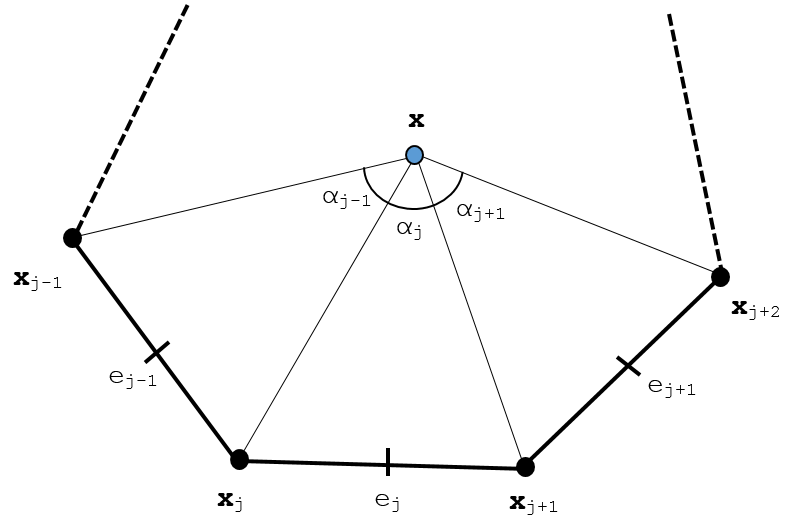
\includegraphics[width=0.40\textwidth]{images/ref_polygon.png}
\vspace{0.3cm}
\begin{block}{}
\begin{equation*}
\lambda_i^W (\vec{x}) = \frac{w_i (\vec{x}) }{ \sum_{j} w_j (\vec{x})}, \qquad w_j (\vec{x}) = \frac{A(\vec{x}_{j-1}, \vec{x}_{j}, \vec{x}_{j+1})}{A(\vec{x}, \vec{x}_{j-1}, \vec{x}_{j}) \, A(\vec{x}, \vec{x}_{j}, \vec{x}_{j+1})}
\end{equation*}
\end{block}
\begin{block}{}
\begin{equation*}
A(\vec{x}_1, \vec{x}_{2}, \vec{x}_{3}) = \frac{1}{2} \left|
\begin{array}{ccc}
1 & 1 & 1 \\
x_1 & x_2 & x_3 \\
y_1 & y_2 & y_3
\end{array} \right|
\end{equation*}
\end{block}
\end{frame}
%---------------------------
\setbeamerfont{frametitle}{size=\normalsize}
\begin{frame}[t]\frametitle{Piecewise Linear (PWL) Functions}
\centering
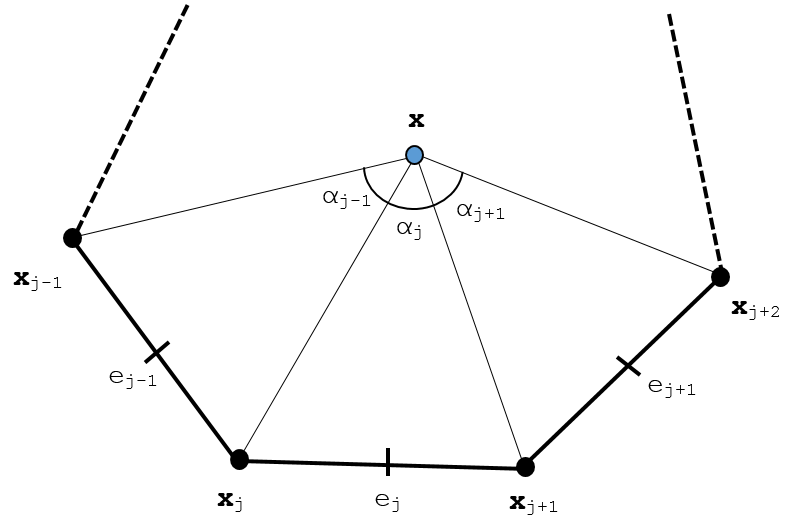
\includegraphics[width=0.40\textwidth]{images/ref_polygon.png}
\vspace{0.3cm}
\begin{block}{}
\begin{equation*}
\lambda_i^{PWL} (\vec{x}) =  t_i (\vec{x}) + \alpha_i t_c (\vec{x})
\end{equation*}
\end{block}
\begin{block}{}
$t_i $ - standard 2D linear function for a triangle $(i,i+1,C)$; 1 at vertex $i$ that linearly decreases to 0 to the cell center and the adjoining vertices \\ \vspace{1mm}
$t_c$ - 2D tent function; 1 at cell center and linearly decreases to 0 to each cell vertex \\ \vspace{1mm}
$\alpha_i = \frac{1}{N_V}$ - weight parameter for vertex $i$ \\ \vspace{1mm}
$N_V$ - number of cell vertices
\end{block}
\end{frame}
%---------------------------
\setbeamerfont{frametitle}{size=\normalsize}
\begin{frame}[t,label=main_mv]\frametitle{Mean Value Coordinates (\hyperlink{poly_limits<1>}{\beamergotobutton{Go to extra}})}
\centering
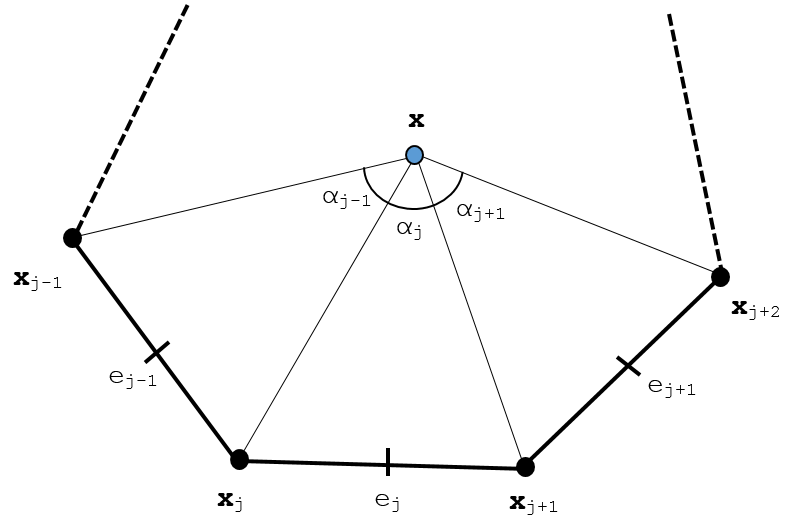
\includegraphics[width=0.40\textwidth]{images/ref_polygon.png}
\vspace{0.3cm}
\only<1>{
\begin{block}{Preserve piecewise linear harmonic maps over triangulations}
\begin{equation*}
\frac{\partial^2 u}{\partial x^2} + \frac{\partial^2 u}{\partial y^2} = 0, \qquad u(\vec{r}) = u_0 , \, \vec{r} \in \partial \mathcal{D} 
\end{equation*} \\
\vspace{1.0cm}
$u(\vec{r})$ - piecewise linear function on the cell boundary
\end{block}
}
\only<2>{
\begin{block}{}
\begin{equation*}
\lambda_i^{MV} (\vec{x}) = \frac{w_i (\vec{x}) }{ \sum_{j} w_j (\vec{x})}, \qquad w_j (\vec{x}) = \frac{\tan(\alpha_{j-1} / 2) + \tan(\alpha_j / 2)}{|\vec{x}_j - \vec{x}|}
\end{equation*}
\end{block}
\begin{block}{Limit as $\vec{x} \rightarrow \vec{x}_j$}
\vspace{-0.25cm}
\begin{columns}
\column{0.5\textwidth}
\centering
\begin{equation*}
\lim_{\vec{x} \rightarrow \vec{x}_j} \tan(\alpha_{j-1} / 2) + \tan(\alpha_j / 2) = 0
\end{equation*}
\column{0.1\textwidth}
\centering
$\longrightarrow$
\column{0.4\textwidth}
\centering
\begin{equation*}
\lim_{\vec{x} \rightarrow \vec{x}_j}  w_j (\vec{x}) = 1
\end{equation*}
\end{columns}
\end{block}
}
\end{frame}
%---------------------------
\setbeamerfont{frametitle}{size=\normalsize}
\begin{frame}[t,label=main_me]\frametitle{Maximum Entropy Coordinates (\hyperlink{poly_limits<1>}{\beamergotobutton{Go to extra}})}
\centering
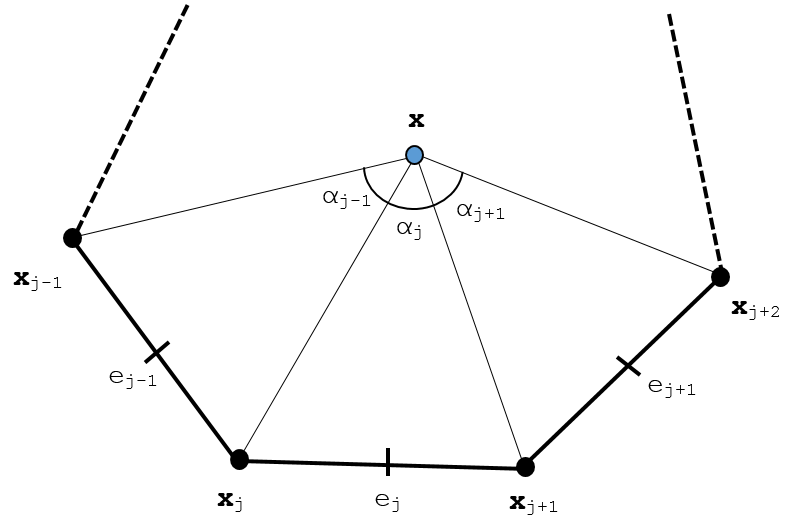
\includegraphics[width=0.40\textwidth]{images/ref_polygon.png}
\vspace{0.3cm}
\only<1>{
\begin{block}{Constrained optimization problem - Shannon Entropy}
\begin{equation*}
\max\displaylimits_{\lambda(\vec{x})}  H(\lambda, m), \qquad  H(\lambda, m) = - \sum\displaylimits_{i} \lambda_i (\vec{x}) \ln \left(   \frac{\lambda_i(\vec{x})}{m_i(\vec{x})} \right)
\end{equation*} \\ \vspace{3mm}
\begin{equation*}
\sum\displaylimits_{i} \lambda_i (\vec{x}) = 1, \qquad \sum\displaylimits_{i} \lambda_i (\vec{x}) ( \vec{x}_i - \vec{x} ) = \vec{0}
\end{equation*}
\end{block}
}
\only<2>{
\begin{block}{}
\begin{equation*}
\lambda_i^{ME} (\vec{x}) = \frac{w_i (\vec{x}) }{ \sum_{j} w_j (\vec{x})}, \qquad w_j (\vec{x}) = m_j(\vec{x}) \exp(- \omega^* \cdot (\vec{x}_j - \vec{x}))
\end{equation*}
\end{block}
\begin{block}{}{\small
\begin{equation*}
\mathcal{L} (\lambda, \omega_0, \omega) = - \sum\displaylimits_{i} \lambda_i (\vec{x}) \ln \left(   \frac{\lambda_i(\vec{x})}{m_i(\vec{x})} \right) - \omega_0 \left(  \sum\displaylimits_{i}  \lambda_i (\vec{x}) -1  \right) - \omega \cdot  \left(  \sum\displaylimits_{i}  \lambda_i (\vec{x}) (\vec{x}_i - \vec{x})  \right)
\end{equation*}}
\end{block}
}
\only<3>{
\begin{block}{}
\begin{equation*}
\lambda_i^{ME} (\vec{x}) = \frac{w_i (\vec{x}) }{ \sum_{j} w_j (\vec{x})}, \qquad w_j (\vec{x}) = m_j(\vec{x}) \exp(- \omega^* \cdot (\vec{x}_j - \vec{x}))
\end{equation*}
\end{block}
\begin{block}{}
\begin{equation*}
\omega^* = \text{argmin} \, F(\omega, \vec{x})  \qquad F(\omega, \vec{x}) = \ln \left(  \sum_j w_j (\vec{x})  \right)
\end{equation*}
\end{block}
}
\end{frame}
%---------------------------
\begin{frame}[t]\frametitle{Finite element architecture}
\begin{block}{Mass Matrix - element $K$}
\begin{equation*}
{\bf M}^K = \int_{K} d\vec{r} \, \lambda (\vec{x}) \, \lambda^T (\vec{x})  =  \sum\displaylimits_{q=1}^{N_q^K} w_q^K \, \lambda (\vec{x}_q^K) \, \lambda^T (\vec{x}_q^K) 
\end{equation*}
\end{block}
\begin{block}{Advection Matrix - element $K$}
\begin{equation*}
{\bf G}^K = \int_{K} d\vec{r} \, \vec{\nabla} \lambda (\vec{x}) \, \lambda^T (\vec{x}) = \sum\displaylimits_{q=1}^{N_q^K}  w_q^K \, \vec{\nabla} \lambda (\vec{x}_q^K) \, \lambda^T (\vec{x}_q^K) 
\end{equation*}
\end{block}
\begin{block}{Surface Matrix - face $f$ for element $K$}
\begin{equation*}
{\bf N}_f^K = \int_{f} ds \, \lambda (\vec{x}) \, \lambda^T (\vec{x})  = \sum\displaylimits_{q=1}^{N_f}  w_q^f \, \lambda (\vec{x}_q^f) \, \lambda^T (\vec{x}_q^f) 
\end{equation*}
\end{block}
\end{frame}
%---------------------------
\setbeamerfont{frametitle}{size=\normalsize}
\begin{frame}[t]\frametitle{Summary of the 2D Linear Basis Functions}
\centering
\vspace{1cm}
\begin{table}
\footnotesize
\begin{tabular}{|c|c|c|c|c|}
\hline
Basis Function & Dimension & Polytope Types & Integration & Direct/Iterative \\
\hline \hline
Wachspress	&2D/3D&	Convex*&	Numerical	&Direct\\ \hline
PWL&	1D/2D/3D&	Convex/Concave&	Analytical	&Direct\\ \hline
Mean Value&	2D**&	Convex/Concave&	Numerical	&Direct\\ \hline
Max Entropy&	1D/2D/3D	&Convex/Concave&	Numerical&	Iterative***\\ \hline
\end{tabular}
\end{table}
\vspace{0.5cm}
\begin{block}{}
* - weak convexity for Wachspress coordinates does not cause blow up\\
** - mean value 3D analogue only applicable triangular-faceted polyhedra \\
*** - maximum entropy minimization solved via Newton's Method 
\end{block}
\end{frame}
%---------------------------
%%%%%%%%%%%%%%%%%%%%%%%%%%%%%%%%%%%%%%%%%%%%%%%%%%
\subsection{Quadratic Serendipity Basis Functions on 2D Polygons}
%%%%%%%%%%%%%%%%%%%%%%%%%%%%%%%%%%%%%%%%%%%%%%%%%%%%%%%%%%%%%%%%%%%%%%%%%%%%%%%%%%%%%%%%%%%%%
\typeout{***********************************************************************************}
%---------------------------
\begin{frame}[t]\frametitle{Quadratic Serendipity Basis Functions on 2D Polygons}
\begin{block}{}
\begin{enumerate}
	\item <1-> Form the linear barycentric functions - \{$\lambda_i$\}
	\item <2-> Construct the pairwise products -  \{$\mu_{ab}$\}
	\item <3-> Eliminate the interior nodes to form a serendipity basis - \{$\xi_{ij}$\}
\end{enumerate}
\end{block}
\vspace{1cm}
\begin{columns}[c]
\column{0.28\textwidth}
\centering
\only<1-3>{
{}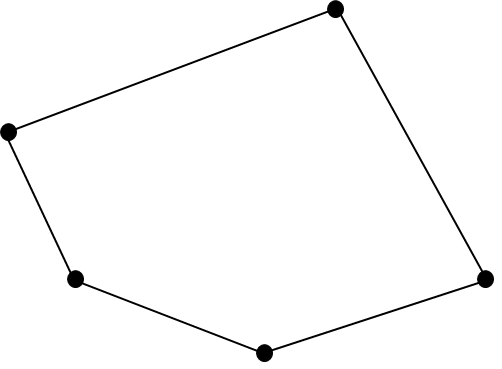
\includegraphics[width=0.9\columnwidth]{images/rand_linear.png} \\
\{$\lambda_i$\} \\
Linear
}
\column{0.08\textwidth}
\only<2-3>{
$\longrightarrow$
}
\column{0.28\textwidth}
\centering
\only<2-3>{
{}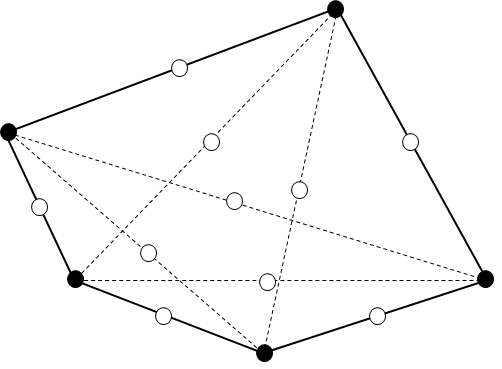
\includegraphics[width=0.9\columnwidth]{images/rand_quadratic.png} \\
\{$\mu_{ab}$\} \\
Quadratic
}
\column{0.08\textwidth}
\only<3>{
$\longrightarrow$
}
\column{0.28\textwidth}
\centering
\only<3>{
{}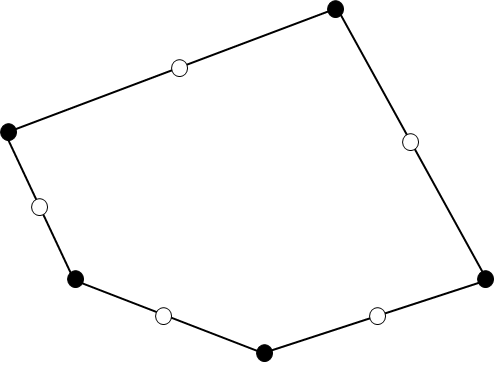
\includegraphics[width=0.9\columnwidth]{images/rand_serendipity.png} \\
\{$\xi_{ij}$\} \\
Serendipity
}
\end{columns}
\end{frame}
%---------------------------
\begin{frame}[t]\frametitle{Pairwise products of the barycentric basis functions - $\mu_{ab} = \lambda_a \lambda_b$}
\only<1>{
\centering
{}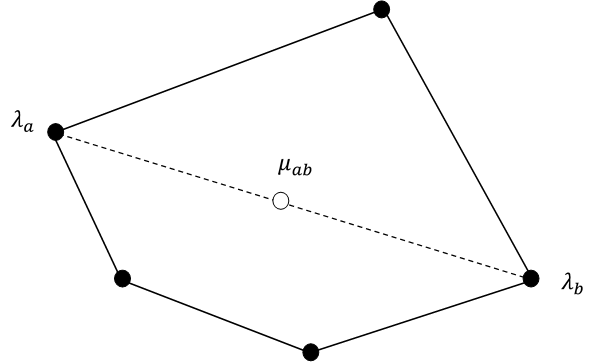
\includegraphics[width=0.75\columnwidth]{images/rand_quad_ab.png} 
}
\only<2>{
\begin{block}{Necessary Precision Properties}
\begin{columns}
\column{0.62\textwidth}
\begin{equation*}
\sum_{aa \in V} \mu_{aa} + \sum_{ab \in E \cup D} 2 \mu_{ab} = 1
\end{equation*}
\begin{equation*}
\sum_{aa \in V} \vec{x}_{aa} \mu_{aa} + \sum_{ab \in E \cup D} 2 \vec{x}_{ab} \mu_{ab} = \vec{x}
\end{equation*}
\begin{equation*}
\sum_{aa \in V} \vec{x}_{a} \vec{x}_{a}^T \mu_{aa} + \sum_{ab \in E \cup D} \left(  \vec{x}_{a} \vec{x}_{b}^T + \vec{x}_{b} \vec{x}_{a}^T  \right) \mu_{ab} = \vec{x} \vec{x}^{T}
\end{equation*}
\column{0.03\textwidth}
\column{0.35\textwidth}
{\small
$V$ - vertex nodes \\
$E$ - face midpoint nodes \\
$D$ - interior diagonal nodes
}
\end{columns}
\end{block}
\begin{block}{Further Notation/Notes}
\begin{equation*}
\vec{x}_{ab} = \frac{\vec{x}_{a} + \vec{x}_{b}}{2}, \qquad \mu_{ab} = \lambda_a \lambda_b
\end{equation*}
\vspace{0.4cm}
\begin{equation*}
\mu^{K}_{ab}(\vec{r}) = 0, \qquad \left\{ ab \in D , \, \vec{r} \in \partial K  \right\}
\end{equation*}
\end{block}
}
\end{frame}
%---------------------------
\begin{frame}[t]\frametitle{Eliminate interior nodes to form serendipity basis}
\only<1>{
\centering
{}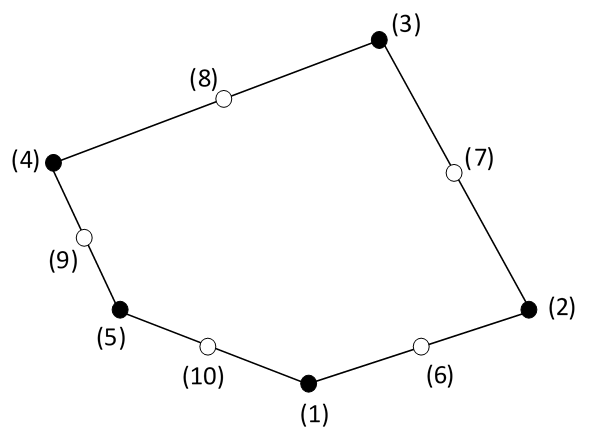
\includegraphics[width=0.75\columnwidth]{images/rand_ser_numbering.png} 
}
\only<2>{
\begin{block}{Serendipity Precision Properties}{\small
\begin{columns}
\column{0.50\textwidth}
\begin{equation*}
\sum_{ii \in V} \xi_{ii} + \sum_{i(i+1) \in E} 2 \xi_{i(i+1)} = 1
\end{equation*}
\begin{equation*}
\sum_{ii \in V} \vec{x}_{ii} \xi_{ii} + \sum_{i(i+1) \in E} 2 \vec{x}_{i(i+1)} \xi_{i(i+1)} = \vec{x}
\end{equation*}
\begin{equation*}
\sum_{ii \in V} \vec{x}_{i} \vec{x}_{i}^T \xi_{ii} + \sum_{i(i+1) \in E} \left(  \vec{x}_{i} \vec{x}_{i+1}^T + \vec{x}_{i+1} \vec{x}_{i}^T  \right) \xi_{i(i+1)} = \vec{x} \vec{x}^{T}
\end{equation*}
\column{0.03\textwidth}
\column{0.35\textwidth}
$\xi_{ii}$ - basis function at vertex $i$\\ \vspace{1mm}
$\xi_{i(i+1)}$ - basis function at face midpoint between vertices ($i, i+1$)
\end{columns}
}\end{block}
\begin{block}{Reduction Problem - $\left[ \xi \right] := \mathbb{A}  \left[ \mu \right]$}{\small
\begin{equation*}
\mathbb{A} = 
\left[
\begin{array}{ccccc}
c_{11}^{11} & \ldots & c_{ab}^{11} & \ldots & c_{(n-2)n}^{11} \\
\ldots&\ddots&\vdots&\ddots&\vdots \\
c_{11}^{ij} & \ldots & c_{ab}^{ij} & \ldots & c_{(n-2)n}^{ij} \\
\ldots&\ddots&\vdots&\ddots&\vdots \\
c_{11}^{n(n+1)} & \ldots & c_{ab}^{n(n+1)} & \ldots & c_{(n-2)n}^{n(n+1)} 
\end{array}
\right]
\end{equation*}
}\end{block}
}
\only<3>{
\vspace{-3mm}
\begin{block}{Constant Precision}{\footnotesize
\begin{equation*}
\begin{aligned}
\sum\displaylimits_{ii \in V} c_{aa}^{ii} + \sum\displaylimits_{i(i+1) \in E} 2 c_{aa}^{i(i+1)} &= 1 , \qquad \forall aa \in V \\
\sum\displaylimits_{ii \in V} c_{ab}^{ii} + \sum\displaylimits_{i(i+1) \in E} 2 c_{ab}^{i(i+1)} &= 2 , \qquad \forall ab \in E \cup D
\end{aligned}
\end{equation*}
}\end{block}
\begin{block}{Linear Precision}{\footnotesize
\begin{equation*}
\begin{aligned}
\sum\displaylimits_{ii \in V} c_{aa}^{ii} \vec{x}_{ii} + \sum\displaylimits_{i(i+1) \in E} 2 c_{aa}^{i(i+1)} \vec{x}_{i (i+1)} &= \vec{x}_{aa} , \qquad \forall aa \in V \\
\sum\displaylimits_{ii \in V} c_{ab}^{ii} \vec{x}_{ii} + \sum\displaylimits_{i(i+1) \in E} 2 c_{ab}^{i(i+1)} \vec{x}_{i (i+1)} &= 2 \vec{x}_{ab} , \qquad \forall ab \in E \cup D
\end{aligned}
\end{equation*}
}\end{block}
\begin{block}{Quadratic Precision}{\footnotesize
\begin{equation*}
\begin{aligned}
\sum\displaylimits_{ii \in V} c_{aa}^{ii} \vec{x}_{i} \vec{x}_{i}^T + \sum\displaylimits_{i(i+1) \in E} 2 c_{aa}^{i(i+1)} \left(  \vec{x}_{i} \vec{x}_{i+1}^T + \vec{x}_{i+1} \vec{x}_{i}^T  \right) &= \vec{x}_{a} \vec{x}_{a}^T , \qquad &\forall aa \in V \\
\sum\displaylimits_{ii \in V} c_{ab}^{ii} \vec{x}_{i} \vec{x}_{i}^T + \sum\displaylimits_{i(i+1) \in E} 2 c_{ab}^{i(i+1)} \left(  \vec{x}_{i} \vec{x}_{i+1}^T + \vec{x}_{i+1} \vec{x}_{i}^T  \right) &= \vec{x}_{a} \vec{x}_{b}^T + \vec{x}_{b} \vec{x}_{a}^T, \qquad &\forall ab \in E \cup D
\end{aligned}
\end{equation*}
}\end{block}
}
\end{frame}
%---------------------------
\begin{frame}[t]{Special case - bilinear coordinates on the unit square}
\vspace{-0.2cm}
\begin{block}{Bilinear coordinates and quadratic extension}{\footnotesize
\vspace{-0.15cm}
\begin{columns}
\column{0.3\textwidth}
\begin{equation*}
\begin{aligned}
\lambda_1 &= (1-x)(1-y)  \\
\lambda_2 &= x(1-y) \\
\lambda_3 &= xy  \\
\lambda_4 &= (1-x)y
\end{aligned}
\end{equation*}
\column{0.1\textwidth}
\column{0.6\textwidth}
\begin{equation*}
\begin{aligned}
\mu_{11} &= (1-x)^2 (1-y)^2&   &\mu_{12} = (1-x)x(1-y)^2 \\
\mu_{22} &= x^2 (1-y)^2&  &\mu_{23} = x^2y(1-y) \\
\mu_{33} &= x^2 y^2&  &\mu_{34} = (1-x)xy^2 \\
\mu_{44} &= (1-x)^2 y^2&  &\mu_{41} = (1-x)^2y(1-y) \\
\mu_{13} &= (1-x)x (1-y)y& &\mu_{24} = (1-x)x (1-y)y
\end{aligned}
\end{equation*}
\end{columns}
}\end{block}
\vspace{-0.3cm}
\begin{columns}
\column{0.58\textwidth}
\centering
\begin{block}{Reduction matrix}{\scriptsize
\begin{equation*}
\mathbb{A} = 
\left[
\begin{array}{cccccccccc}
1&0&0&0&0&0&0&0&-1&0 \\
0&1&0&0&0&0&0&0&0&-1\\
0&0&1&0&0&0&0&0&-1&0 \\
0&0&0&1&0&0&0&0&0&-1 \\
0&0&0&0&1&0&0&0&1/2&1/2 \\
0&0&0&0&0&1&0&0&1/2&1/2 \\
0&0&0&0&0&0&1&0&1/2&1/2 \\
0&0&0&0&0&0&0&1&1/2&1/2 
\end{array}
\right]
\end{equation*}
}\end{block}
\column{0.38\textwidth}
\centering
\begin{block}{Serendipity coordinates}{\scriptsize
\begin{equation*}
\begin{aligned}
\xi_{11} &= (1-x) (1-y)(1-x-y) \\
\xi_{22} &= x(1-y)(x-y)\\
\xi_{33} &= x y(-1+x+y) \\
\xi_{44} &= (1-x) y(y-x) \\
\xi_{12} &= (1-x)x(1-y) \\
\xi_{23} &= xy(1-y) \\
\xi_{34} &= (1-x)xy \\
\xi_{41} &= (1-x)y(1-y) 
\end{aligned}
\end{equation*}
}\end{block}
\end{columns}
\end{frame}
%---------------------------
%%%%%%%%%%%%%%%%%%%%%%%%%%%%%%%%%%%%%%%%%%%%%%%%%%
\subsection{Linear Basis Functions on 3D Polyhedra}
%%%%%%%%%%%%%%%%%%%%%%%%%%%%%%%%%%%%%%%%%%%%%%%%%%%%%%%%%%%%%%%%%%%%%%%%%%%%%%%%%%%%%%%%%%%%%
\typeout{***********************************************************************************}
\typeout{Polytope Finite Element Basis Functions}
%---------------------------
\setbeamerfont{frametitle}{size=\large}
\begin{frame}[t]{Linear Basis Functions on 3D Polyhedra}
\begin{block}{Linear basis functions and convex polyhedra only for 3D}{\small
\begin{itemize}
\item The 2D quadratic serendipity formulation is more arduous in 3D
\item Intercell coupling is not straightforward for concave polyhedra
\item Focus on 3D PWL functions
\item Focus on 3D parallelepipeds and extruded convex polygons (convex prisms)
\end{itemize}}
\end{block}
\begin{block}{3D PWL basis functions}{\small
\begin{equation*}
b_i (\vec{x})  = t_i  (\vec{x})  + \sum_{f=1}^{F_i} \beta_f^i  t_f (\vec{x}) + \alpha_i t_c  (\vec{x}) 
\end{equation*}
}\end{block}
\begin{block}{}{\footnotesize
$t_i$ - standard 3D linear function for a tet $(i,i+1,f_c,K_c)$; 1 at vertex $i$, linearly decreases to 0 to the cell center, each adjoining face center, and each adjoining vertex\\ \vspace{0.5mm}
$t_c$ - 3D tent function; 1 at cell center, linearly decreases to 0 at all vertices and face centers \\ \vspace{0.5mm}
$t_f$ - face tent function; 1 at face center, linearly decreases to 0 at each face vertex and cell center\\ \vspace{0.5mm}
$\alpha_i = \frac{1}{N_V}$ - weight parameter for vertex $i$\\ \vspace{0.5mm}
$\beta_f^i = \frac{1}{N_f}$ - weight parameter for face $f$ touching vertex $i$
}\end{block}
\end{frame}
%---------------------------
%%%%%%%%%%%%%%%%%%%%%%%%%%%%%%%%%%%%%%%%%%%%%%%%%%%%%%%%%%%%%%%%%%%%%%%%%%%%%%%%%%%%%%%%%%%%%%
%
%
\section[DSA on Polytopes]{Diffusion Synthetic Acceleration on Polytopes}
\subsection{Theory}
%%%%%%%%%%%%%%%%%%%%%%%%%%%%%%%%%%%%%%%%%%%%%%%%%%%%%%%%%%%%%%%%%%%%%%%%%%%%%%%%%%%%%%%%%%%%%
\typeout{***********************************************************************************}
\typeout{DSA}
%---------------------------
\begin{frame}[t]\frametitle{Diffusion Synthetic Acceleration}
\begin{block}{Transport iteration and error}{\small
\begin{columns}
\column{0.48\textwidth}
\begin{equation*}
\begin{aligned}
&{\bf L} \psi = {\bf B} \phi + {\bf C} \phi + {\bf Q} \\
&{\bf L} \psi^{(\ell+1/2)} = {\bf B} \phi^{(\ell+1/2)} + {\bf C} \phi^{(\ell)} + {\bf Q} \\
&\noindent\rule{5.5cm}{0.4pt} \\
&{\bf L} \delta \psi^{(\ell+1/2)} - {\bf B}' \delta \phi^{(\ell+1/2)} = {\bf R}^{(\ell+1/2)}
\end{aligned}
\end{equation*}
\column{0.48\textwidth}
\begin{equation*}
\begin{aligned}
\delta \psi^{(\ell+1/2)} &\equiv \psi - \psi^{(\ell+1/2)} \\
\delta \phi^{(\ell+1/2)} &\equiv {\bf D} \delta \psi^{(\ell+1/2)}
\end{aligned}
\end{equation*}
\end{columns}}
\end{block}
\begin{block}{Error approximation and update}{\small
If we could exactly solve for the error, then the solution could be obtained immediately:
\begin{equation*}
\phi^{(\ell+1)} = \phi^{(\ell+1/2)} + \delta \phi^{(\ell+1/2)}
\end{equation*}
However, this is just as difficult as the full transport problem. Instead, we estimate the error using low-order operators:
\begin{equation*}
\tilde{{\bf L}} \delta \psi^{(\ell+1/2)} - \tilde{{\bf B}}' \delta \phi^{(\ell+1/2)} = \tilde{{\bf R}}^{(\ell+1/2)}
\end{equation*}
}\end{block}
\end{frame}
%---------------------------
\begin{frame}[t]\frametitle{Various DSA Implementations}
\begin{block}{Historical DSA Work}
\begin{itemize}
	\item Gelbard and Hageman (G\&B) - efficient convergence on fine meshes
	\item Reed - showed that G\&B diverged for coarse meshes
	\item Alcouffe - consistency yields efficiency and robustness
\end{itemize}
\end{block}
\begin{block}{Fully-consistent DSA schemes}
\begin{itemize}
	\item Larsen fully-consistent four step
	\item Fully-consist DSA (FCDSA)
\end{itemize}
\end{block}
\begin{block}{Partially-consistent DSA schemes}
\begin{itemize}
	\item Modified four step (M4S)
	\item Waering-Larsen-Adams (WLA)
	\item Modified Interior Penalty DSA (MIP)
\end{itemize}
\end{block}
\end{frame}
%---------------------------
\subsection{MIP Diffusion Form}
%%%%%%%%%%%%%%%%%%%%%%%%%%%%%%%%%%%%%%%%%%%%%%%%%%%%%%%%%%%%%%%%%%%%%%%%%%%%%%%%%%%%%%%%%%%%%
\typeout{***********************************************************************************}
\typeout{DSA}
%---------------------------
\setbeamerfont{frametitle}{size=\small}
\begin{frame}[t]\frametitle{The diffusion equation is used as our low-order operator}
	\begin{block}{The Diffusion Equation}\vspace{-0.25cm} {\small 
     		\begin{align*}
 	 		{ \small -{\bf \nabla} \cdot D {\bf \nabla} \Phi ({\bf r}) + \sigma \Phi ({\bf r}) = q ({\bf r}), \qquad  {\bf r} \in \mathcal{D} }
        	\end{align*} }\vspace{-0.25cm}
        	\end{block}
        	\begin{block}{General Boundary Conditions} \vspace{-0.4cm} {\small 
		\begin{align*}
 	 		{ \small \Phi ({\bf r})  = \Phi_0 ({\bf r}) , \qquad {\bf r} \in \partial \mathcal{D}^d } \\
 	 		{ \small -D \partial_n \Phi ({\bf r})  = J_0 ({\bf r}) , \qquad {\bf r} \in \partial \mathcal{D}^n } \\
 	 		{ \small \frac{1}{4} \Phi ({\bf r})  + \frac{1}{2}D \partial_n \Phi ({\bf r})  = J^{inc} ({\bf r}) ,  \qquad {\bf r} \in \partial \mathcal{D}^r}
        		\end{align*} } \vspace{-0.25cm}
    \end{block}
	\begin{block}{Desirable diffusion form properties} {\small 
	\begin{itemize}
		\item Can handle concave and degenerate polytope cells
		\item Symmetric Positive-Definite (SPD) 
		\item Availability of suitable preconditioners
		\item Agnostic of directionality of interior faces
	\end{itemize} }
	\end{block}
\end{frame}
%---------------------------
\begin{frame}[t]\frametitle{Symmetric Interior Penalty (SIP) Form}
	\begin{block}{Bilinear Form}{\small
		\begin{gather*}
			 a( \Phi, b)  = \Big<  D \vec{\nabla}  \Phi , \vec{\nabla} b  \Big>_{\mathcal{D}} + \Big<  \sigma   \Phi ,  b  \Big>_{\mathcal{D}}    \\
			+  \Big\{ \kappa_e^{SIP} [\![   \Phi ]\!] , [\![  b ]\!]\Big\}_{E_h^i} - \Big\{  [\![   \Phi ]\!] , \{\!\{  D \partial_n b \}\!\}\Big\}_{E_h^i} -\Big\{ \{\!\{  D \partial_n  \Phi \}\!\} , [\![ b ]\!]\Big\}_{E_h^i} \\
			+ \Big\{ \kappa_e^{SIP}   \Phi ,   b \Big\}_{\partial \mathcal{D}^d} - \Big\{   \Phi  ,  D \partial_n b \Big\}_{\partial \mathcal{D}^d} - \Big\{   D 				\partial_n  \Phi ,   b \Big\}_{\partial \mathcal{D}^d}  +  \frac{1}{2} \Big\{    \Phi ,   b \Big\}_{\partial \mathcal{D}^r}
        	\end{gather*} }
\end{block}
\begin{block}{Linear Form}{\small
		\begin{align*}
			\ell (b) = \Big<  q, b  \Big>_{\mathcal{D}}  - \Big\{   J_{0}, b  \Big\}_{\partial \mathcal{D}^n} +  2 \Big\{   J_{inc}, b  \Big\}_{\partial 				\mathcal{D}^r} \\ + \Big\{ \kappa_e^{SIP}   \Phi_0 ,   b \Big\}_{\partial \mathcal{D}^d} - \Big\{   \Phi_0  ,  D \partial_n b \Big\}_{\partial 					\mathcal{D}^d} 
        	\end{align*} }
    \end{block}
\end{frame}
%---------------------------
\begin{frame}[t]\frametitle{SIP Penalty Coefficient}
\begin{block}{}{
	\begin{equation*}
		\kappa_e^{SIP} \equiv 
		\begin{cases}
		\frac{C_B}{2} \left(  \frac{D^+}{h^+} + \frac{D^-}{h^-}  \right) & , e \in E_h^i \\
		C_B \frac{D^-}{h^-}  & , e \in \partial \mathcal{D}
		\end{cases}
	\end{equation*}}
	\begin{equation*}
		C_B = c p (p+1)
	\end{equation*}
\end{block}
\begin{block}{}
$c$ - user defined constant ($c \geq 1$) \\
$p$ - polynomial order of the finite element basis ($1,2,3,...$) \\
$D^{(+/-)}$ - diffusion coefficient defined on the positive/negative side of a face\\
$h^{(+/-)}$ - orthogonal projection defined on the positive/negative side of a face
\end{block}
\begin{block}{}
	\begin{equation*}
		u^{\pm} = \lim_{s \rightarrow 0^{\pm}} u ({\bf r} + s {\bf n})
	\end{equation*}
\end{block}
\end{frame}
%---------------------------
\begin{frame}[t]\frametitle{Modified Interior Penalty (MIP) Form}
	\begin{block}{Diffusion Form}{\footnotesize
		\begin{gather*}
			 \Big<  D \vec{\nabla} \delta \Phi , \vec{\nabla} b  \Big>_{\mathcal{D}} + \Big<  \sigma \delta  \Phi ,  b  \Big>_{\mathcal{D}}    \\
			+  \Big\{ \kappa_e^{MIP} [\![ \delta  \Phi ]\!] , [\![  b ]\!]\Big\}_{E_h^i} - \Big\{  [\![  \delta \Phi ]\!] , \{\!\{  D \partial_n b \}\!\}\Big\}_{E_h^i} -\Big\{ \{\!\{  D \partial_n \delta \Phi \}\!\} , [\![ b ]\!]\Big\}_{E_h^i} \\
			+ \Big\{ \kappa_e^{MIP} \delta  \Phi ,   b \Big\}_{\partial \mathcal{D}^{vac}} -  \frac{1}{2} \Big\{  \delta \Phi  ,  D \partial_n b \Big\}_{\partial \mathcal{D}^{vac}} -  \frac{1}{2} \Big\{   D \partial_n \delta \Phi ,   b \Big\}_{\partial \mathcal{D}^{vac}}  \\
 = \Big<  R , b  \Big>_{\mathcal{D}}  +  \Big\{  \delta J_{inc}, b  \Big\}_{\partial \mathcal{D}^{ref}}
        	\end{gather*} }
\end{block}
	\begin{block}{MIP Penalty Term}{\footnotesize
		\begin{align*}
			\kappa_e^{MIP} = \max(\frac{1}{4},  \kappa_e^{SIP})
		\end{align*} }
	\end{block}
\end{frame}
%---------------------------
\begin{frame}[t]\frametitle{Two-Grid Acceleration - Ideal for graphite and heavy-water configurations}
\only<1>{
\vspace{-4mm}
\begin{columns}
\column{0.61\textwidth}
\begin{block}{Multigroup system of equations}{\footnotesize
\vspace{-2mm}
\begin{equation*}
\begin{aligned}
{\bf L} \psi_g &=  {\bf M} \sum_{g'=0}^G {\bf S}_{g g'} \phi_{g'} + {\bf Q}_g \\ 
{\bf L} \psi_g^{(k+1/2)} &= {\bf M} \sum_{g'=0}^g {\bf S}_{g g'} \phi_{g'}^{(k+1/2)} + {\bf M} \sum_{g'=g+1}^G {\bf S}_{g g'} \phi_{g'}^{(k)} + {\bf Q}_g
\end{aligned}
\end{equation*}
}\end{block}
\begin{block}{Error and residual}{\footnotesize
\begin{equation*}
\begin{aligned}
{\bf L} \delta \Psi_g^{(k+1/2)} &= {\bf M} \sum_{g'=0}^g {\bf S}_{g g'} \delta \Phi_{g'}^{(k+1/2)} + {\bf R}_g^{(k+1/2)} \\
{\bf R}_g^{(k+1/2)} &= {\bf M} \sum_{g'=g+1}^G {\bf S}_{g g'} \left(  \Phi_{g'}^{(k+1/2)} - \Phi_{g'}^{(k)}  \right)
\end{aligned}
\end{equation*}
}\end{block}
\begin{block}{Solution update}{\footnotesize
\begin{equation*}
\delta \Phi_{g}^{(k+1/2)} = \epsilon^{(k+1/2)} \, \xi_g, \qquad \sum\displaylimits_{g=0}^{G} \xi_g = 1
\end{equation*}
}\end{block}
\column{0.36\textwidth}
\begin{block}{1G Error Diffusion System}{\footnotesize
\begin{equation*}
\vec{\nabla} \cdot \Big< D \Big> \vec{\nabla} \epsilon + \Big< \sigma \Big> \epsilon = \Big< R \Big>
\end{equation*} \\ \vspace{2mm}
\begin{equation*}
\begin{aligned}
&\Big< D \Big> = \sum\displaylimits_{g=0}^{G} D_g \xi_g \\
&\Big< \sigma \Big> = \sum\displaylimits_{g=0}^{G} \left(  \sigma_{t,g} \xi_g - \sum\displaylimits_{g'=0}^{G} \sigma_{s,0}^{gg'} \xi_g \right) \\
&\Big< R \Big> = \sum\displaylimits_{g=0}^{G} R_g^{(k+1/2)}
\end{aligned}
\end{equation*}
}\end{block}
\end{columns}
}
\only<2>{
\vspace{1.5cm}
\centering
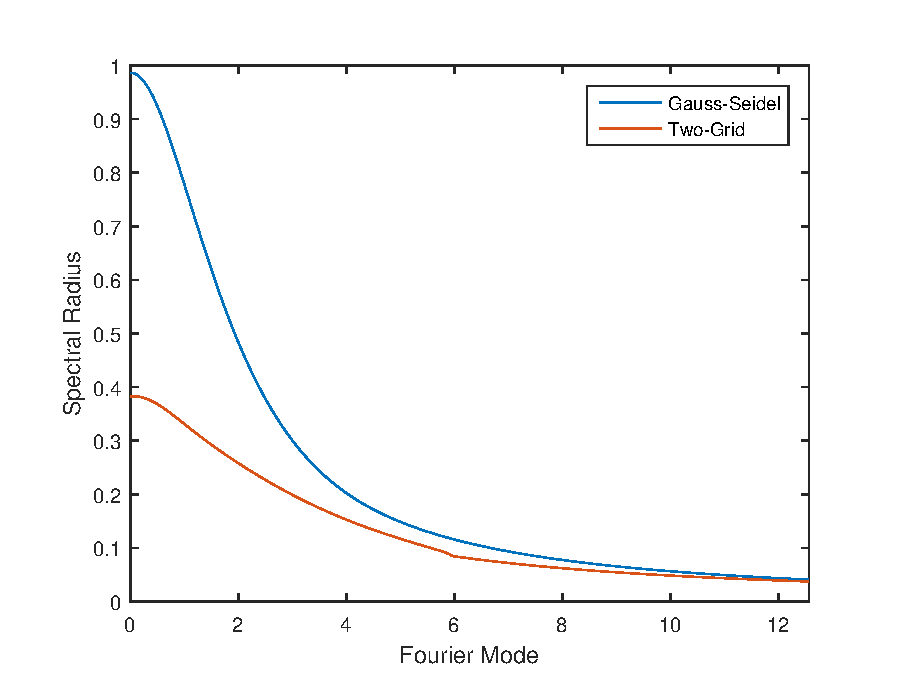
\includegraphics[width=0.485\textwidth]{images/P0_Fourier_69G.eps} \hfill
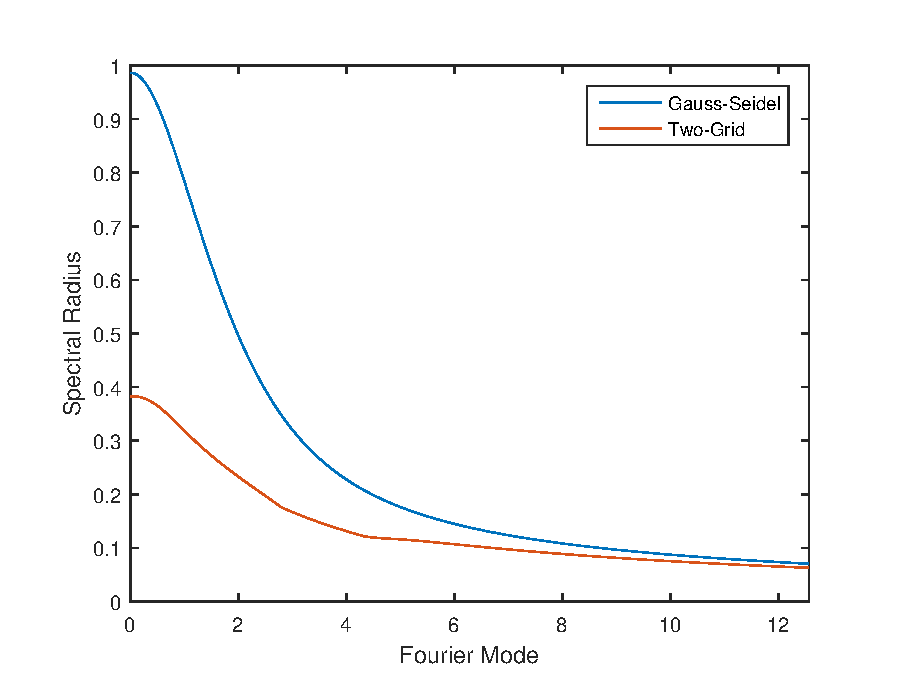
\includegraphics[width=0.485\textwidth]{images/P1_Fourier_69G.eps}
}
\end{frame}
%---------------------------
%%%%%%%%%%%%%%%%%%%%%%%%%%%%%%%%%%%%%%%%%%%%%%%%%%%%%%%%%%%%%%%%%%%%%%%%%%%%%%%%%%%%%%%%%%%%%%
%
%
\section{Proposed Work and Current Status}
\subsection{}
\begin{frame}[t]\frametitle{Proposed Work}\vspace{-0.2cm}
\begin{block}{POLYFEM}{\footnotesize
\begin{enumerate}
	\item Analyze the 2D linear polygonal basis functions for use in DGFEM transport calculations
	\item Perform the same analysis with the quadratic serendipity basis functions
	\item Determine the effects of numerical integration on highly-distorted polygonal elements
	\item Perform analysis on benchmark cases using polygonal meshes (including AMR)
\end{enumerate}}
\end{block}
\begin{block}{MIP DSA}{\footnotesize
\begin{enumerate}
	\item Analyze the 2D polygonal basis functions with MIP DSA preconditioning through Fourier/numerical analysis
	\item Analyze the effects of AMR with polygonal basis functions on the MIP DSA PCG iteration counts (with and without bootstrapping)
	\item Extend the analysis of MIP DSA to arbitrary convex 3D polyhedra
	\item Implement MIP DSA in PDT using HYPRE
	\begin{enumerate}{\footnotesize
		\item Analyze the scalability of the method to high process counts
		\item Implement and perform analysis of two-grid acceleration
		\item Perform parametric studies on aggregation/partitioning factors - generate a performance model of MIP DSA with HYPRE
		\item Run realistic numerical experiments - IM1 and reactor geometries
	}\end{enumerate}
\end{enumerate}}
\end{block}
\end{frame}
\subsection{}
%---------------------------
\setbeamerfont{frametitle}{size=\small}
\begin{frame}[t]\frametitle{2D Exactly-Linear Transport Solutions - mean value coordinates}
\begin{block}{}
\begin{equation*}
\begin{aligned}
\mu \frac{\partial  \psi}{\partial x} + \eta \frac{\partial  \psi}{\partial y} + \sigma_t \psi &= Q(x,y,\mu,\eta) \\
\psi (x,y,\mu,\eta) = a x + b y + c \mu + d \eta + e& , \qquad  \phi (x,y) = 2 \pi \left(   a x + b y  + e  \right)
\end{aligned}
\end{equation*}
\end{block}
\centering
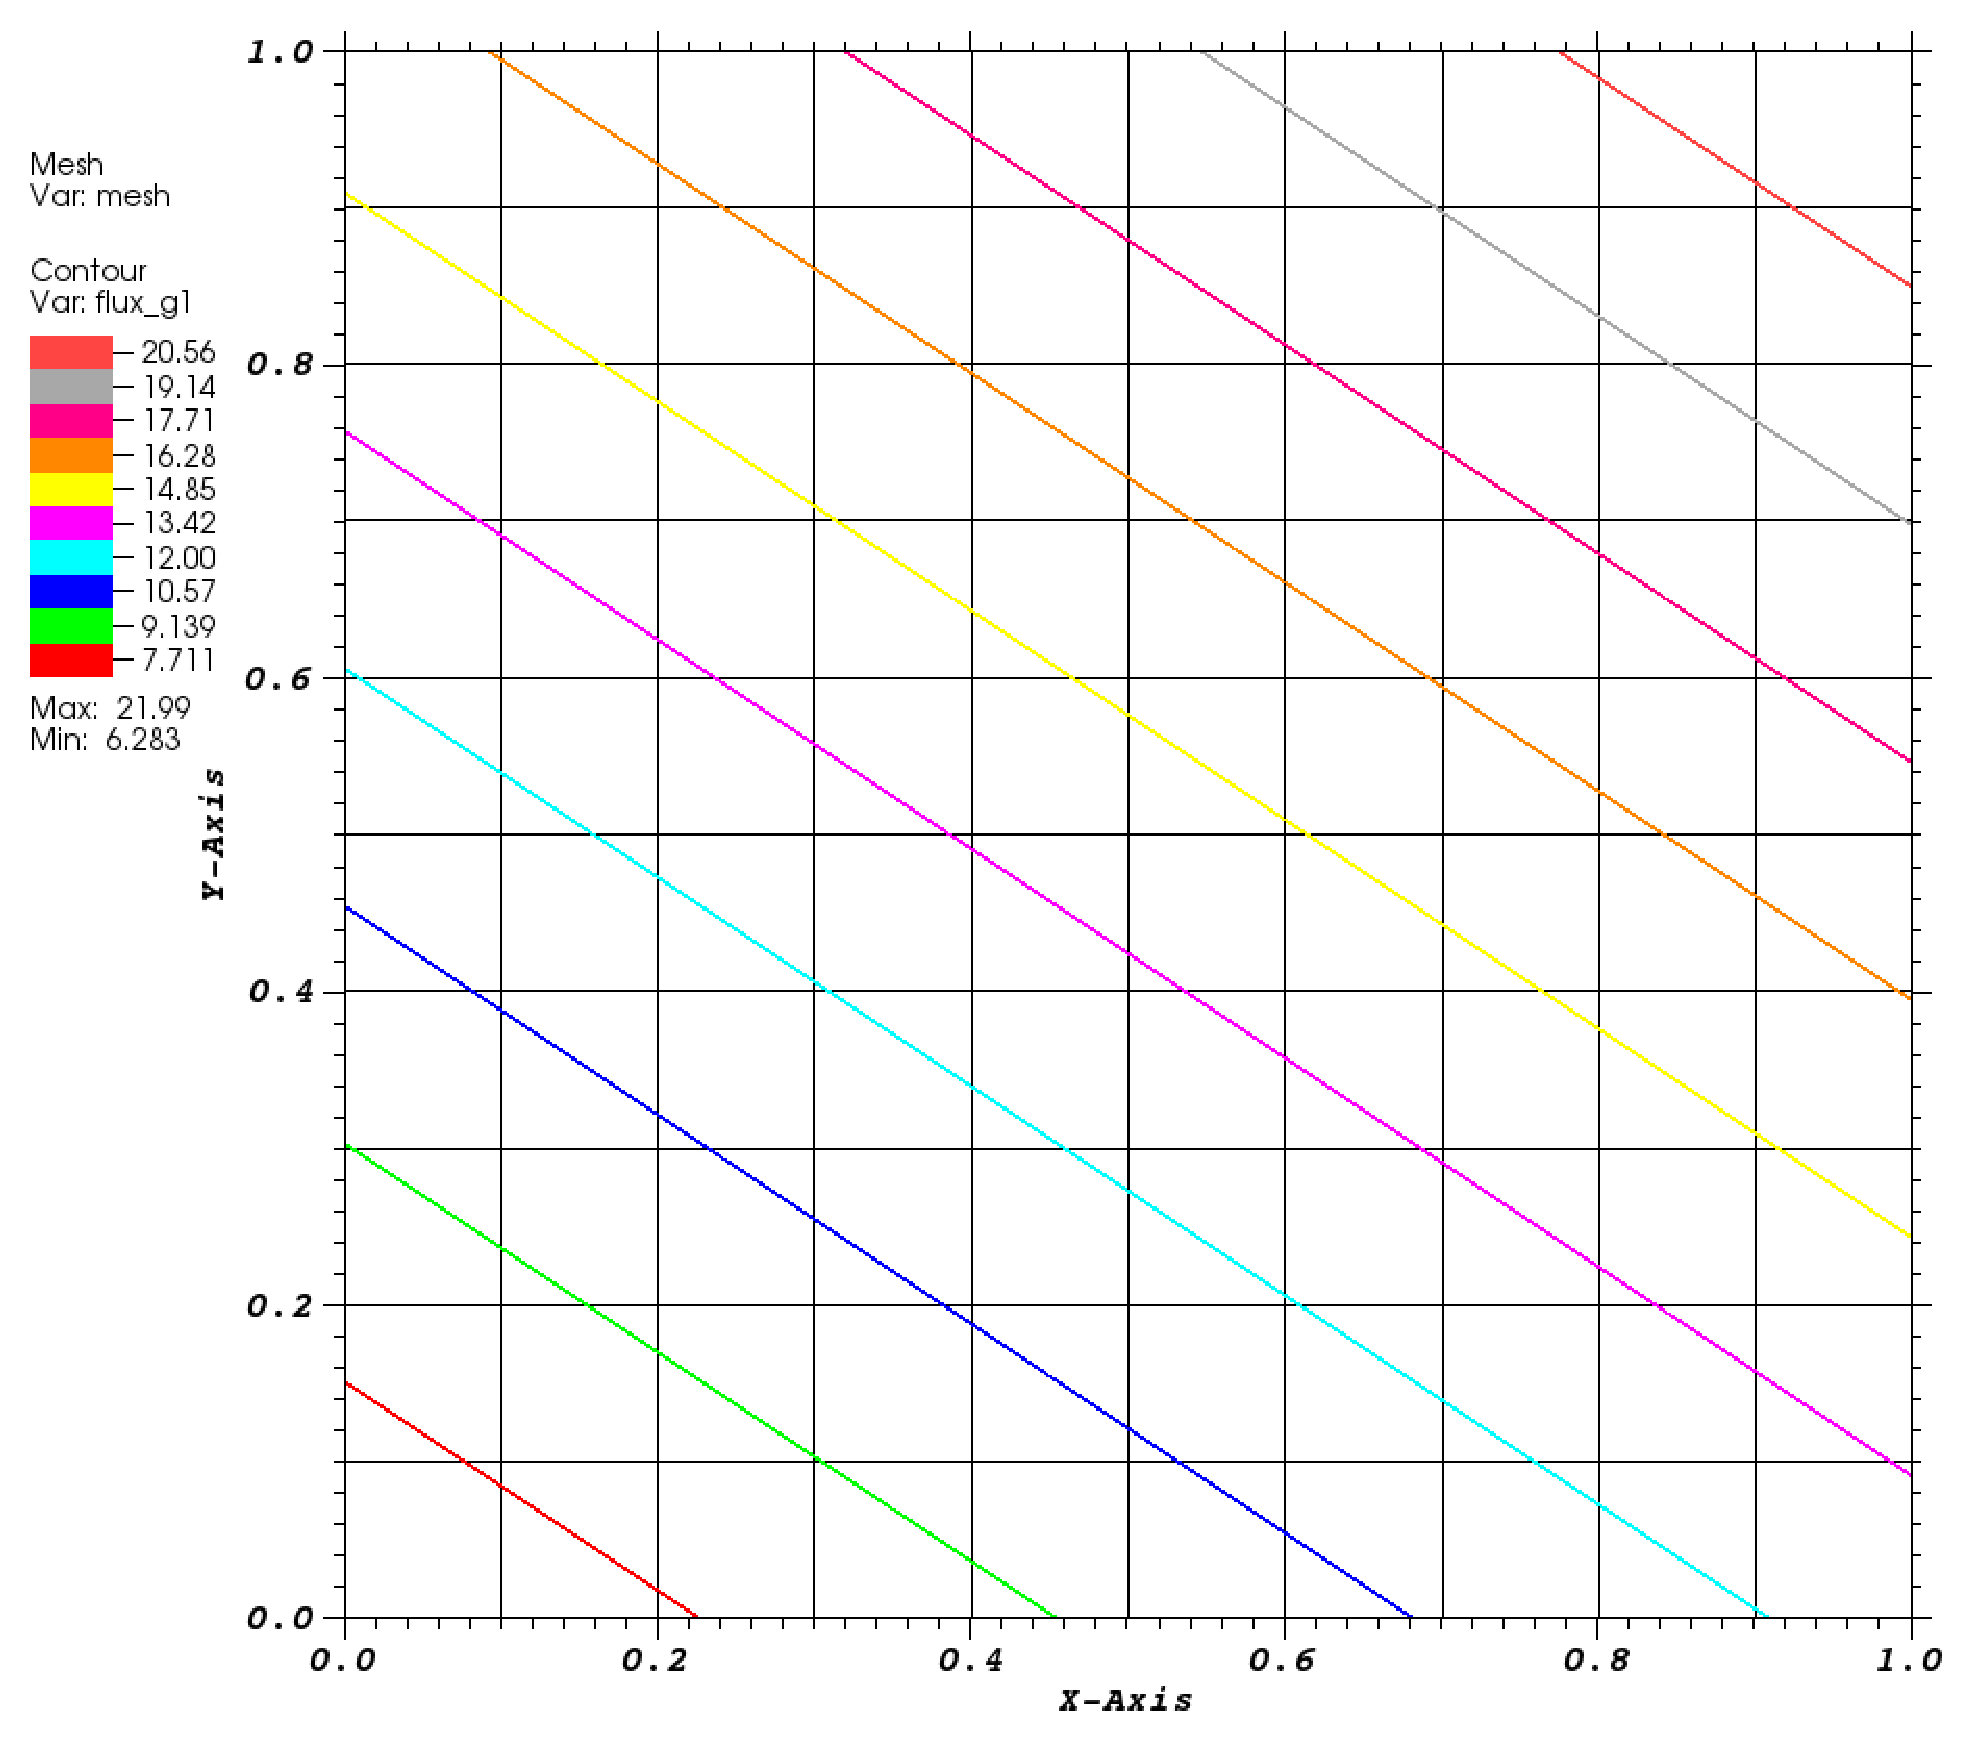
\includegraphics[width=0.25\textwidth]{images/cart_MV_k1.eps} 
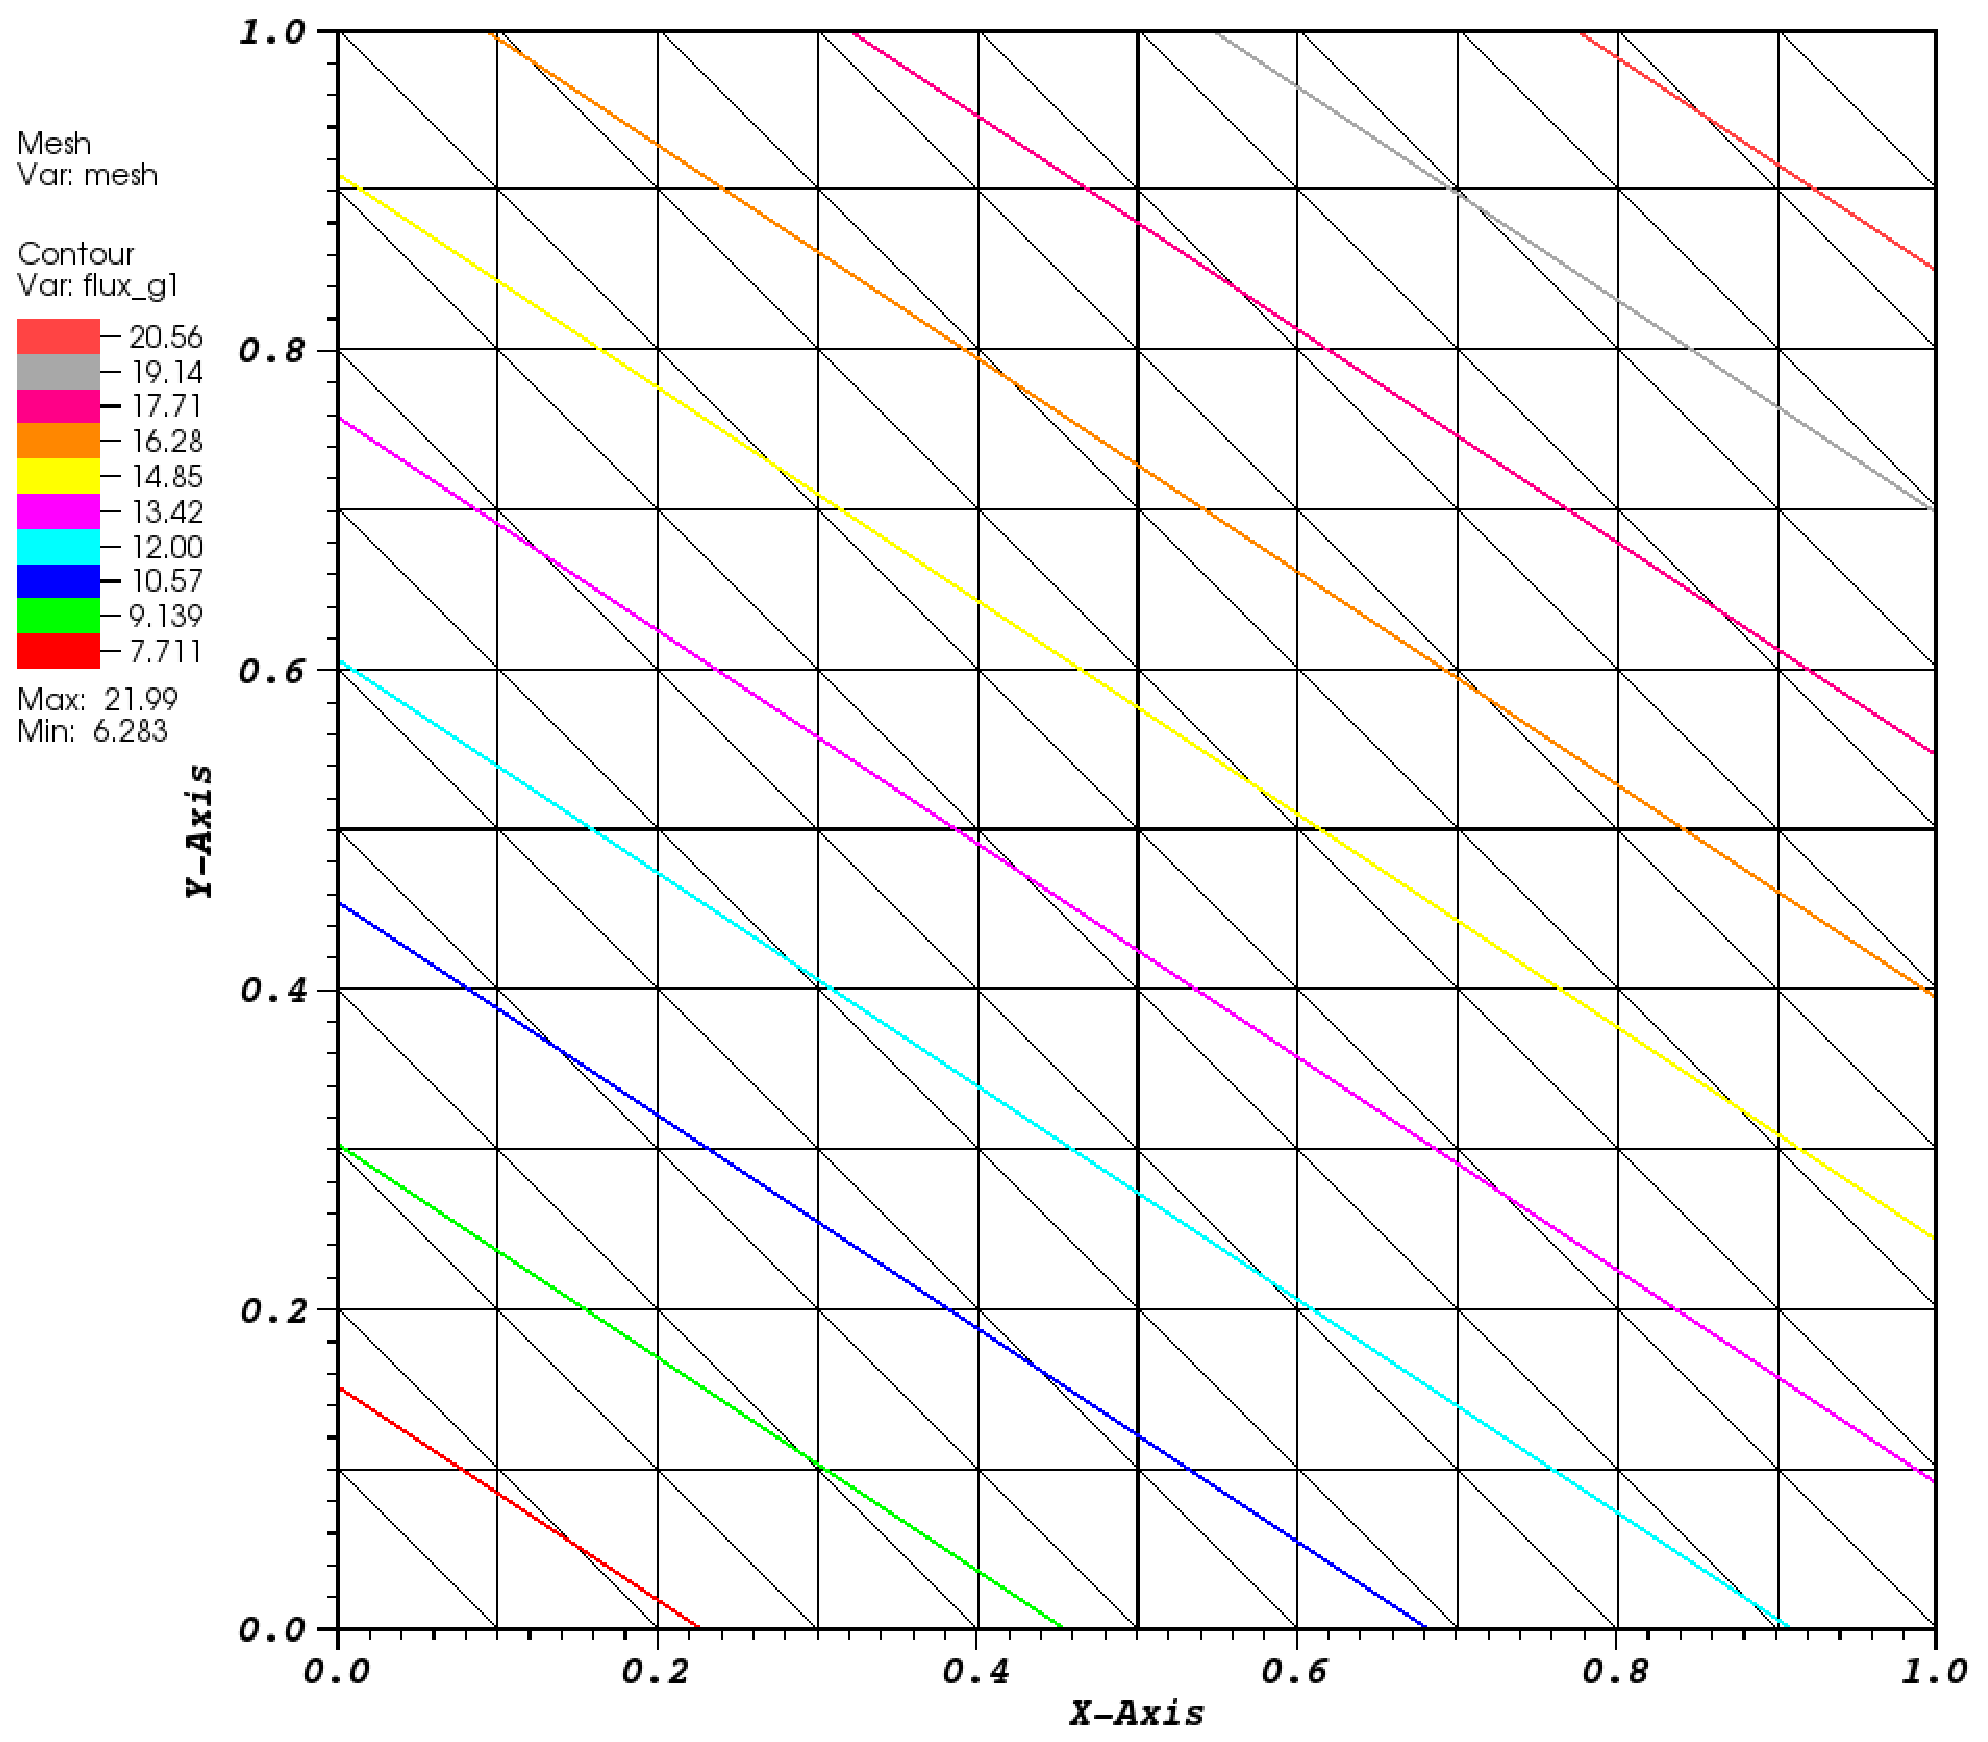
\includegraphics[width=0.25\textwidth]{images/tri_MV_k1.eps} 
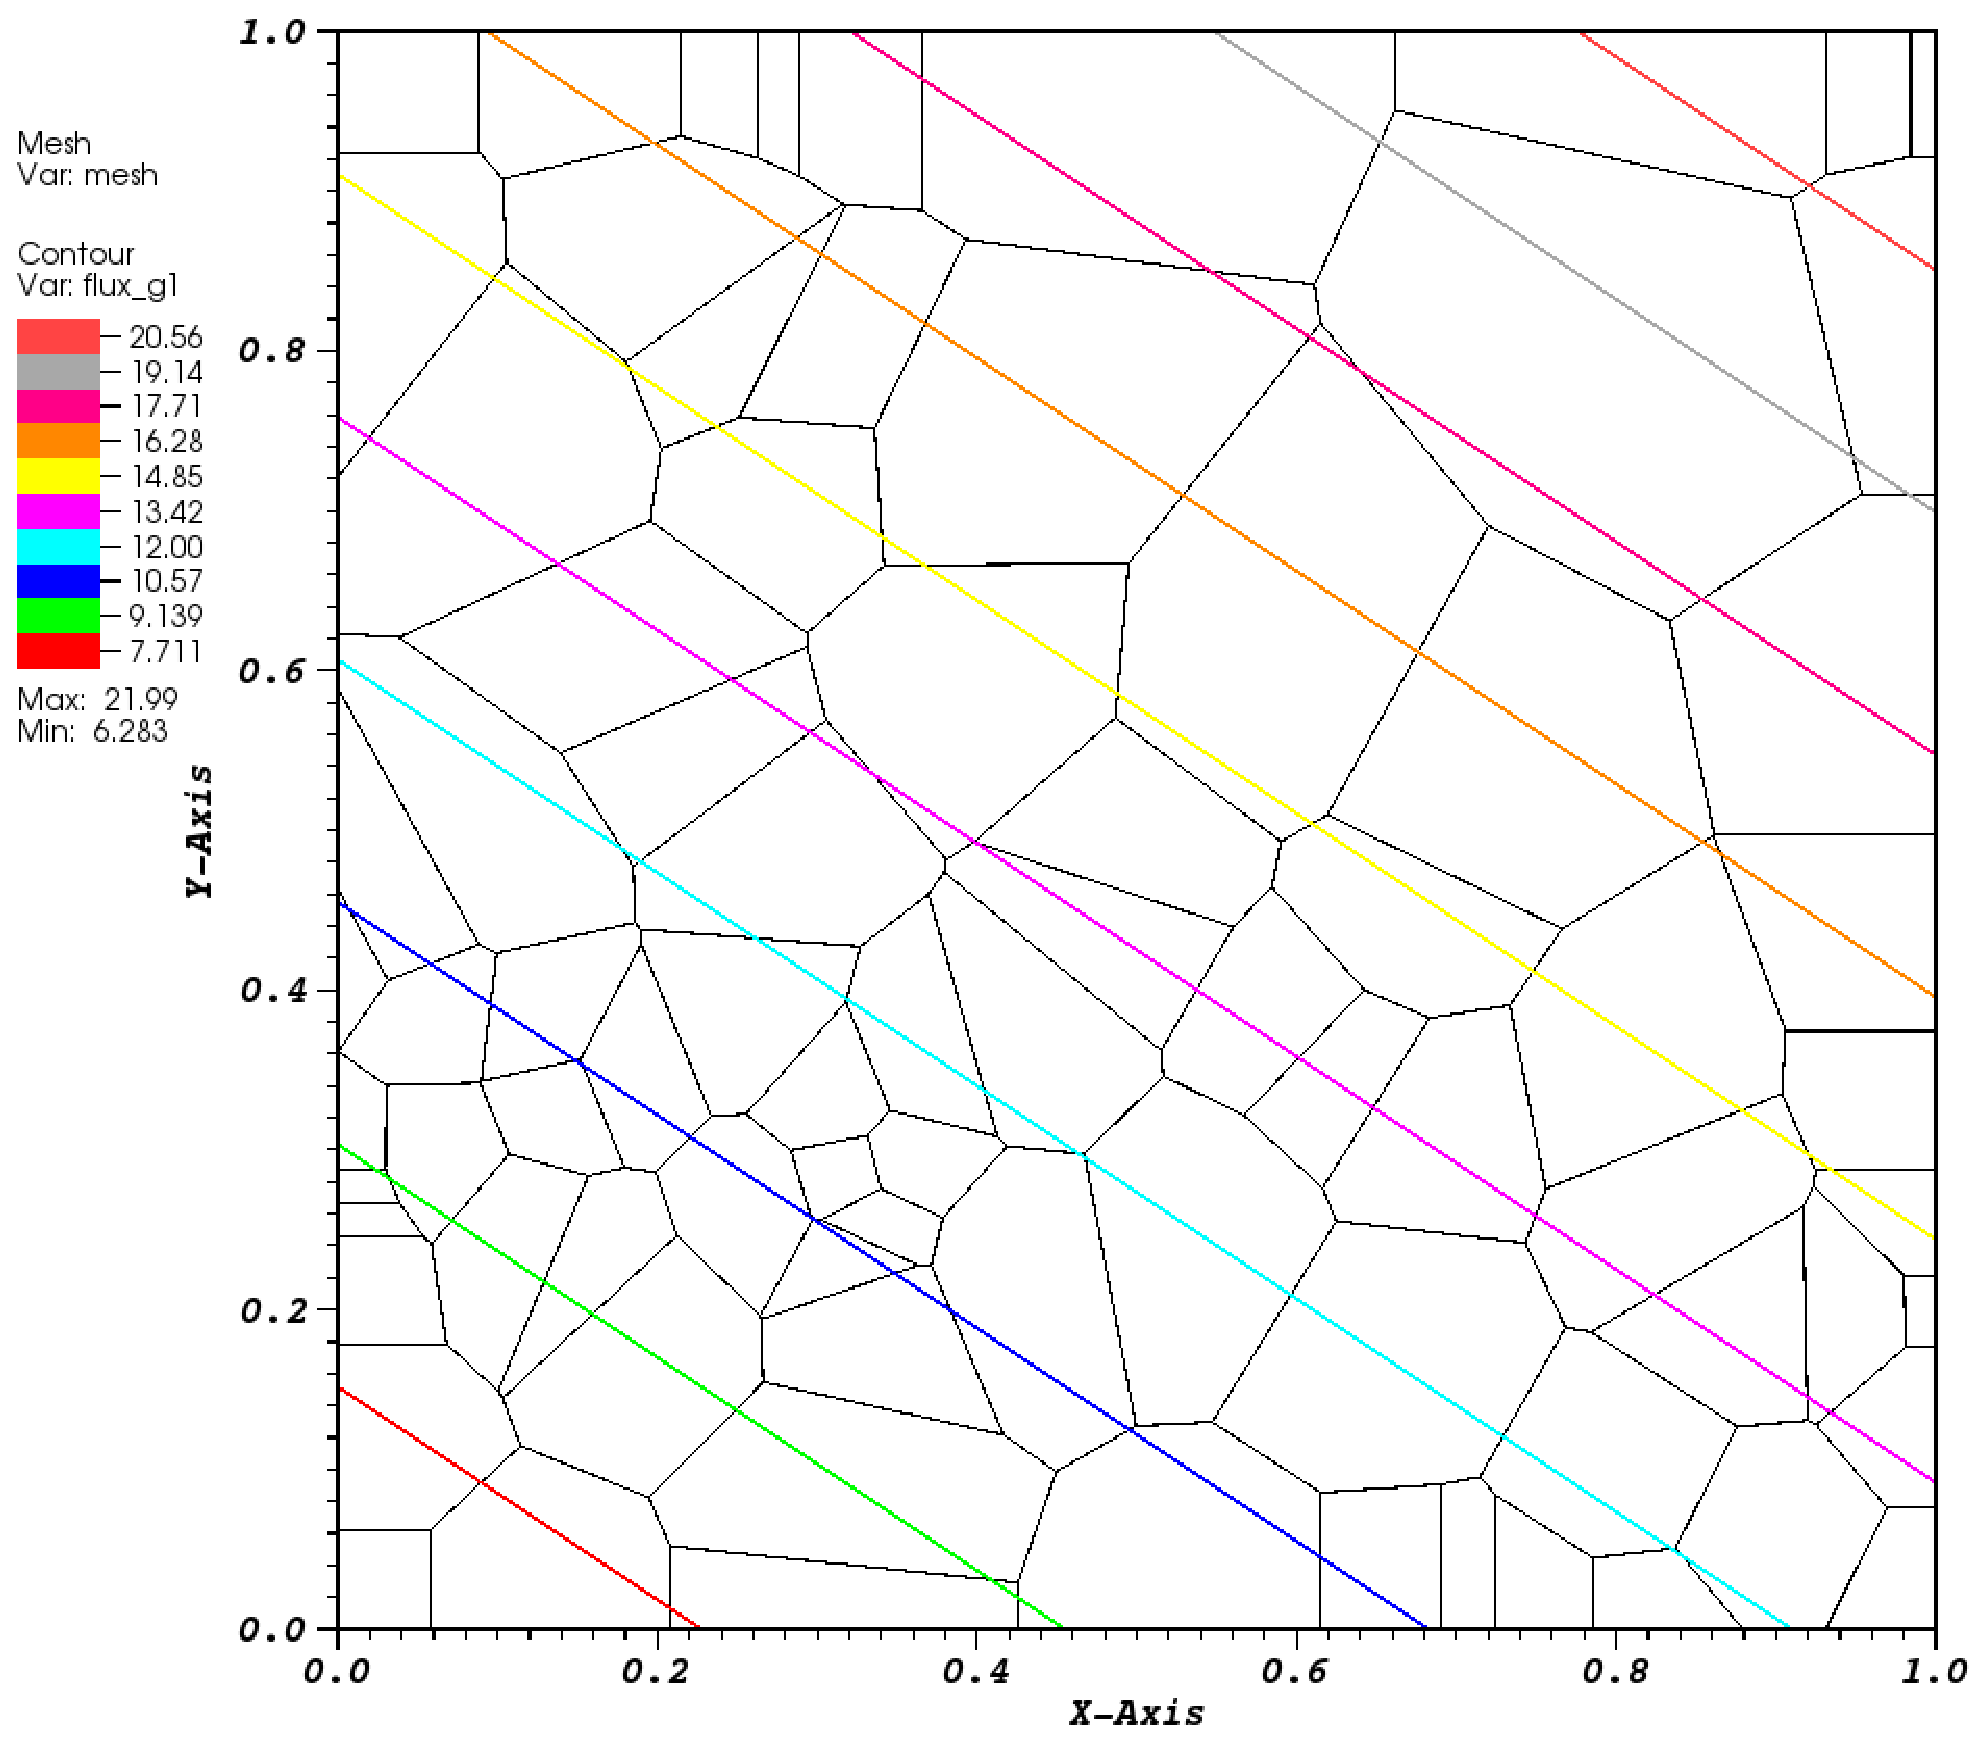
\includegraphics[width=0.25\textwidth]{images/shes_poly_MV_k1.eps} 
\vspace{0.2cm}
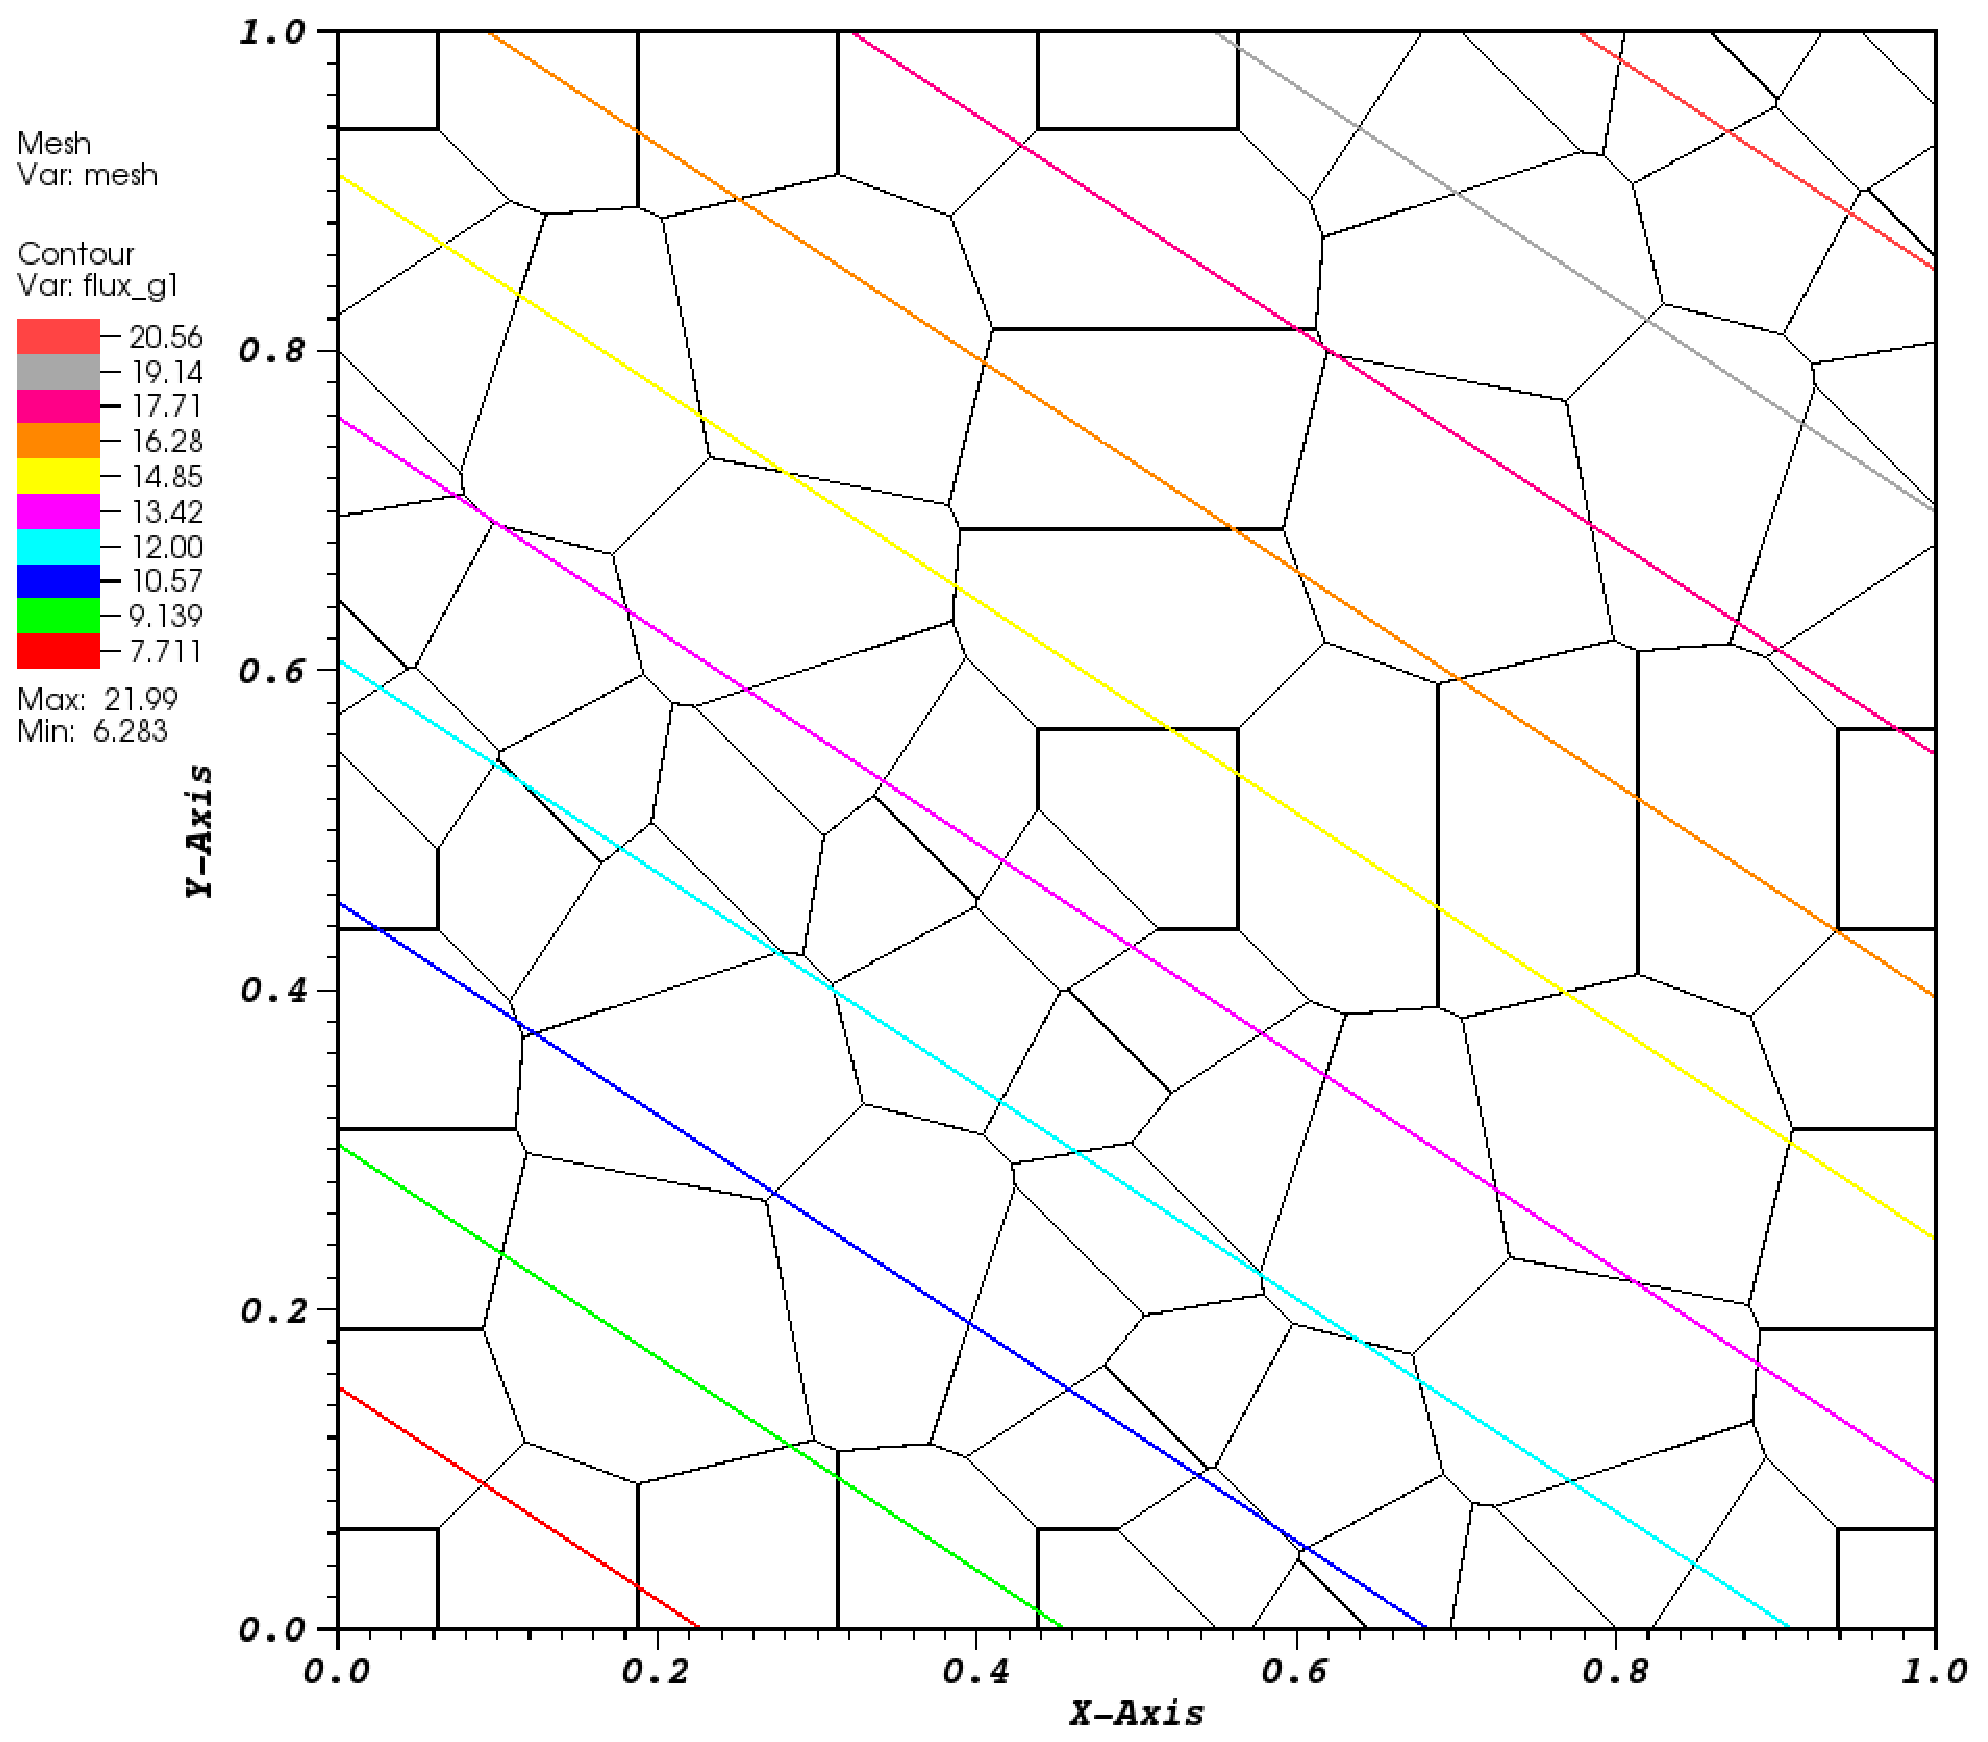
\includegraphics[width=0.25\textwidth]{images/smooth_poly_MV_k1.eps} 
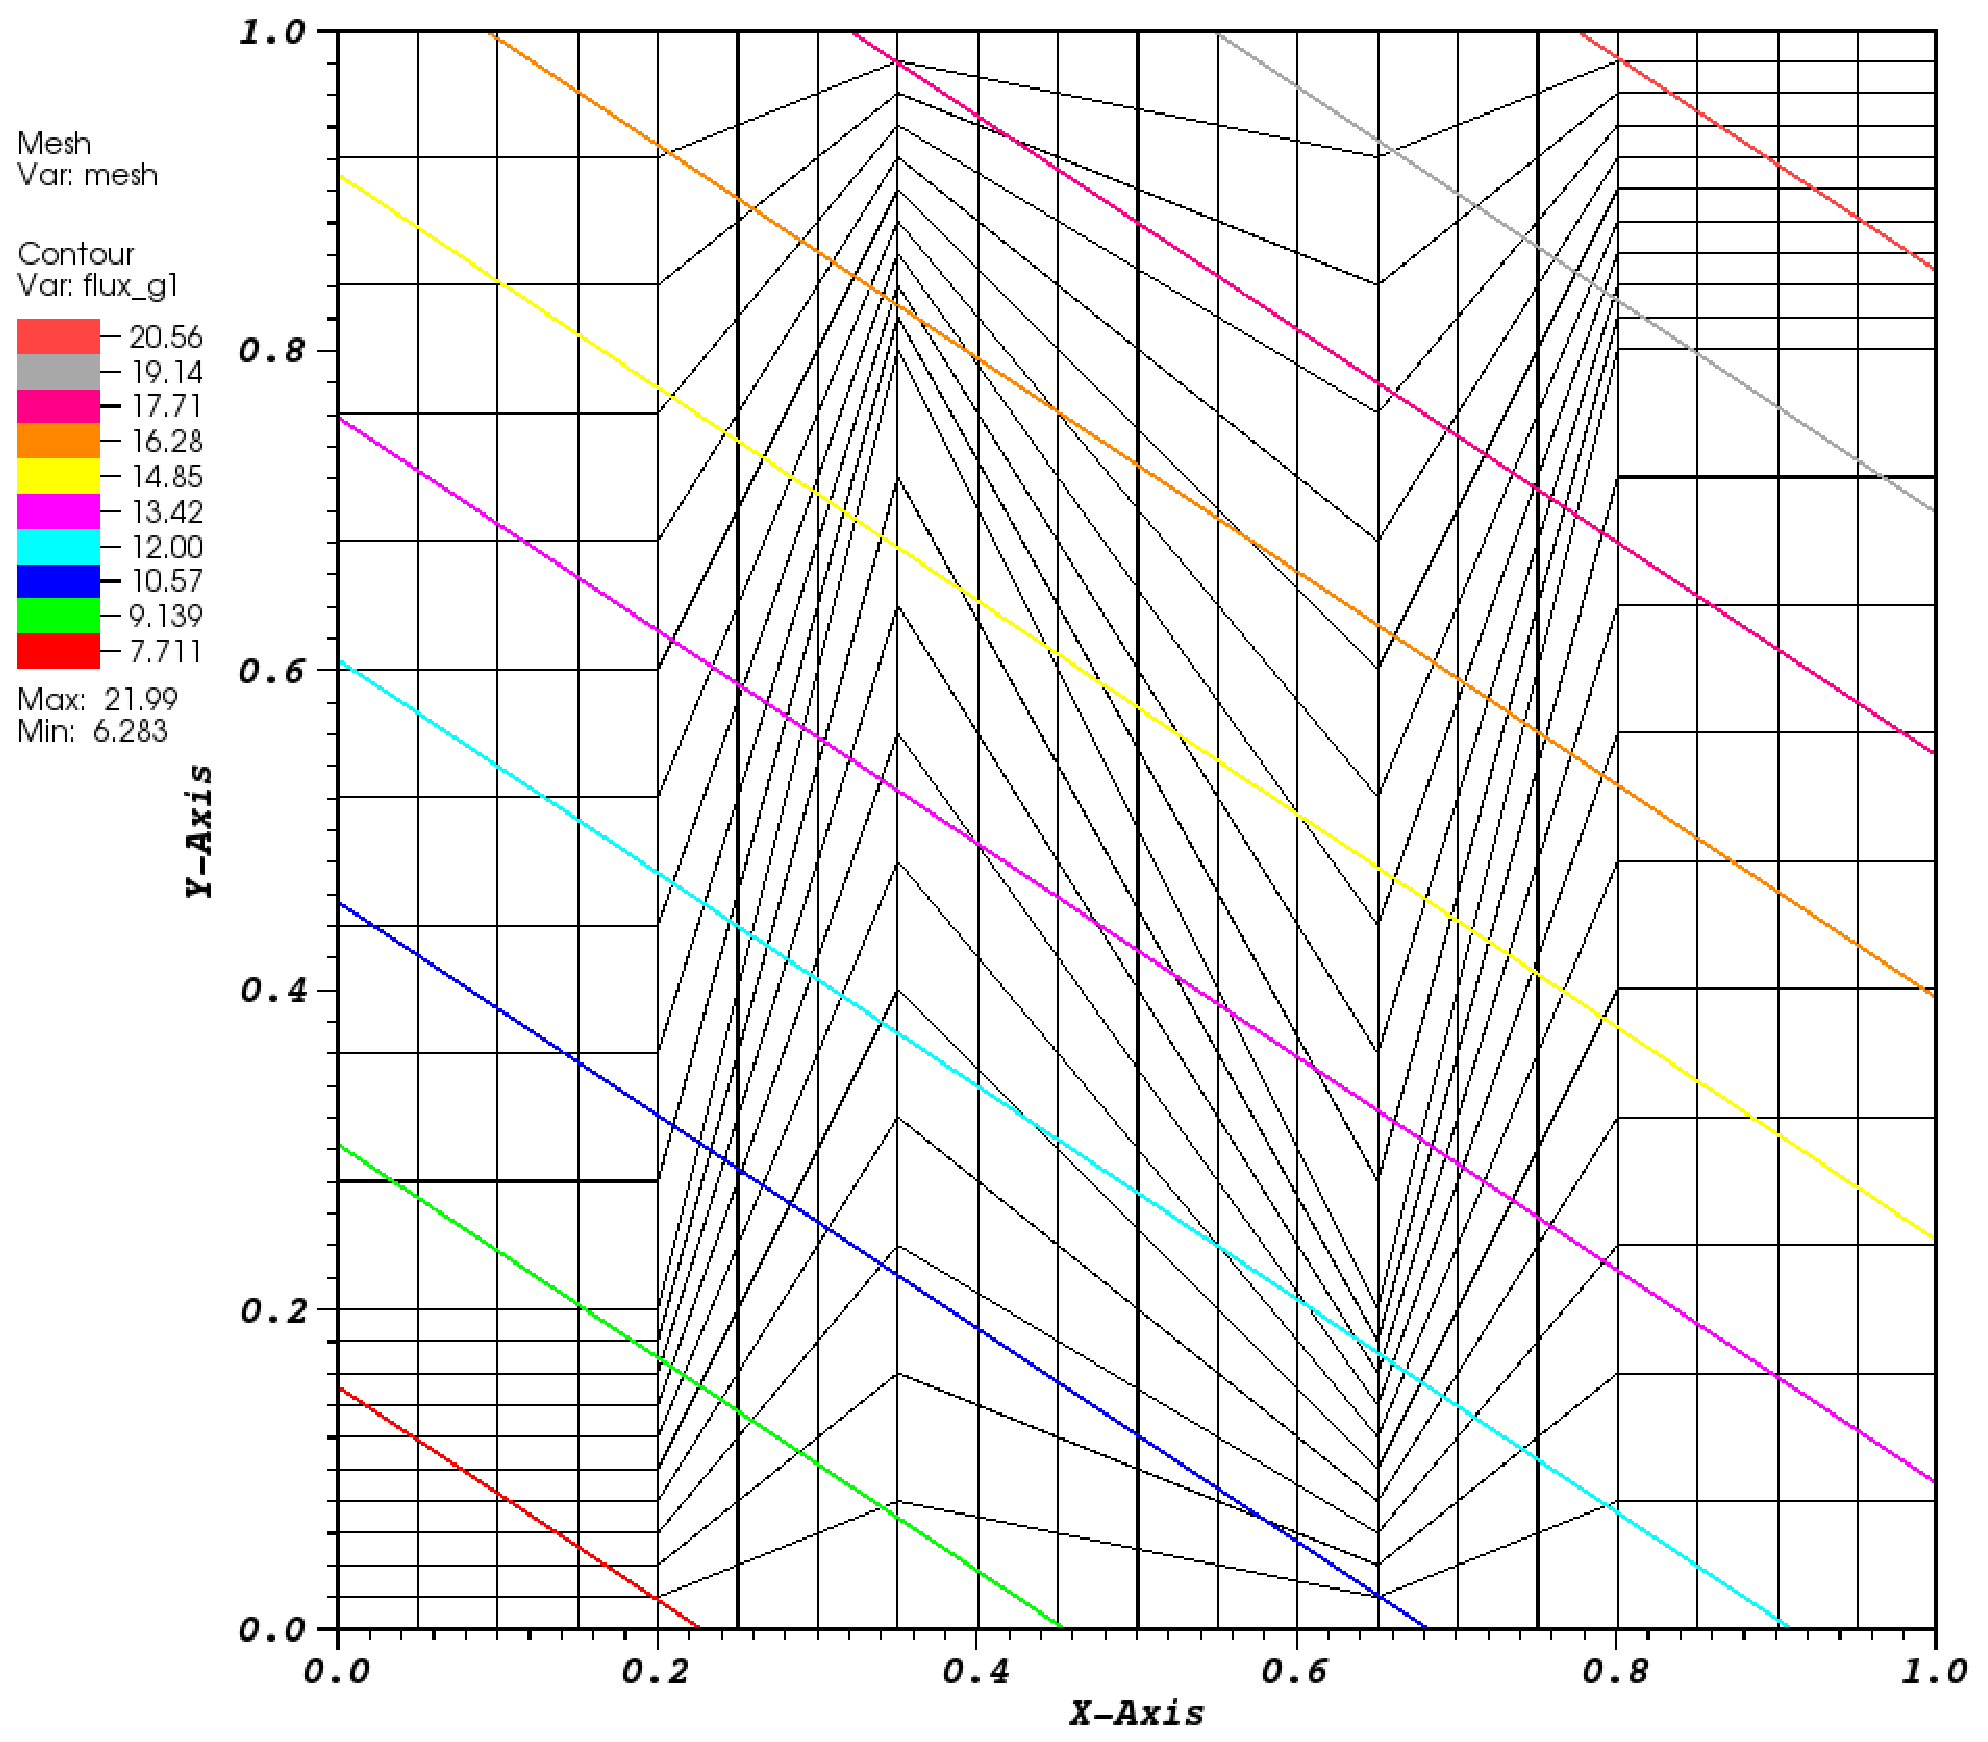
\includegraphics[width=0.25\textwidth]{images/z_quad_MV_k1.eps}
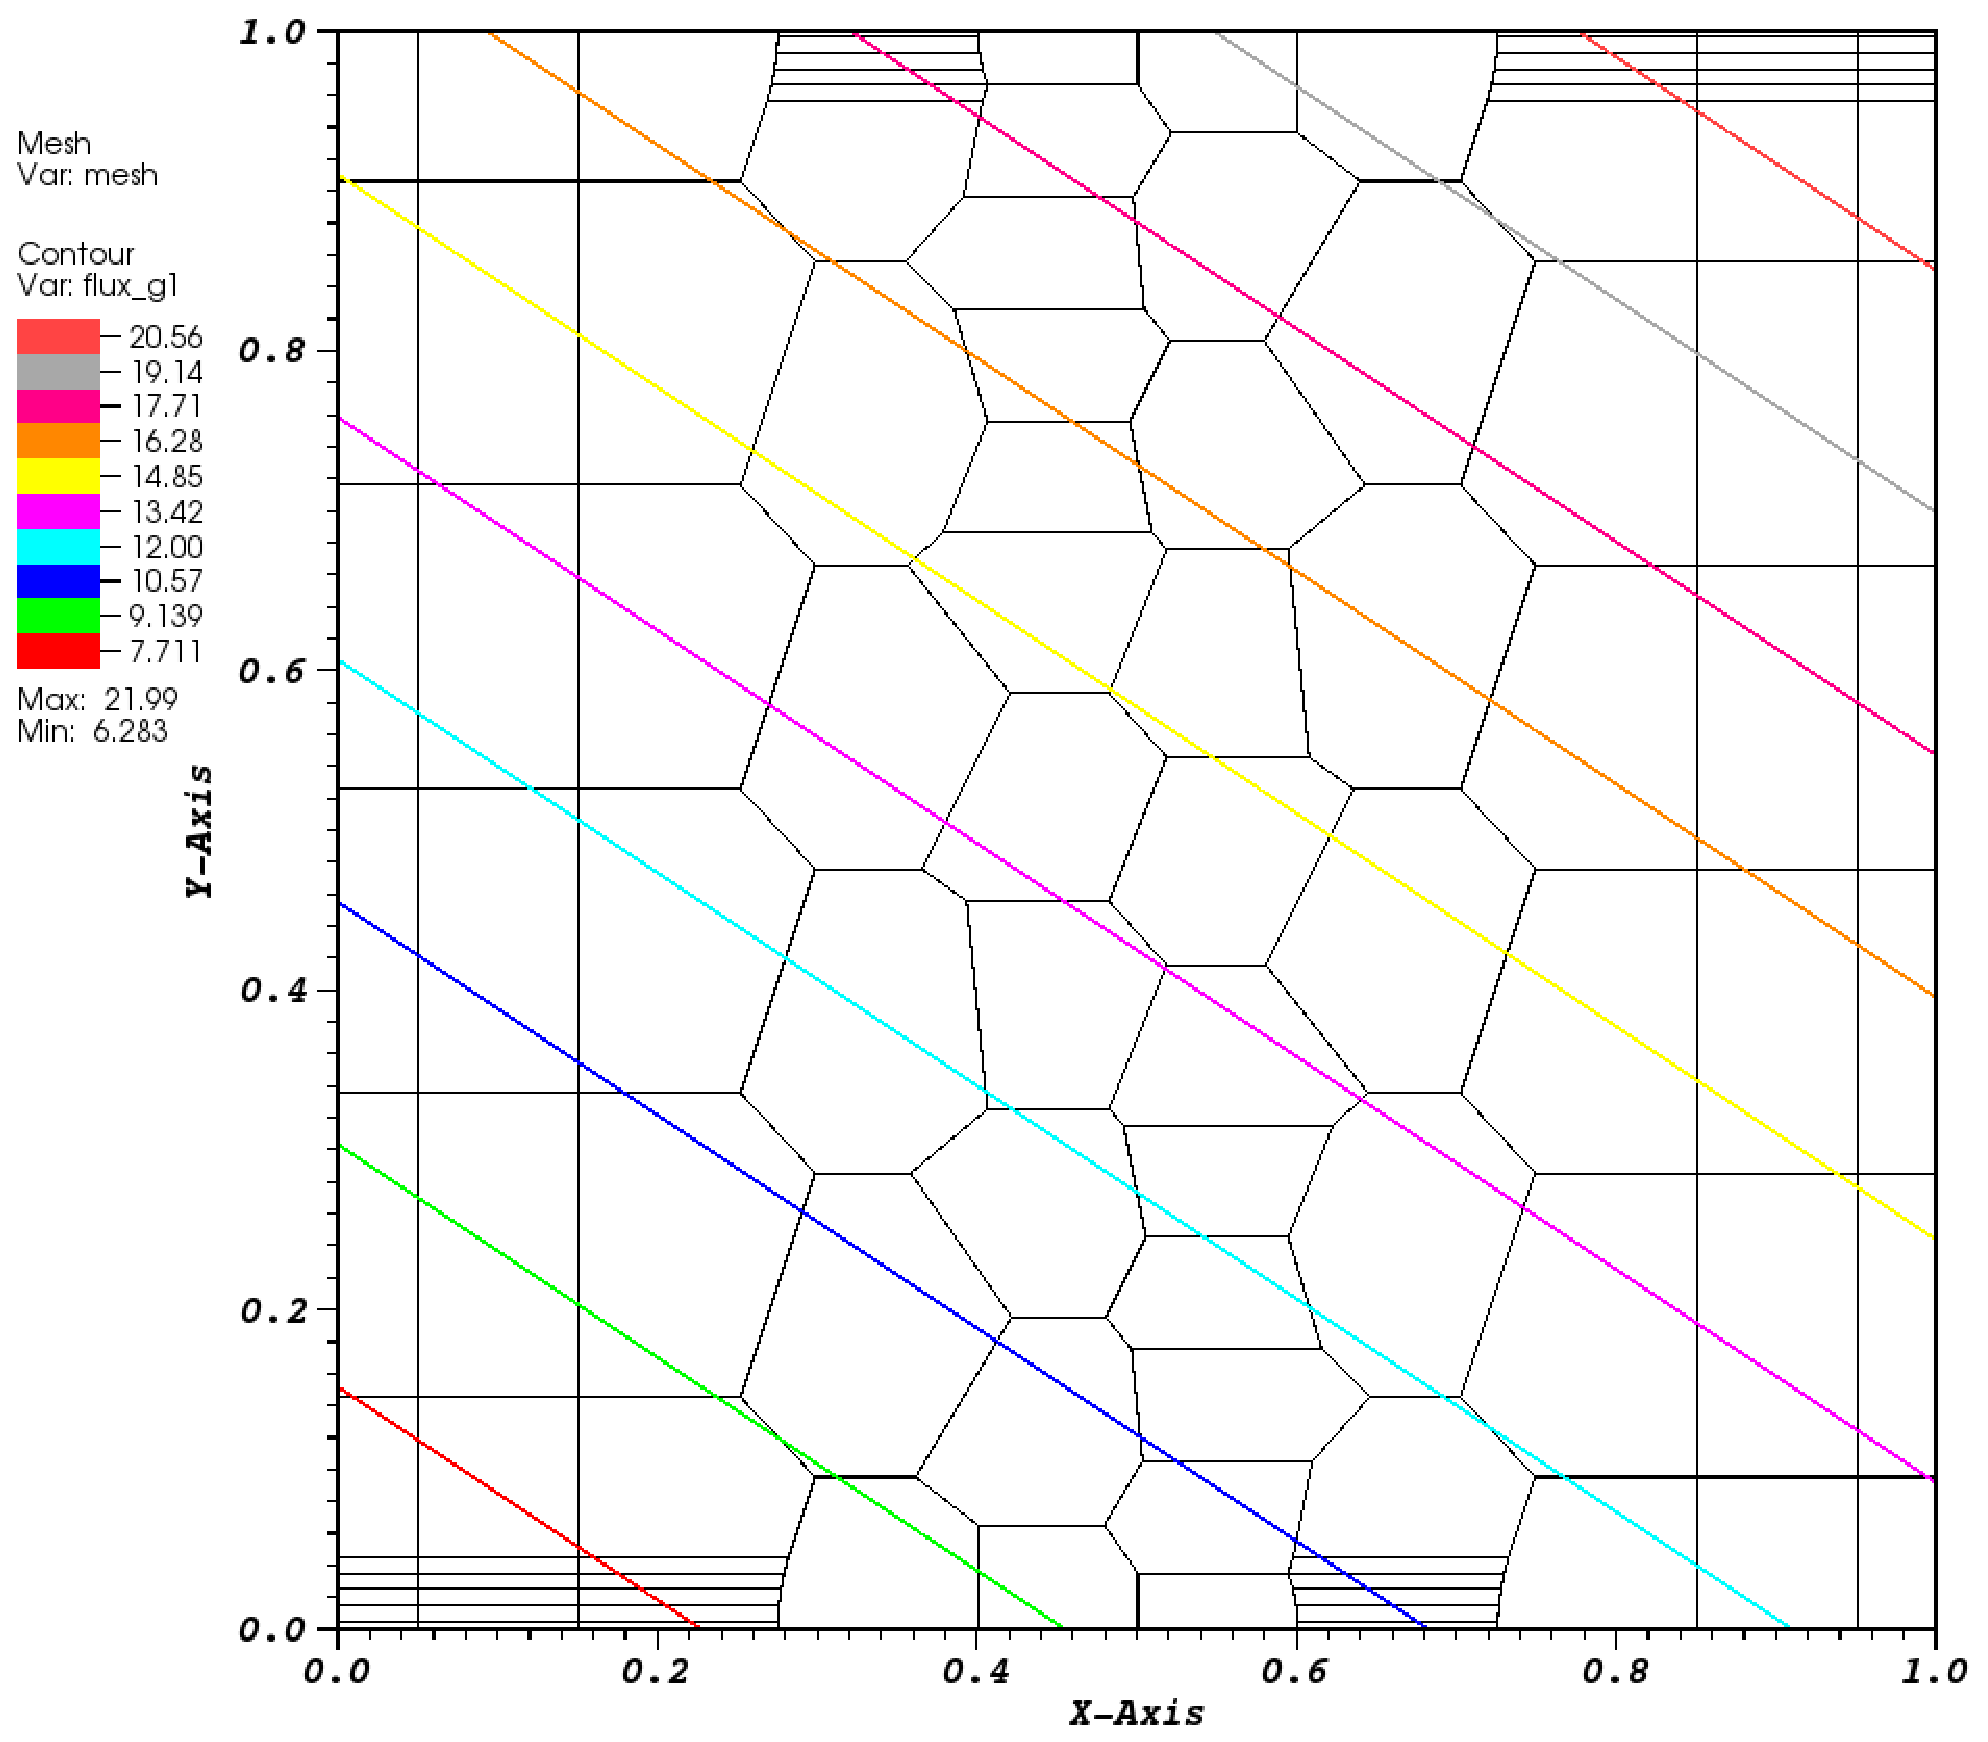
\includegraphics[width=0.25\textwidth]{images/z_poly_MV_k1.eps}
\end{frame}
%---------------------------
\setbeamerfont{frametitle}{size=\small}
\begin{frame}[t]\frametitle{Convergence rates using MMS for the 2D polygonal basis functions}
\only<1-3>{
\begin{block}{}
\begin{equation*}
\begin{aligned}
\psi (x,y) = \sin(\nu \frac{\pi x}{L_x}) \sin(\nu \frac{\pi y}{L_y}) \\
 \phi (x,y) = 2 \pi \sin(\nu \frac{\pi x}{L_x}) \sin(\nu \frac{\pi y}{L_y})
\end{aligned}
\end{equation*}
\end{block}
}
\vspace{0.4cm}
\begin{columns}
\column{0.40\textwidth}
\centering
\only<1>{
{}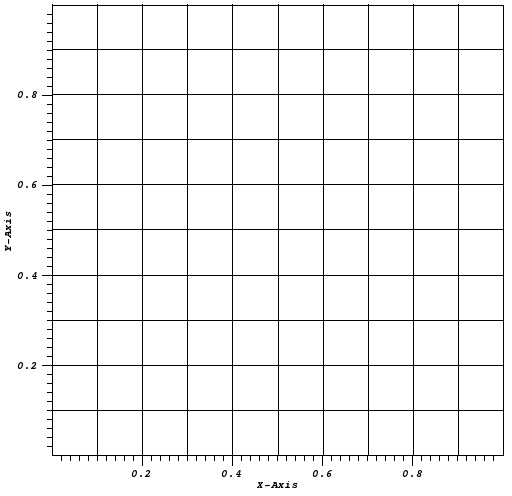
\includegraphics[width=0.8\columnwidth]{images/cart_mesh.jpg}
}
\only<2>{
{}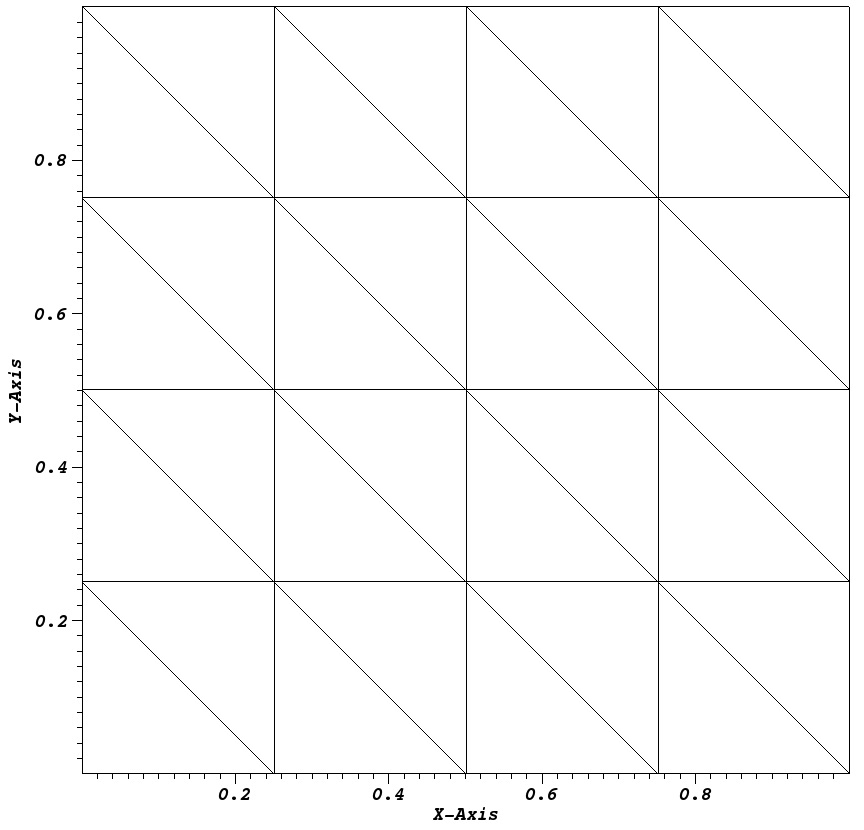
\includegraphics[width=0.8\columnwidth]{images/tri_mesh.jpg}
}
\only<3>{
{}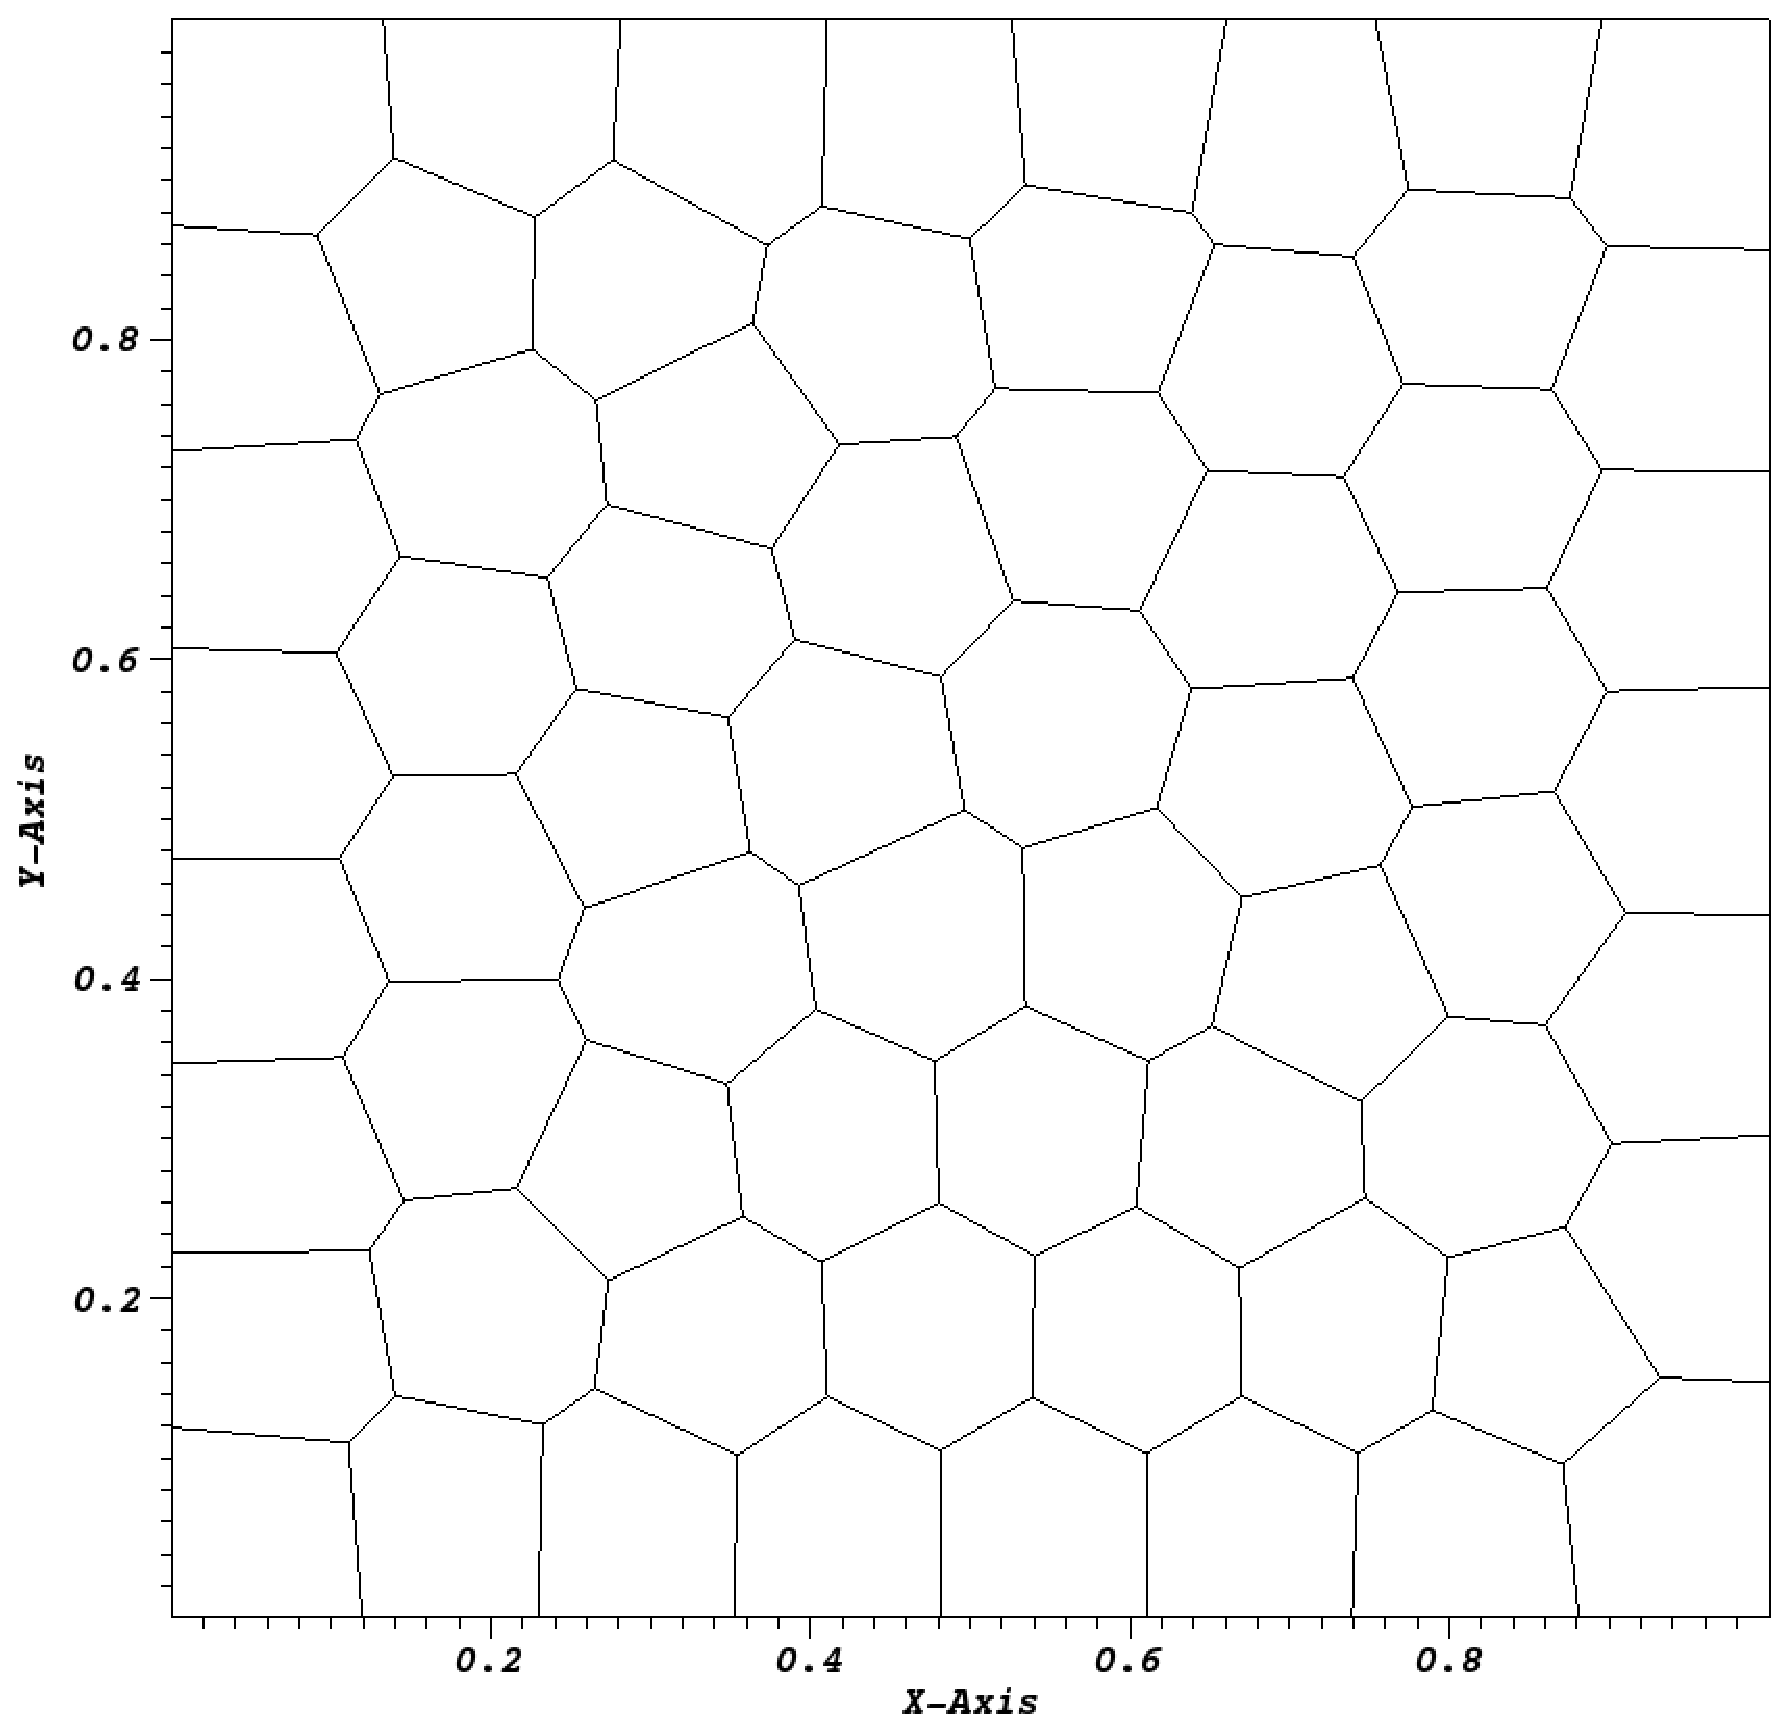
\includegraphics[width=0.8\columnwidth]{images/PolyMesh_mesh.eps}
}
\column{0.60\textwidth}
\centering
\only<1>{
{}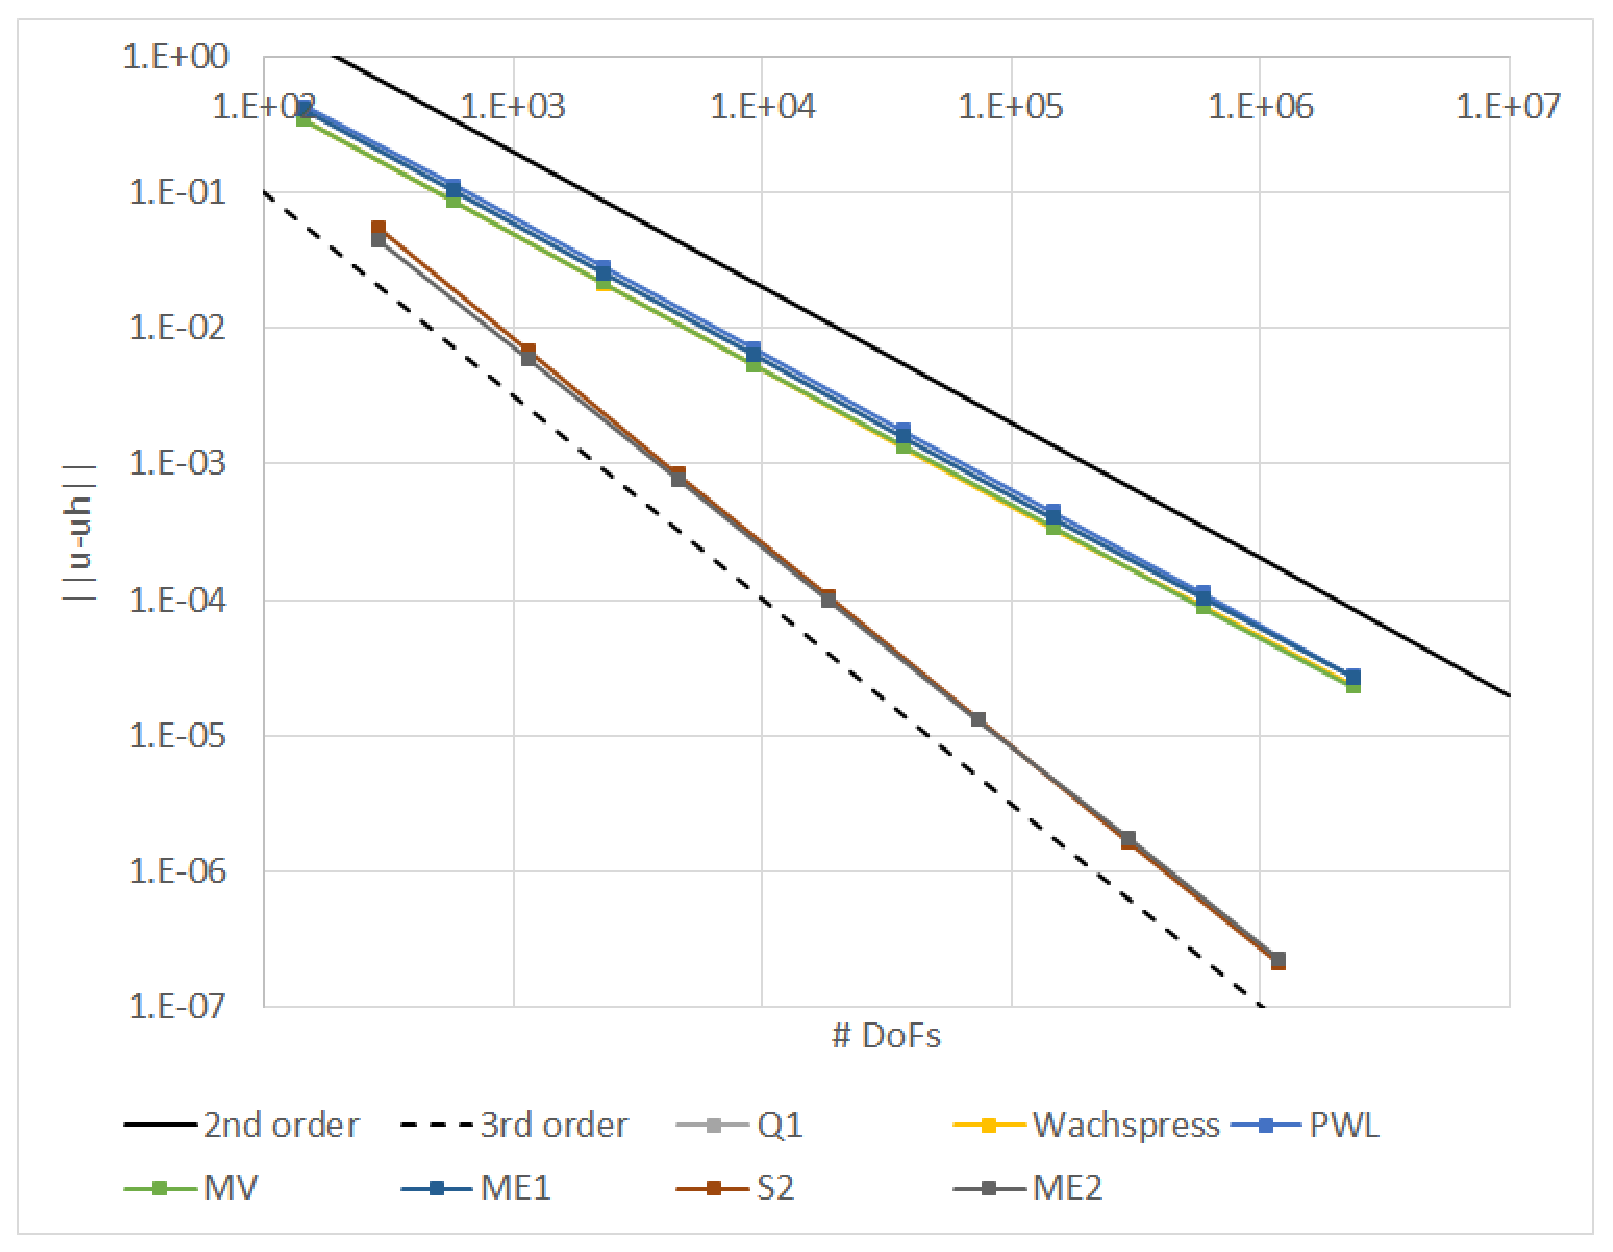
\includegraphics[width=0.9\columnwidth]{images/cart_err.eps}
}
\only<2>{
{}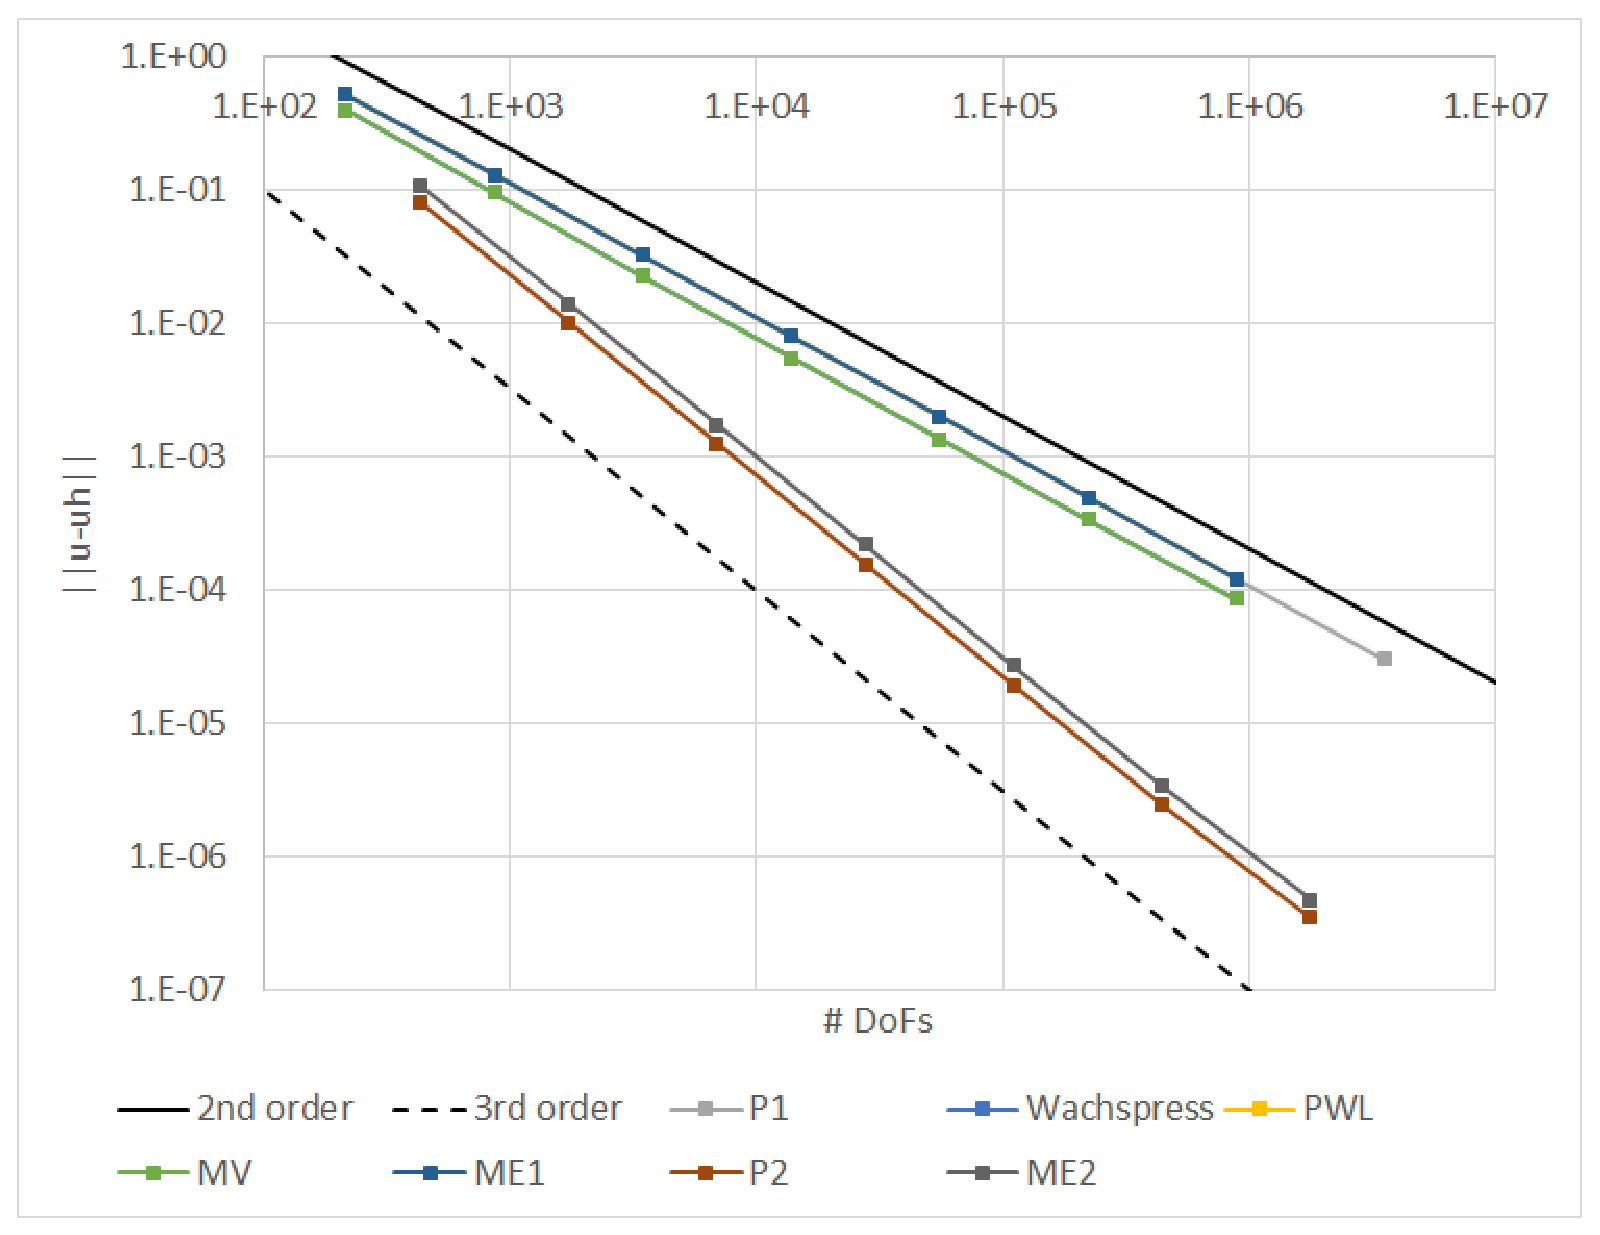
\includegraphics[width=0.9\columnwidth]{images/tri_err.eps}
}
\only<3>{
{}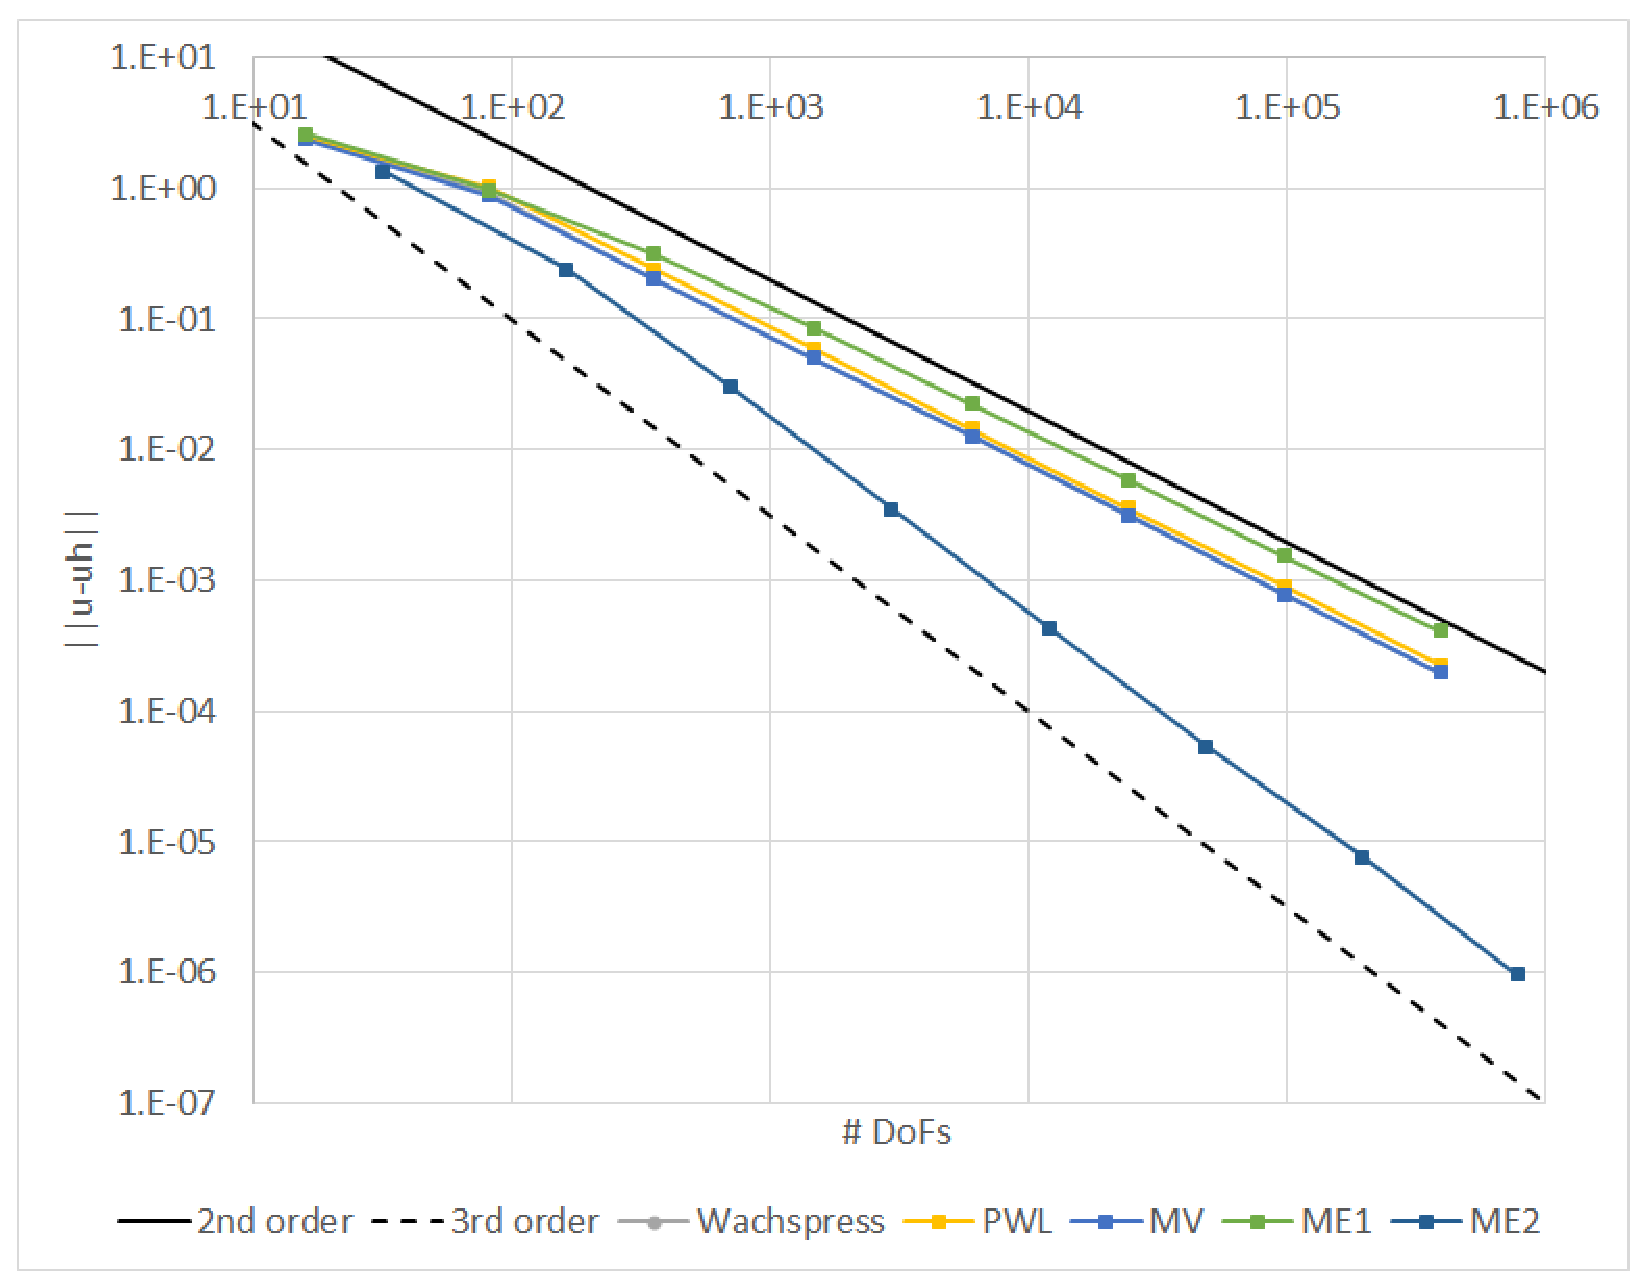
\includegraphics[width=0.9\columnwidth]{images/poly_err.eps}
}
\end{columns}
\end{frame}
%---------------------------
\begin{frame}[t]\frametitle{Convergence rates using MMS and AMR for the 2D polygonal basis functions}
\begin{block}{}
\begin{equation*}
\begin{aligned}
\psi (x,y) = & x (L_x - x) y (L_y - y) \exp(-\frac{(x-x_0)^2 + (y-y_0)^2}{\gamma}), \\ 
\phi (x,y) = 2 \pi & x (L_x - x) y (L_y - y) \exp(-\frac{(x-x_0)^2 + (y-y_0)^2}{\gamma})
\end{aligned}
\end{equation*}
\end{block}
\centering
{}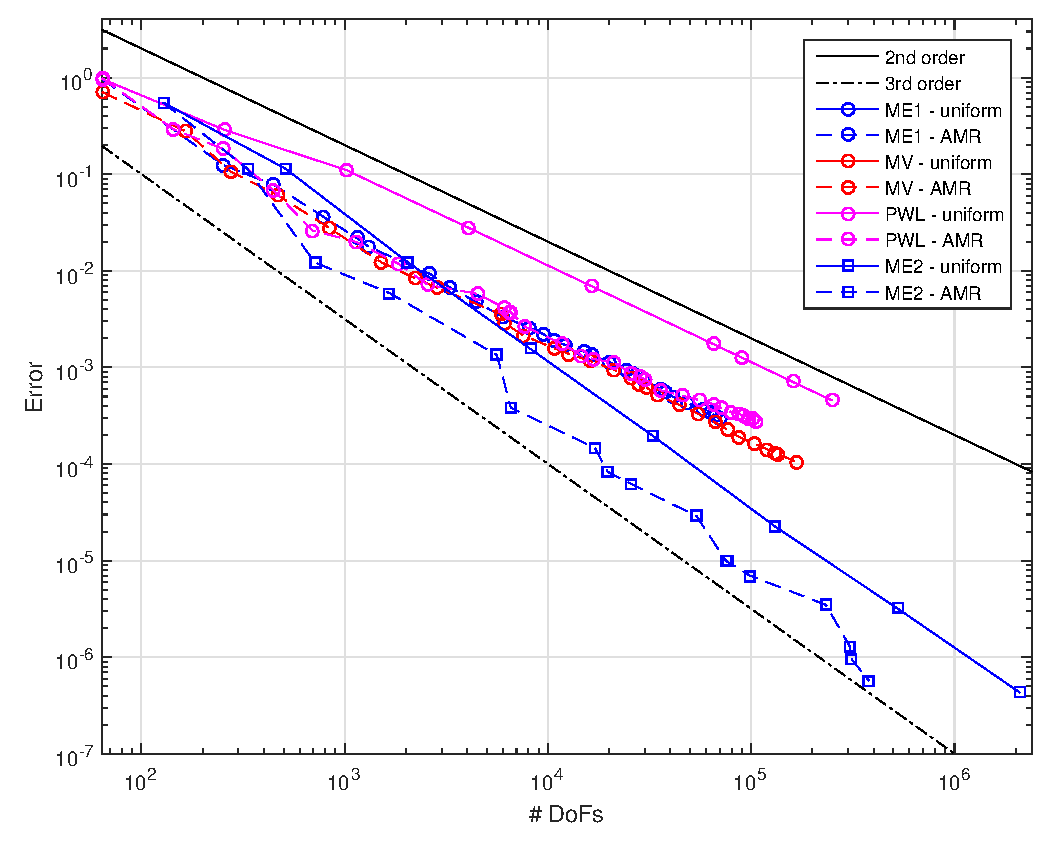
\includegraphics[width=0.55\columnwidth]{images/Transport_Gauss_2D_AMR_Error_Plot.eps}
\end{frame}
%---------------------------
\setbeamerfont{frametitle}{size=\footnotesize}
\begin{frame}[t]\frametitle{Linear ME cycle 15 (left) and quadratic ME cycle 08 (right)}
\begin{columns}
\column{0.50\textwidth}
\centering
{}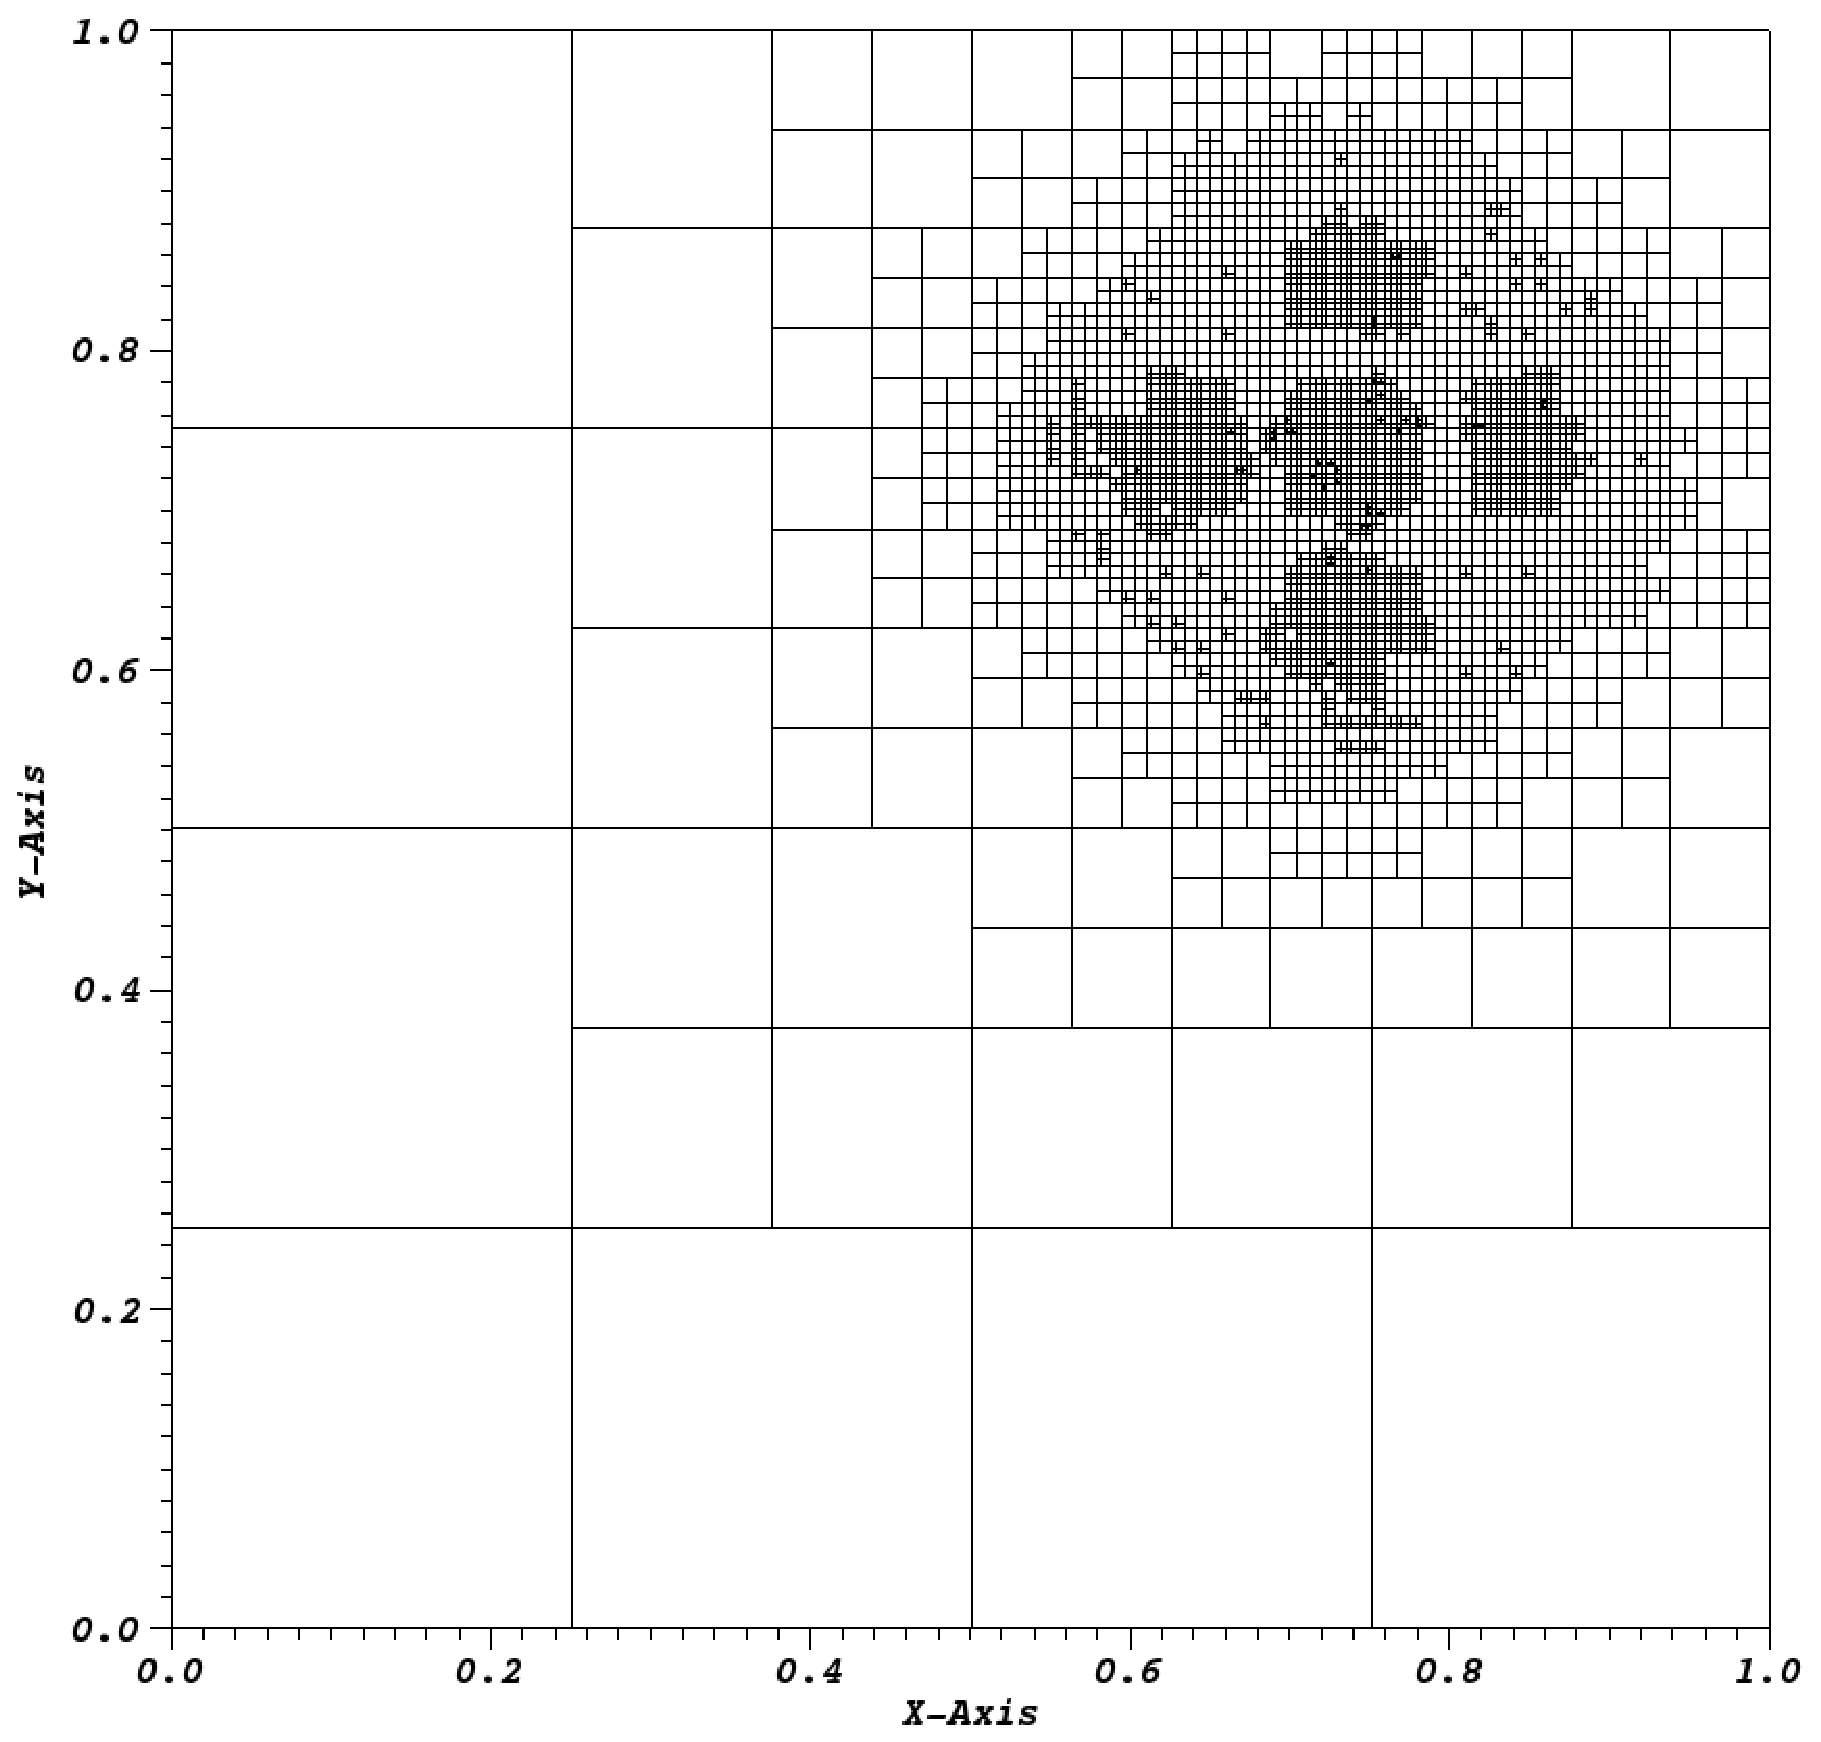
\includegraphics[width=0.70\columnwidth]{images/ME1_cart_Irr=1_tol=0.2_cyc15_mesh.eps} \\
{}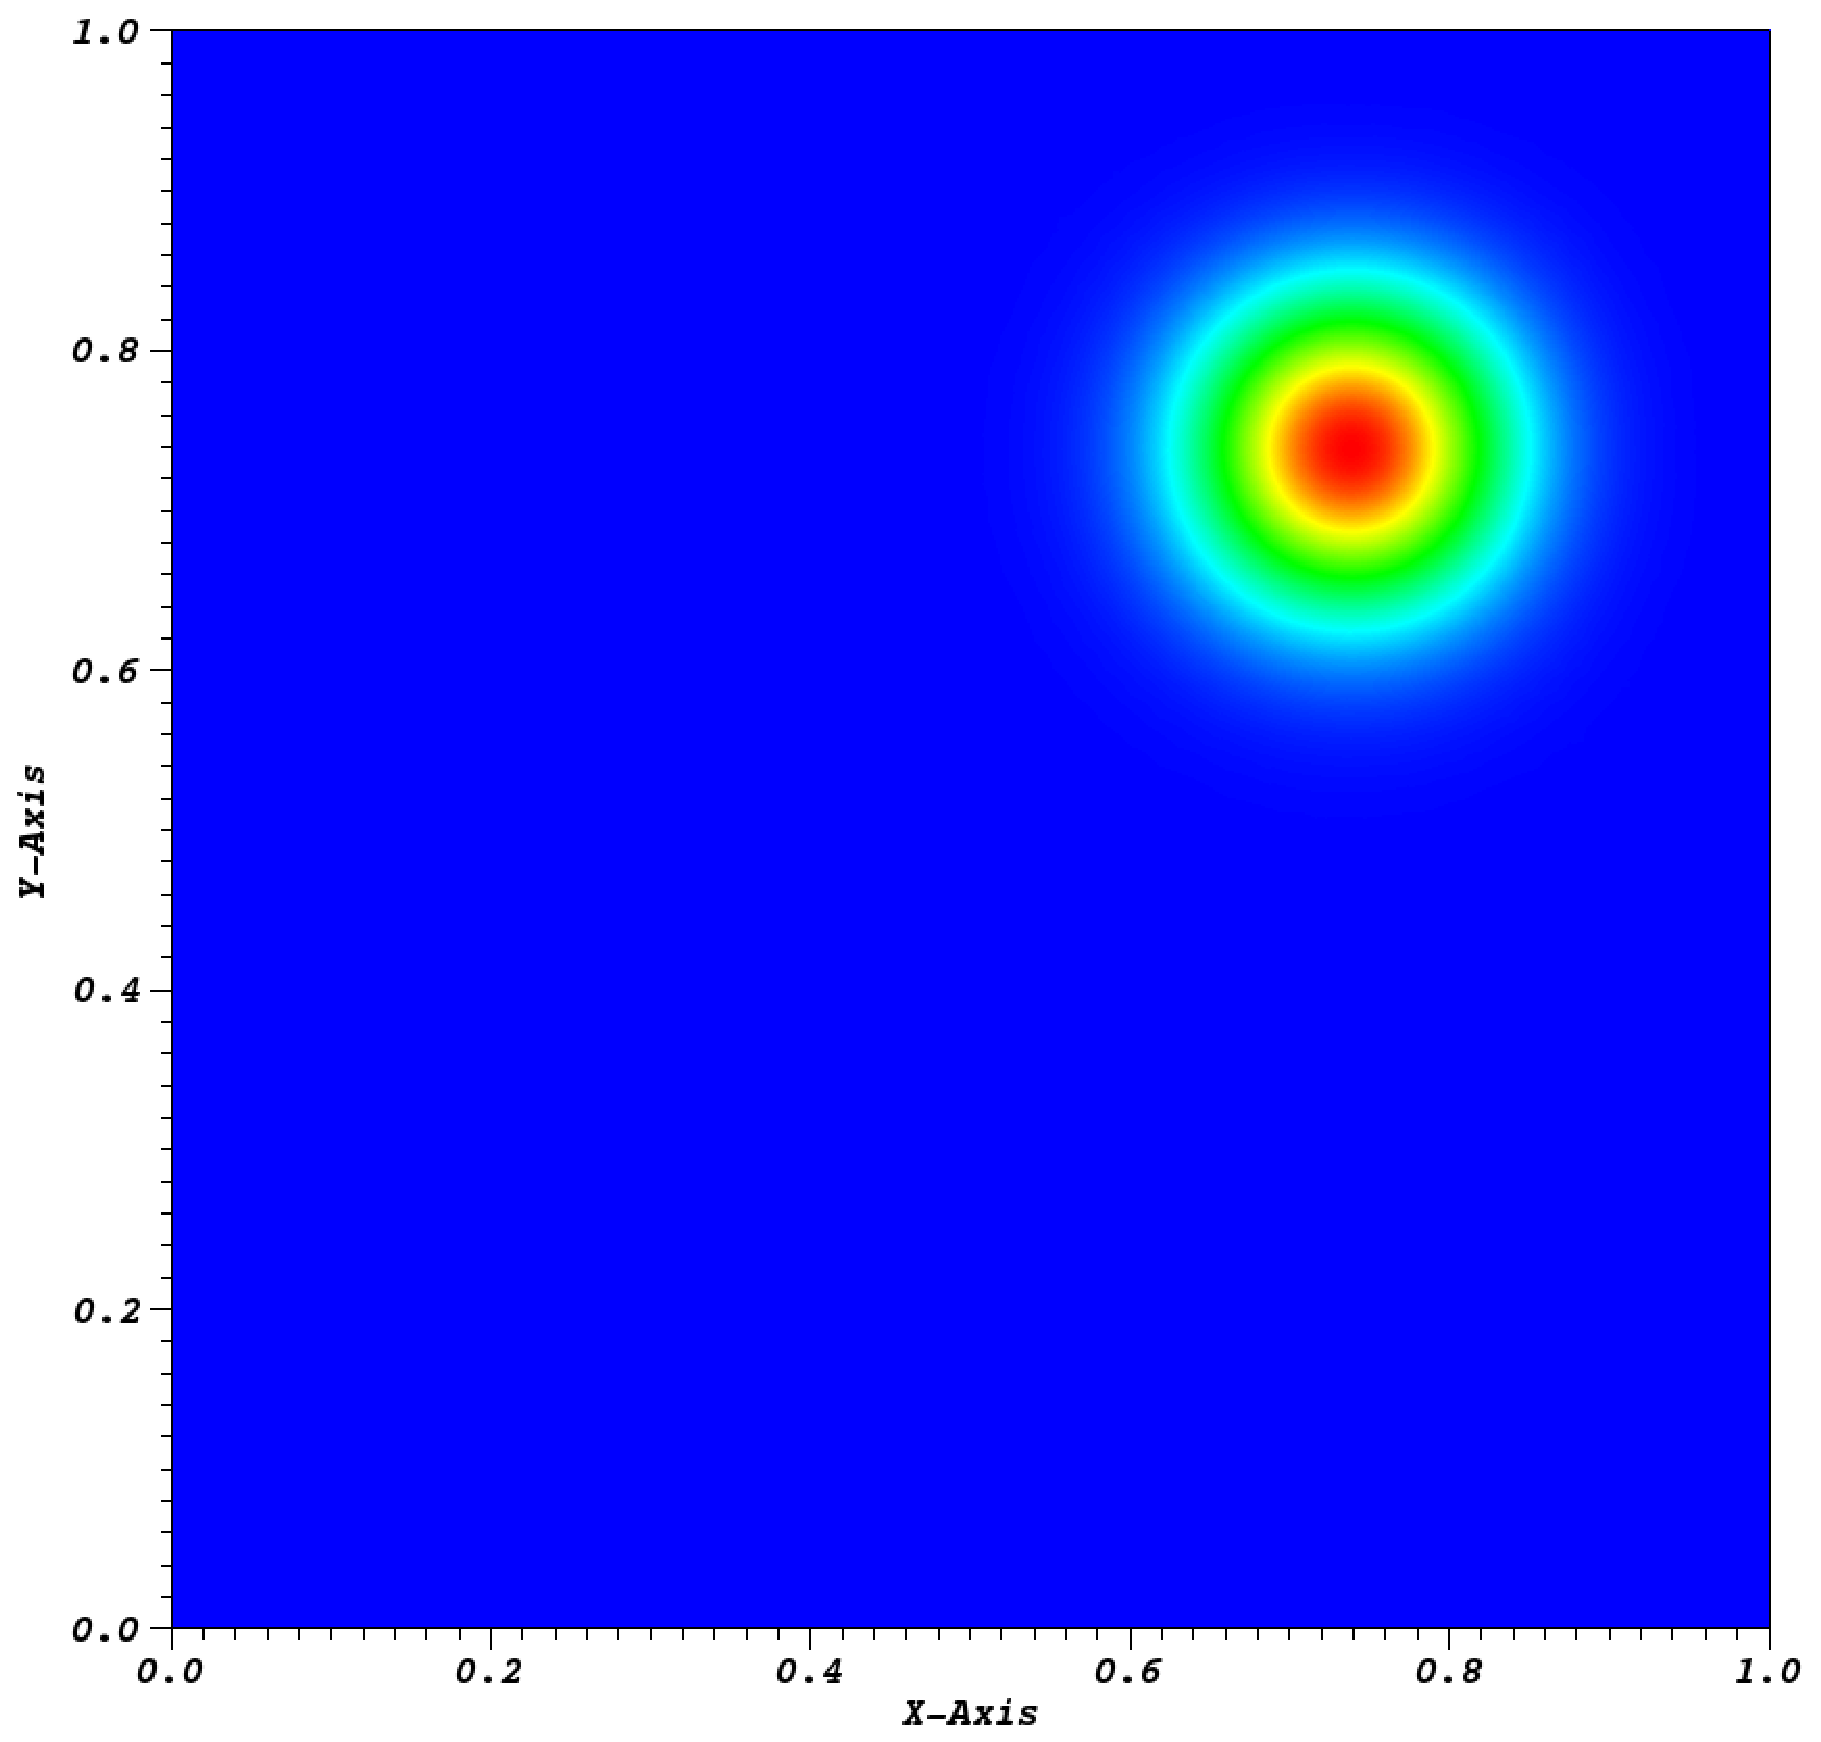
\includegraphics[width=0.70\columnwidth]{images/ME1_cart_Irr=1_tol=0.2_cyc15_sol.eps}
\column{0.50\textwidth}
\centering
{}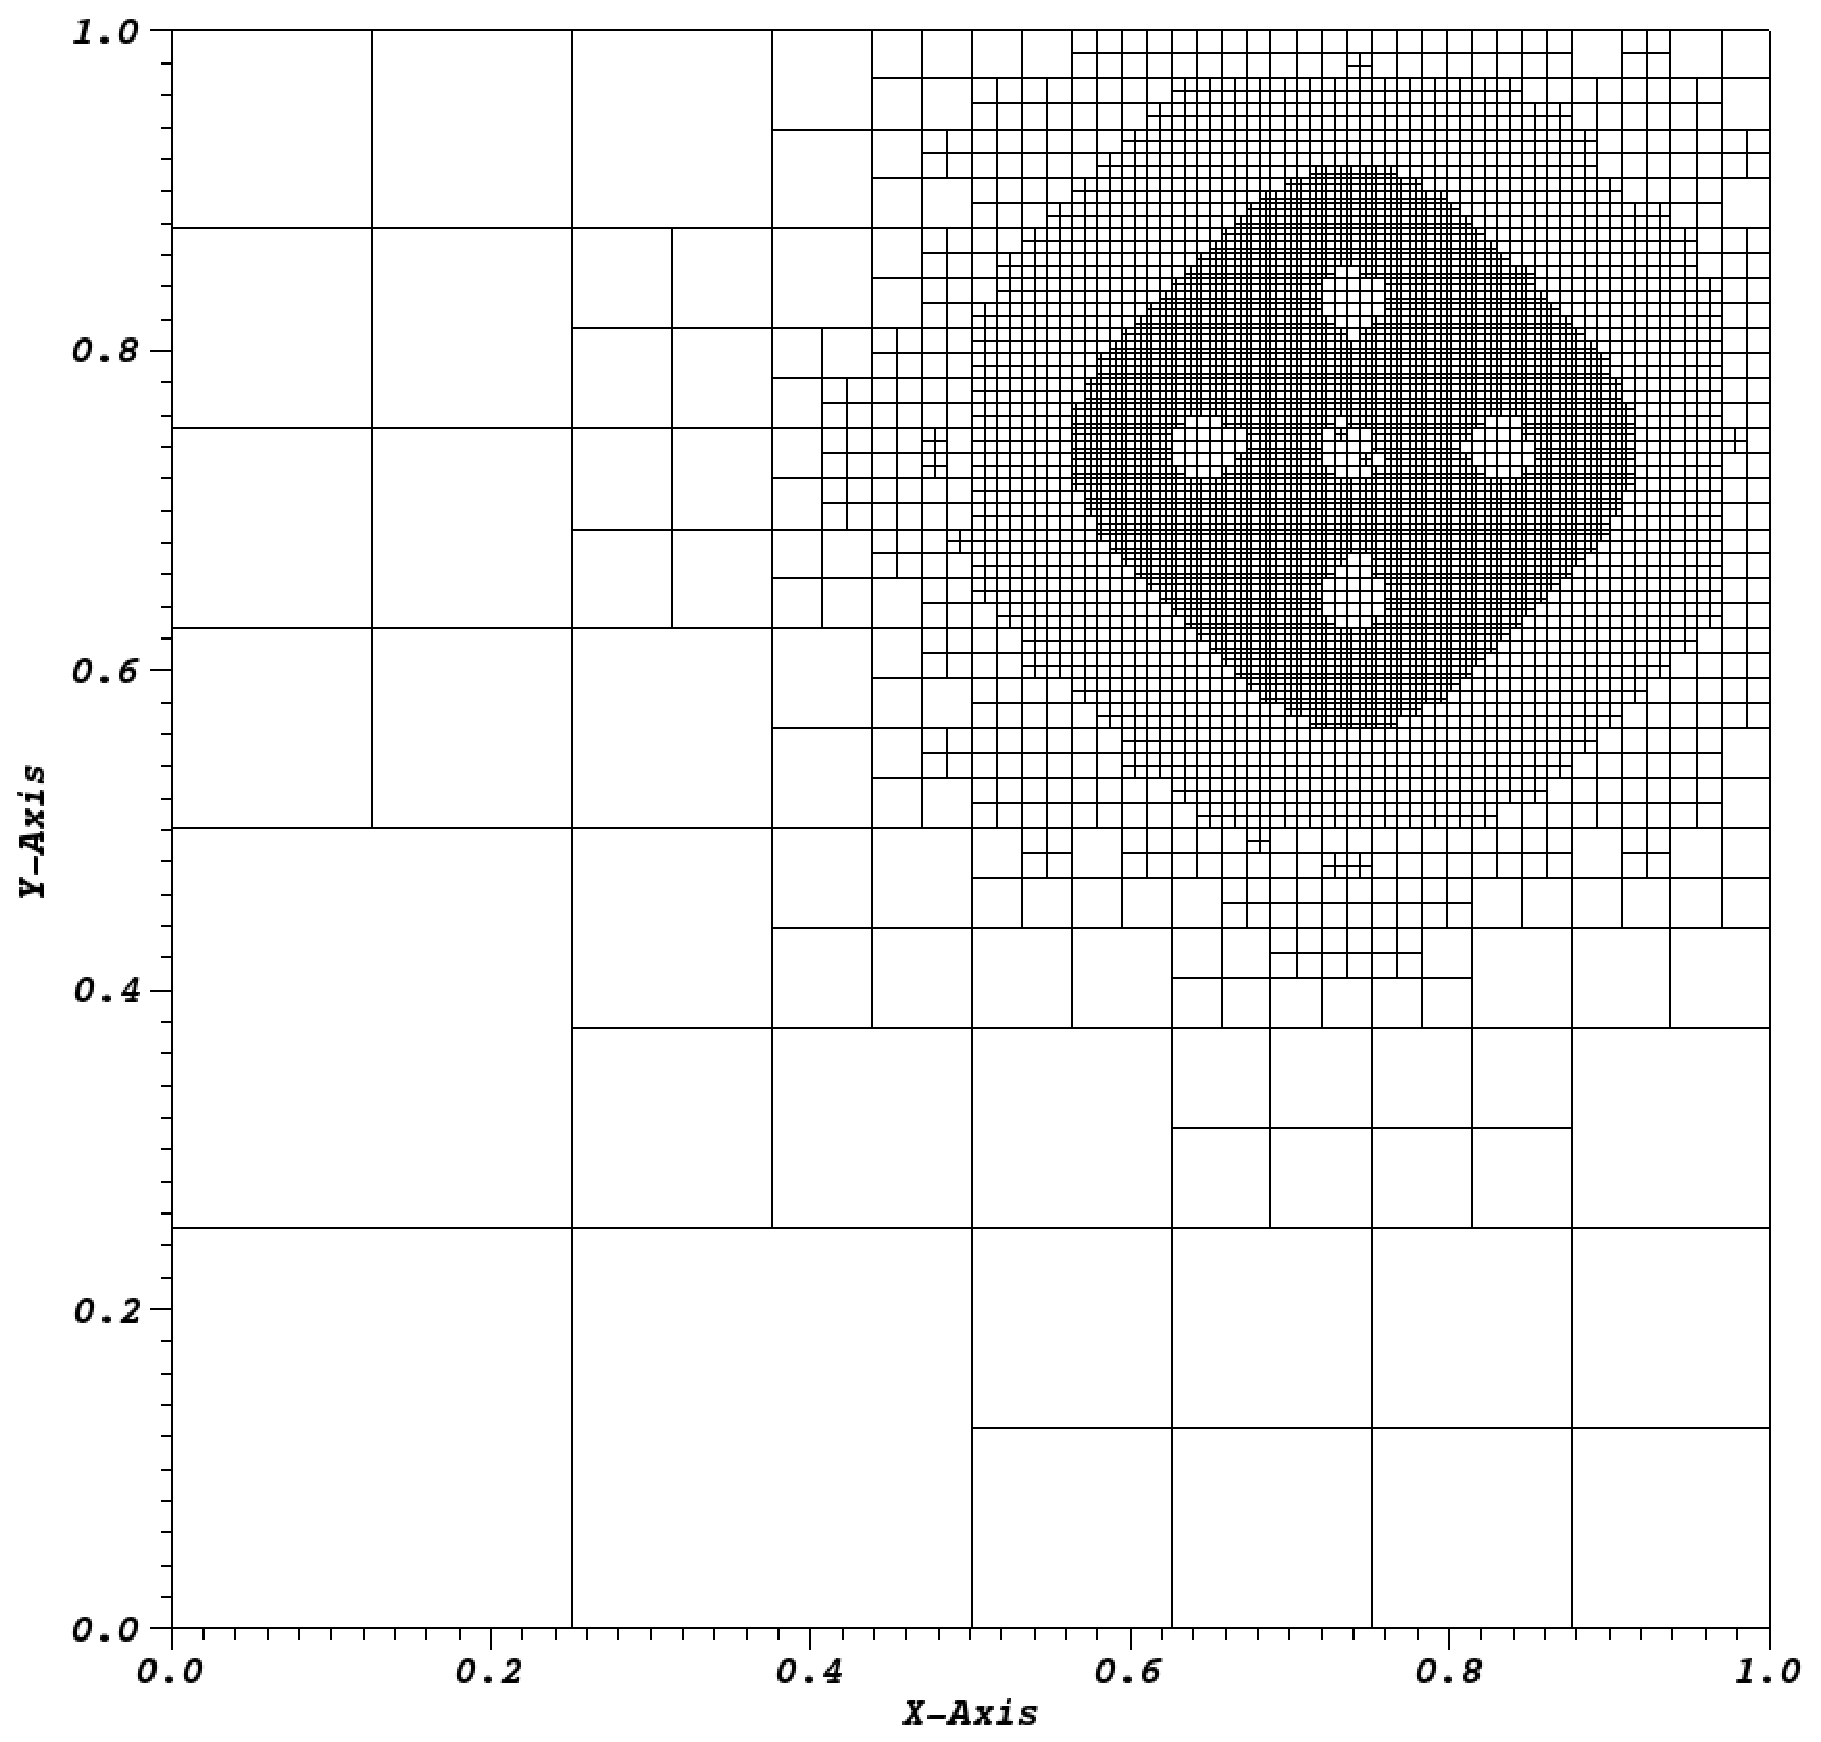
\includegraphics[width=0.70\columnwidth]{images/ME2_cart_Irr=1_tol=0.1_cyc08_mesh.eps} \\
{}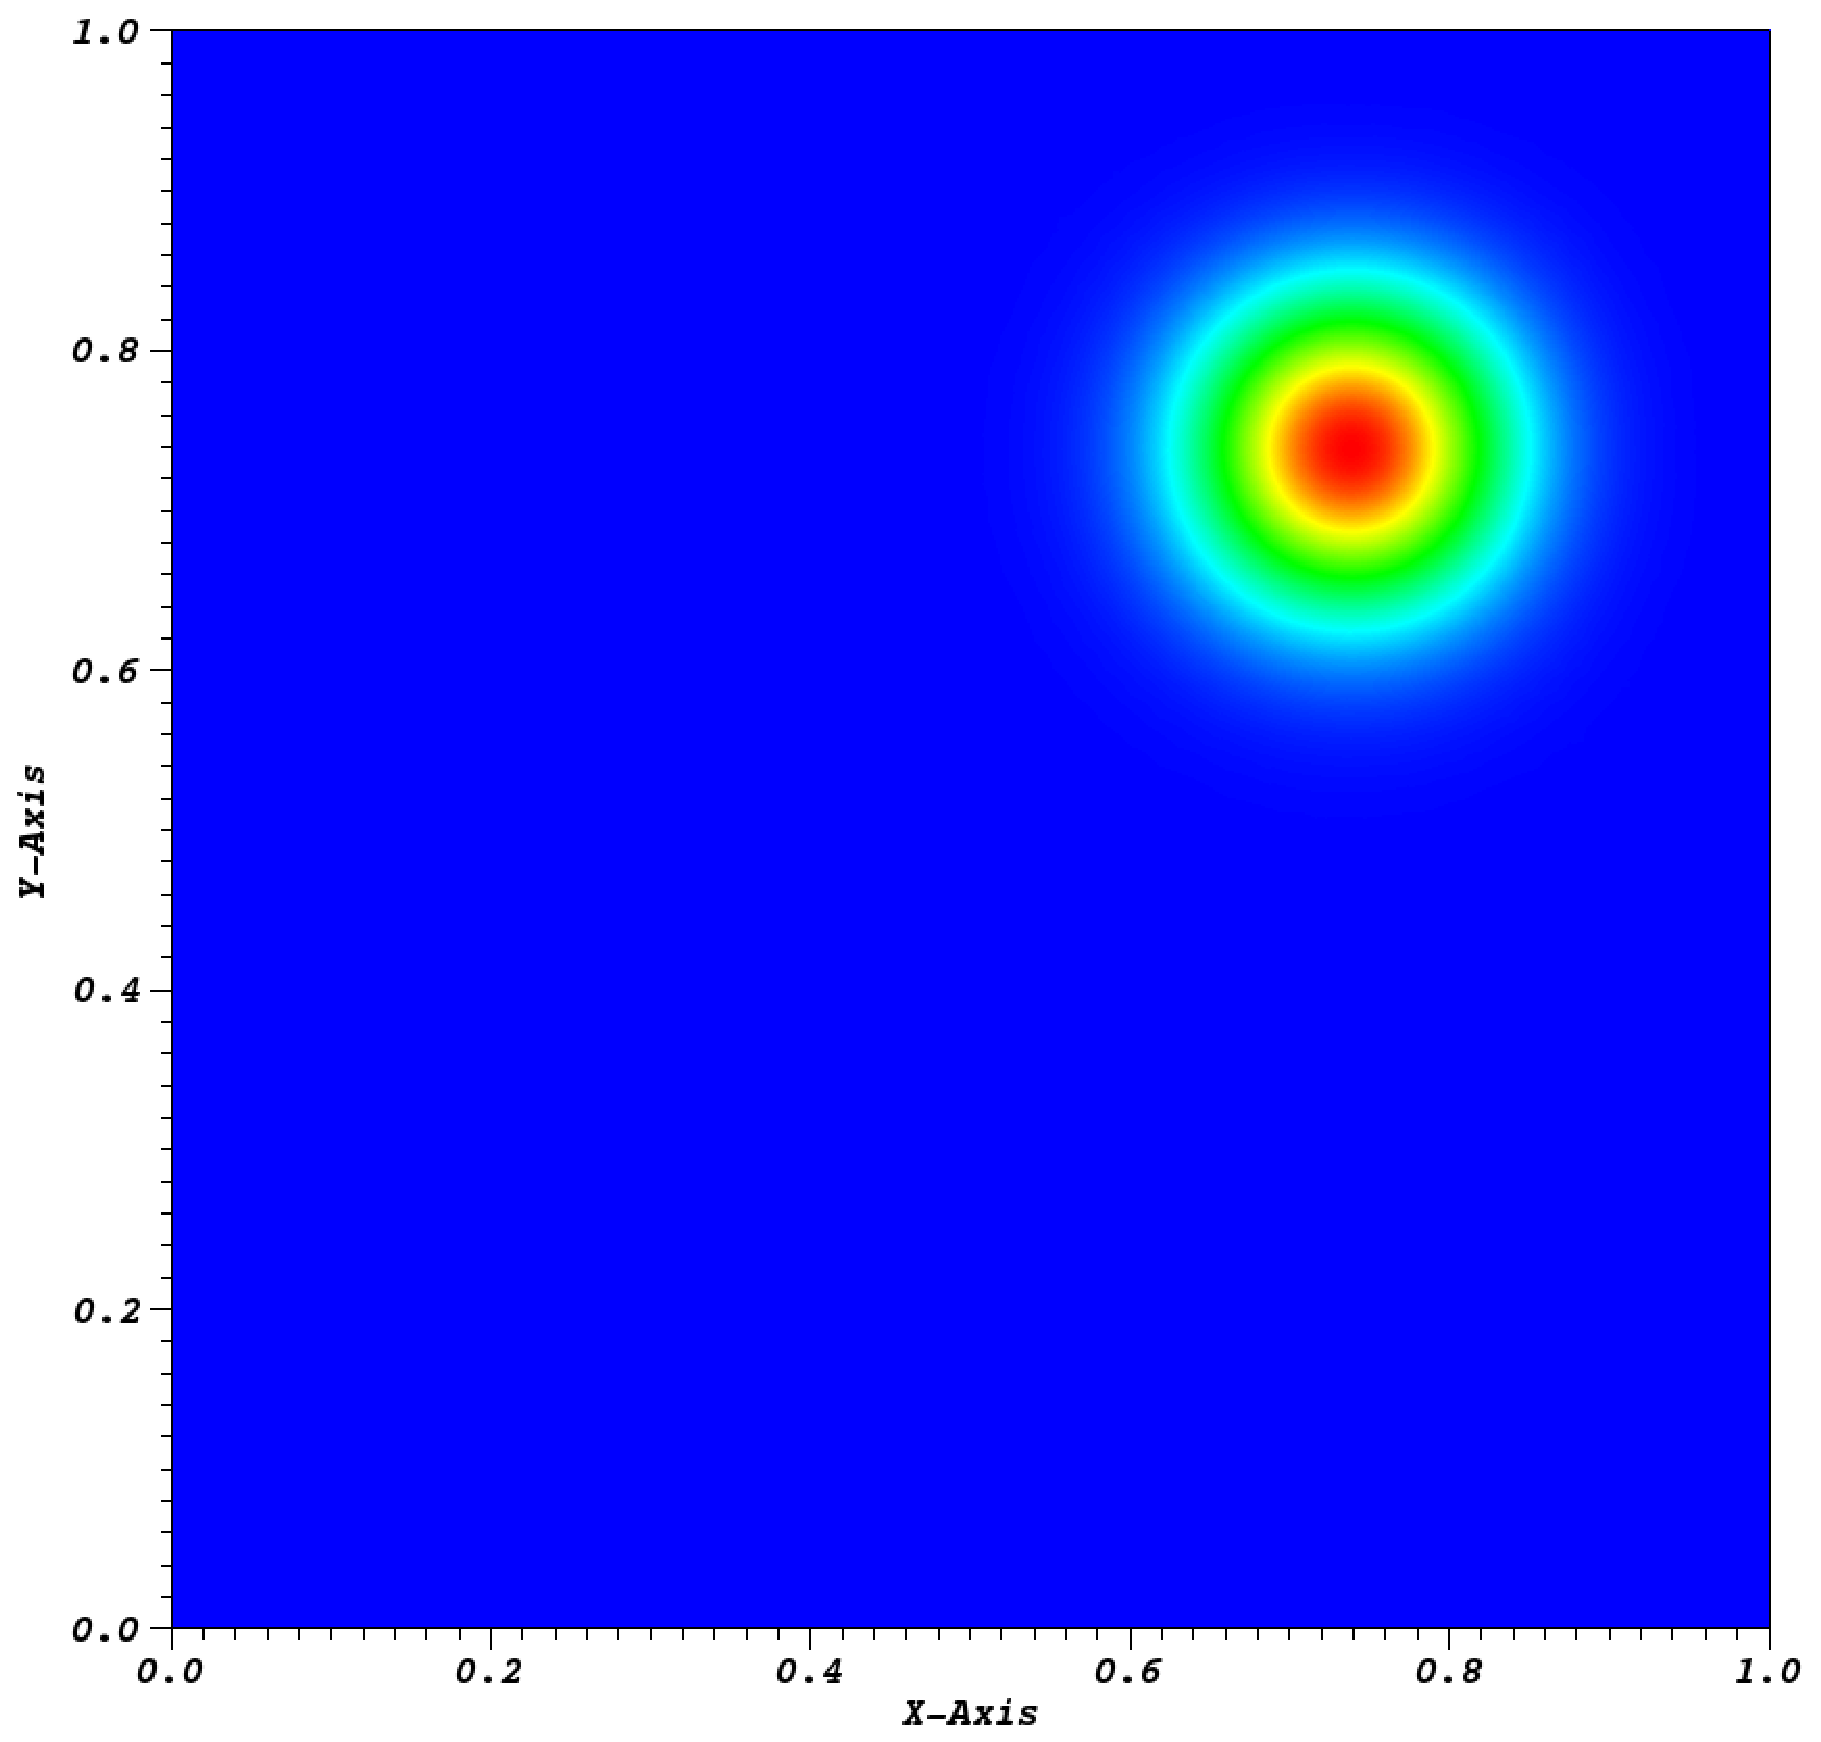
\includegraphics[width=0.70\columnwidth]{images/ME2_cart_Irr=1_tol=0.1_cyc08_sol.eps}
\end{columns}
\end{frame}
%---------------------------
\subsection{}
%---------------------------
\begin{frame}[t]\frametitle{3D FEM/DSA Analysis}
\centering
\vspace{0.2cm}
\includegraphics[width=0.32\textwidth]{images/3D_cart_mesh.eps} 
\includegraphics[width=0.32\textwidth]{images/3D_tri_mesh.eps}
\includegraphics[width=0.32\textwidth]{images/3D_rand_poly_mesh.eps}  \\
\vspace{0.2cm}
\includegraphics[width=0.32\textwidth]{images/3D_shes_poly_mesh.eps} 
\includegraphics[width=0.32\textwidth]{images/3D_sine_poly_mesh.eps} 
\includegraphics[width=0.32\textwidth]{images/3D_z_poly_mesh.eps} 
\end{frame}
%---------------------------
\setbeamerfont{frametitle}{size=\small}
\begin{frame}[t]\frametitle{SIP exactly linear solutions on 3D polyhedral meshes using the PWL basis functions}
\centering
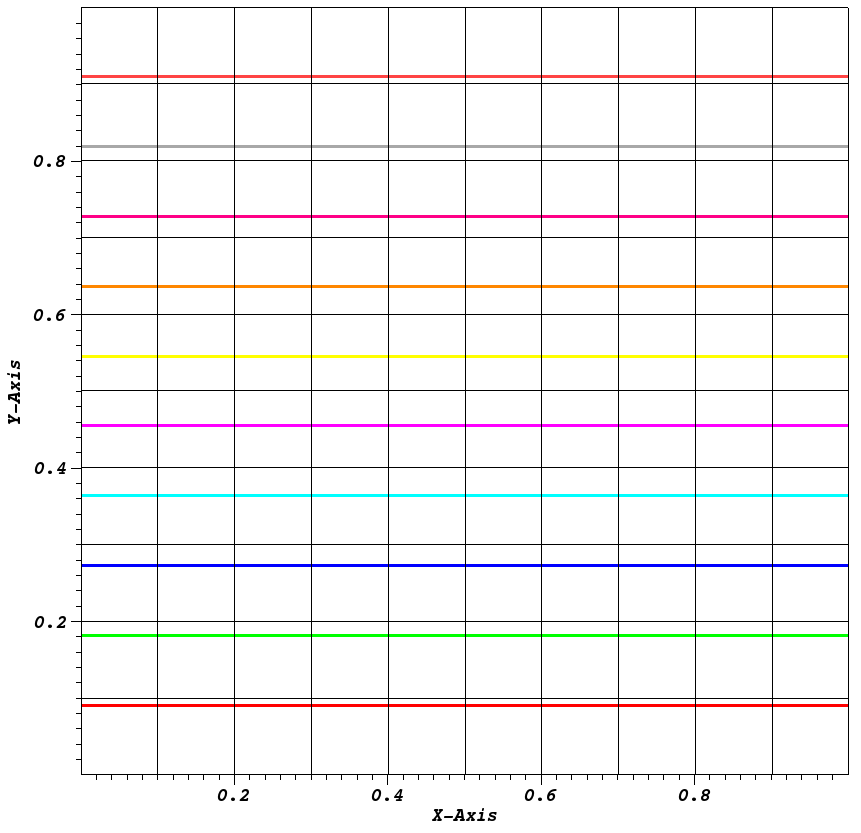
\includegraphics[width=0.32\textwidth]{images/cart_lin_contour.png} 
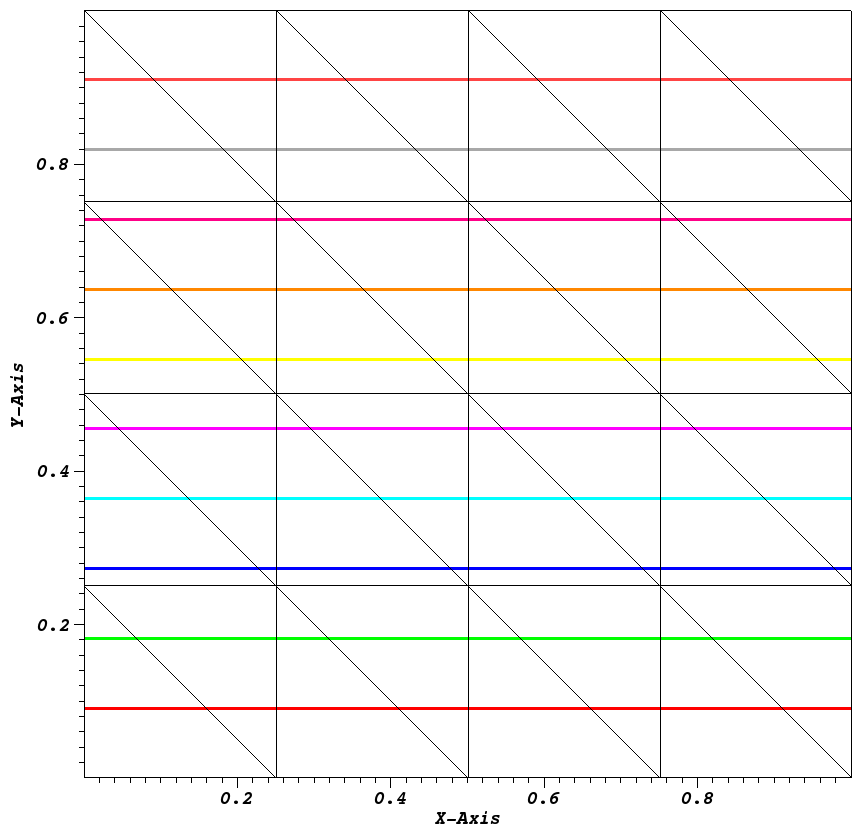
\includegraphics[width=0.32\textwidth]{images/tri_lin_contour.png} \\
\vspace{0.2cm}
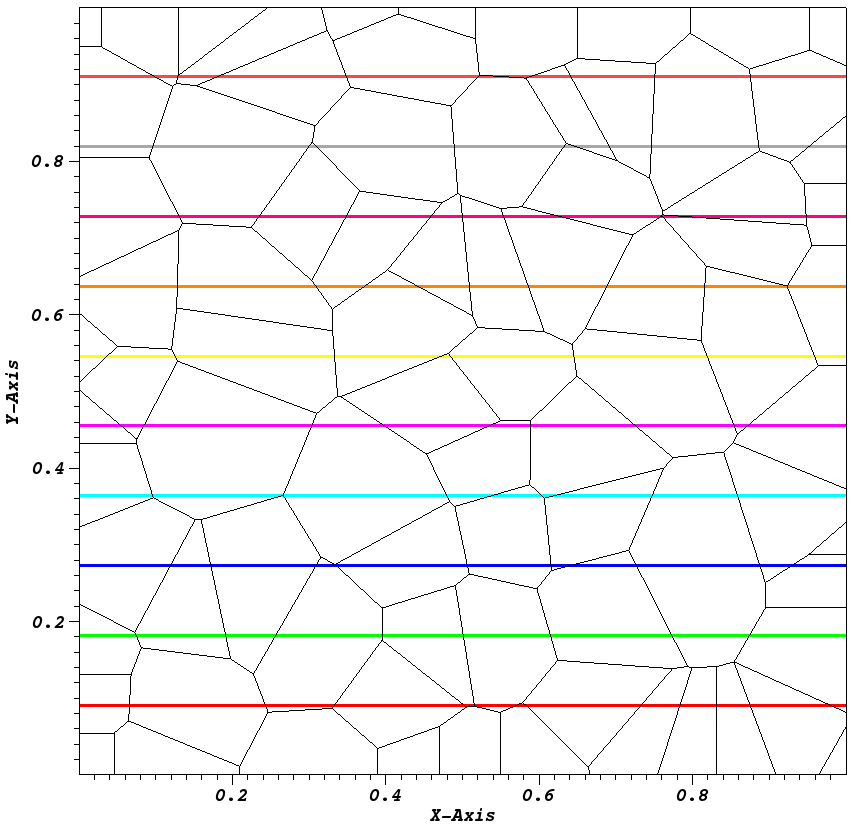
\includegraphics[width=0.32\textwidth]{images/poly_lin_contour.png} 
\includegraphics[width=0.32\textwidth]{images/sine_poly_lin_contour.png} 
\includegraphics[width=0.32\textwidth]{images/z_poly_lin_contour.png} 
\end{frame}
%---------------------------
% QUAD MMS SOLUTION - CURRENTLY COMMENTED OUT
\iffalse
\setbeamerfont{frametitle}{size=\small}
\begin{frame}[t]\frametitle{SIP convergence study - quadratic solution on 3D cube using the PWL basis functions}
\begin{block}{}
	\begin{equation*}
		\begin{aligned}
		\Phi(x,y,z) =& x y z (L_x - x)  (L_y - y)  (L_z - z) \\
		L_x& = L_x = L_x = 1.0
		\end{aligned}
	\end{equation*}
\end{block}
\centering
\includegraphics[width=0.9\textwidth]{images/sip_quad_full_paint.png} 
\end{frame}
\fi
%---------------------------
\setbeamerfont{frametitle}{size=\small}
\begin{frame}[t]\frametitle{SIP convergence study - gaussian solution on 3D cube using the PWL basis functions}
\begin{block}{}
	\begin{equation*}
		\begin{aligned}
		\Phi(x,y,z) = x y z (L_x - x)  (L_y - y)  (L_z - z) \exp(-({\bf r} - {\bf r}_0) \cdot ({\bf r} - {\bf r}_0))\\
		L_x = L_x = L_x = 1.0 , \qquad {\bf r}_0 = (3/4,3/4,3/4)
		\end{aligned}
	\end{equation*}
\end{block}
\centering
\includegraphics[width=0.9\textwidth]{images/sip_gauss_full_paint.png} 
\end{frame}
%---------------------------
\begin{frame}[t]\frametitle{Fourier analysis - 3D PWL basis functions}
\begin{columns}
\column{0.48\textwidth}
\begin{block}{$c=1$}
\centering
{}\includegraphics[width=0.8\textwidth]{images/SI_MIP_hex_C=1_LS2,4,8_F&NSR_PDT.png} \\
{}\includegraphics[width=0.8\textwidth]{images/SI_MIP_hex_LS8_C=1_AR.eps}
\end{block}
\column{0.48\textwidth}
\begin{block}{$c=4$}
\centering
{}\includegraphics[width=0.8\textwidth]{images/SI_MIP_hex_C=4_LS2,4,8_F&NSR_PDT.png} \\
{}\includegraphics[width=0.8\textwidth]{images/SI_MIP_hex_LS8_C=4_AR.eps}
\end{block}
\end{columns}
\end{frame}
%---------------------------
\begin{frame}[t]\frametitle{MIP DSA Timing Data with PDT on Vulcan using HYPRE}
\begin{figure}[t]
\centering
{}\includegraphics[width=0.75\textwidth]{images/Vulcan_DSA_Timing.eps}
\begin{block}{Problem Description}
	\begin{itemize}
	\item Modified Zerr problem - used optimal sweep aggregation parameters
	\begin{itemize}
	\item homogeneous cube - about 500 mfp and c=0.9999
	\item $S8$ level-symmetric quadrature
	\end{itemize}
	\item pointwise convergence tolerance of 1e-8
	\item SI precondition with MIP DSA using HYPRE PCG and AMG
	\end{itemize}
\end{block}
\end{figure}
\end{frame}
%---------------------------
\begin{frame}[t]\frametitle{Two-grid acceleration implementation in PDT}
\begin{block}{}
\begin{itemize}
	\item Successfully implemented and debugged
	\begin{itemize}
		\item Includes non-orthogonal  mesh configurations
		\item Includes multi-material configurations
	\end{itemize}
	\item Have tested the two-grid methodology on a homogeneous graphite block as well as a block with an air duct
	\item Iteration counts for a very large configuration (very optically thick) are similar to simple infinite medium calculations
\end{itemize}
\end{block}
\centering
\vspace{1cm}
\begin{table}
\footnotesize
\begin{tabular}{|c|c|c|}
\hline
Materials & Unaccelerated Iterations & Accelerated Iterations  \\
\hline \hline
Graphite Only & 2027 & 21 \\ \hline
Graphite + Air Duct & 2138 & 23 \\ \hline
\end{tabular}
\end{table}
\end{frame}
%---------------------------
%%%%%%%%%%%%%%%%%%%%%%%%%%%%%%%%%%%%%%%%%%%%%%%%%%%%%%%%%%%%%%%%%%%%%%%%%%%%%%%%%%%%%%%%%%%%%
\typeout{***********************************************************************************}
\typeout{Work Summary}

\section{Work Summary}
\subsection{}
%---------------------------

\begin{frame}[t]\frametitle{Work Summary and Status - completed (blue), in-progress (orange), and not-started (red)}\vspace{-0.2cm}
\begin{block}{POLYFEM}{\footnotesize
\begin{enumerate}
	\item {\color{blue} Analyze the 2D linear polygonal basis functions for use in DGFEM transport calculations}
	\item {\color{blue} Perform the same analysis with the quadratic serendipity basis functions}
	\item {\color{amber} Determine the effects of numerical integration on highly-distorted polygonal elements}
	\item {\color{amber} Perform analysis on benchmark cases using polygonal meshes (including AMR)}
\end{enumerate}}
\end{block}
\begin{block}{MIP DSA}{\footnotesize
\begin{enumerate}
	\item {\color{blue} Analyze the 2D polygonal basis functions with MIP DSA preconditioning through Fourier/numerical analysis}
	\item {\color{blue} Extend the analysis of MIP DSA to arbitrary convex 3D polyhedra}
	\item {\color{amber} Analyze the effects of AMR with polygonal basis functions on the MIP DSA PCG iteration counts (with and without bootstrapping)}
	\item {\color{blue} Implement MIP DSA in PDT using HYPRE}
	\begin{enumerate}{\footnotesize
		\item {\color{blue} Analyze the scalability of the method to high process counts}
		\item {\color{blue} Implement and perform analysis of two-grid acceleration}
		\item {\color{blue} Perform parametric studies on aggregation/partitioning factors} - {\color{amber} generate a performance model of MIP DSA with HYPRE}
		\item {\color{red} Run realistic numerical experiments - IM1 and reactor geometries}
	}\end{enumerate}
\end{enumerate}}
\end{block}
\end{frame}
%---------------------------
%%%%%%%%%%%%%%%%%%%%%%%%%%%%%%%%%%%%%%%%%%%%%%%%%%%%%%%%%%%%%%%%%%%%%%%%%%%%%%%%%%%%%%%%%%%%%
\typeout{***********************************************************************************}
\typeout{We have reached the end}

\begin{frame}[plain]
   \frametitle{I look forward to your feedback regarding my PhD Proposal}

\vspace{25mm}

\begin{columns}[b]

\column{0.7\textwidth}

\centering

{\Large Questions?}

\vspace{9mm}
\footnotesize
A special acknowledgment to the Department of Energy Rickover Fellowship Program in Nuclear Engineering, which provides strong support to its fellows and their professional development.

\end{columns}

\vspace{10mm}

\begin{columns}[b]

\column{0.5\textwidth}
\centering
{}\includegraphics[width=0.35\figwidth]{images/DOE_logo.png}\\

\column{0.5\textwidth}
\centering
{}\includegraphics[width=0.70\figwidth]{images/tamu_engineering.png}\\

\end{columns}

\end{frame}

%%%%%%%%%%%%%%%%%%%%%%%%%%%%%%%%%%%%%%%%%%%%%%%%%%%%%%%%%%%%%%%%%%%%%%%%%%%%%%%%%%%%%%%%%%%

\backupbegin
\appendix

%%%%%%%%%%%%%%%%%%%%%%%%%%%%%%%%%%%%%%%%%%%%%%%%%%%%%%%%%%%%%%%%%%%%%%%%%%%%%%%%%%%%%%%%%%%%
%%%%%%%%%%%%%%%%%%%%%%%%%%%%%%%%%%%%%%%%%%%%%%%%%%%%%%%%%%%%%%%%%%%%%%%%%%%%%%%%%%%%%%%%%%%%
\typeout{***********************************************************************************}
\typeout{Backup Slides}
\section{Backup Slides}
\iffalse
\subsection{Stretch Goals}
%---------------------------
\setbeamerfont{frametitle}{size=\large}
\begin{frame}[t]\frametitle{Stretch Goals}

\end{frame}
%---------------------------
\fi
%%%%%%%%%%%%%%%%%%%%%%%%%%%%%%%%%%%%%%%%%%%%%%%%%%
\subsection{Limits of the 2D linear polygonal FEM basis functions}
%---------------------------
\setbeamerfont{frametitle}{size=\large}
\begin{frame}[t,label=poly_limits]\frametitle{\small Linear POLYFEM limits - Wachspress, mean value, and max entropy (\hyperlink{2D_poly<1>}{\beamergotobutton{Go back}})}
\begin{block}{General form}
\begin{equation*}
\lambda_i (\vec{x}) = \frac{w_i (\vec{x})}{\sum\displaylimits_j w_j (\vec{x})}
\end{equation*}
\end{block}
\begin{columns}
\column{0.45\textwidth}
\begin{block}{\small Nodal limits - $\lim\displaylimits_{\vec{x} \rightarrow \vec{x}_j} \lambda_i (\vec{x}) $}
\begin{equation*}
\begin{aligned}
\lambda_i (\vec{x}) &= \frac{w_i / w_j}{1+ \sum\displaylimits_{k \neq j} w_k / w_j}, \qquad i \neq j \\
\lambda_j (\vec{x}) &= \frac{1}{1+ \sum\displaylimits_{k \neq j} w_k / w_j}
\end{aligned}
\end{equation*} \\ \vspace{2mm}
\begin{equation*}
\lim\displaylimits_{\vec{x} \rightarrow \vec{x}_j} \frac{w_k (\vec{x})}{w_j (\vec{x})} = 0, \qquad k \neq j
\end{equation*}\\ \vspace{2mm}
\begin{equation*}
\therefore \lambda_i (\vec{x}_j) = \delta_{ij}
\end{equation*}
\end{block}
\column{0.52\textwidth}
\vspace{-5mm}
\begin{block}{\small Edge limits - $\lim\displaylimits_{\vec{x} \rightarrow \vec{x}^*} \lambda_i (\vec{x})$, $x^* \in  e_j$}{
\begin{equation*}
\begin{aligned}
\lim\displaylimits_{\vec{x} \rightarrow \vec{x}^*} \left|  w_i (\vec{x})  \right| &= \infty , \qquad i = (j,j+1) \\
\lim\displaylimits_{\vec{x} \rightarrow \vec{x}^*} \left|   w_i (\vec{x})  \right| &< \infty, \qquad i \neq (j,j+1)
\end{aligned}
\end{equation*}\\ \vspace{3mm}
\begin{equation*}
\lim\displaylimits_{\vec{x} \rightarrow \vec{x}^*} \lambda_i (\vec{x}) = 
\begin{cases}
\frac{|| \vec{x}_{j+1} - \vec{x}  ||}{|| \vec{x}_{j+1} - \vec{x}_{j}  ||}, & i=j \\ \, \\
\frac{|| \vec{x}_{j} - \vec{x}  ||}{|| \vec{x}_{j+1} - \vec{x}_{j}  ||}, & i=j+1
\end{cases}
\end{equation*}
}\end{block}
\end{columns}
\end{frame}
%---------------------------
\backupend

\end{document}

